\documentclass[12pt,english]{report}
\renewcommand{\familydefault}{\rmdefault}
\usepackage[latin9]{inputenc}
\usepackage[letterpaper]{geometry}
\geometry{verbose,tmargin=1.25in,bmargin=1.25in,lmargin=1.4in,rmargin=1.15in}
\pagestyle{plain}
\usepackage[doublespacing]{setspace}
\usepackage{tocloft}
\usepackage[rm, tiny,center, compact, uppercase]{titlesec}
\usepackage{indentfirst}
\usepackage{epstopdf}
\usepackage{graphicx,float,wrapfig}
\usepackage{etoolbox}
\usepackage{tocvsec2}
\usepackage[titletoc]{appendix}
\usepackage{tamuconfig}

\usepackage{amsmath}
\usepackage{array}
\usepackage{color}
\usepackage{graphicx}
\usepackage{float} % utiliser H pour forcer a mettre l'image ou on veut
\usepackage{lscape} % utilisation du mode paysage
\usepackage{mathbbol} % permet d'avoir le vrai symbol pour les reels grace a mathbb
\usepackage{enumerate}
\usepackage{marvosym}
\usepackage{moreverb} % permet d'utiliser verbatimtab : conservation la tabulation
\usepackage{stmaryrd} % permet d'utiliser \llbrackedt et \rrbracket : double crochet
\usepackage{url}
\usepackage[noabbrev]{cleveref} % permet d'utiliser cref et Cref (e(E)quation(s) (..)
\usepackage{amsthm}
\usepackage{subfig}
\usepackage{mdwlist} % permet de redefinir l'environnement description
\usepackage{xtab}

\usepackage{afterpage}

\newcommand\bn{\boldsymbol{\nabla}}
\newcommand\bo{\boldsymbol{\Omega}}
\newcommand\br{\mathbf{r}}
\newcommand\la{\left\langle}
\newcommand\ra{\right\rangle}
\newcommand\bs{\boldsymbol}
\newcommand\red{\textcolor{red}}
\newcommand\blue{\textcolor{blue}}
\newcommand\mc{\mathcal}
\newcommand\ldb{\{\!\!\{}
\newcommand\rdb{\}\!\!\}}
\newcommand\llb{\llbracket}
\newcommand\rrb{\rrbracket}

\renewcommand{\(}{\left(}
\renewcommand{\)}{\right)}
\renewcommand{\[}{\left[}
\renewcommand{\]}{\right]}

% Si la description est trop longue elle est coupee en plusieurs ligne
\newenvironment{long_description}%
{
  \begin{basedescript}{
      \desclabelstyle{\nextlinelabel}
      \renewcommand{\makelabel}[1]{%
        \parbox[b]{\textwidth}{\bfseries##1}%
      }%
  \desclabelwidth{2em}}}
  {
  \end{basedescript}
}

\newtheorem{algorithm}{Algorithm}[section]
\newtheorem{criterion}{Criterion}[section]
\newtheorem{definition}{Definition}[section]

%\includeonly{dsa}
\begin{document}
\renewcommand{\tamumanuscripttitle}{Acceleration Techniques for
Discrete-Ordinates Transport Methods with Highly Forward-Peaked Scattering}
\renewcommand{\tamupapertype}{Dissertation}
\renewcommand{\tamufullname}{First Middle Lastname}
\renewcommand{\tamudegree}{Doctor of Philosophy}
\renewcommand{\tamuchairone}{Chair Name}
\newcommand{\tamuchairtwo}{Additional Chair Name}
\renewcommand{\tamumemberone}{Committee Member1}
\newcommand{\tamumembertwo}{Committee Member2}
\newcommand{\tamumemberthree}{Committee Member3}
\renewcommand{\tamudepthead}{Department Head}
\renewcommand{\tamugradmonth}{December}
\renewcommand{\tamugradyear}{2012}
\renewcommand{\tamudepartment}{Department Name}

%%%%%%%%%%%%%%%%%%%%%%%%%%%%%%%%%%%%%%%%%%%%%%%%%%%
%
%  New template code for TAMU Theses and Dissertations starting Fall 2012.  
%  For more info about this template or the 
%  TAMU LaTeX User's Group, see http://www.howdy.me/.
%
%  Author: Wendy Lynn Turner 
%	 Version .9.2
%  Last updated 6/21/2012
%
%%%%%%%%%%%%%%%%%%%%%%%%%%%%%%%%%%%%%%%%%%%%%%%%%%%

%%%%%%%%%%%%%%%%%%%%%%%%%%%%%% 
%% TITLE PAGE
%% The values get updated automatically.  Please do not make changes to this file other than adding/deleting committee members where necessary.
%%%%%%%%%%%%%%%%%%%%%%%%%%%%%%

\providecommand{\tabularnewline}{\\}

%\makeatother

%\usepackage{babel}
%\begin{document}
\begin{titlepage}
\begin{center}
\MakeUppercase{\tamumanuscripttitle}
\vspace{4em}

A \tamupapertype

by

\MakeUppercase{\tamufullname}

\vspace{4em}

\begin{singlespace}

Submitted to the Office of Graduate Studies of \\
Texas A\&M University \\

in partial fulfillment of the requirements for the degree of \\
\end{singlespace}

\MakeUppercase{\tamudegree}
\par\end{center}
\vspace{2em}
\begin{singlespace}
\begin{tabular}{ll}
Approved by: & \tabularnewline
& \cr
% If you have Co-Chairs comment out the 'Chair of Committee' line below and uncomment the 'Co-Chairs of Committee' line.
Chair of Committee, & \tamuchairone\tabularnewline
%Co-Chairs of Committee, & \tamuchairone\tabularnewline & \tamuchairtwo\tabularnewline
Committee Members, & \tamumemberone\tabularnewline
 & \tamumembertwo\tabularnewline
 & \tamumemberthree\tabularnewline
Department Head, & \tamudepthead\tabularnewline

\end{tabular}
\end{singlespace}
\vspace{4em}

\begin{center}
\tamugradmonth \hspace{2pt} \tamugradyear

\vspace{3em}

Major Subject: \tamudepartment \par
\vspace{3em}
Copyright \tamugradyear
\par\end{center}
\end{titlepage}
\pagebreak{}




 % This is simply a file that formats and adds your titlepage, please do not edit this unless you have a specific need. .
\chapter*{ABSTRACT}
\addcontentsline{tic}{part}{ABSTRACT}
\pagestyle{plain}
\pagenumbering{roman}
\setcounter{page}{2}
\indent In this dissertation, advanced numerical methods for highly forward
peaked scattering deterministic calculations are devised, implemented, and
assessed. Since electrons interact with the surrounding environment through
Coulomb interactions, the scattering kernel is highly forward-peaked. 
This bears the consequence that, with standard preconditioning, the standard Legendre
expansion of the scattering kernel requires too many terms for the discretized
equation to be solved efficiently using a deterministic method. The Diffusion
Synthetic Acceleration (DSA), usually used to speed up the calculation when
the scattering is weakly anisotropic, is inefficient for electron transport.
This led Morel and Manteuffel to develop an one-dimensional angular multigrid
(ANMG) which has proved to be very effective when the scattering is highly
anisotropic. Later, Pautz et al. generalized this scheme to multidimensional
geometries, but this method had to be stabilized by a diffusive filter that
degrades the overall convergence of the iterative scheme. In this dissertation, we
recast the multidimensional angular multigrid method without the filter as a
preconditioner for a Krylov solver. This new method is stable independently of
the anisotropy of the scattering and is increasingly more effective and
efficient as the anisotropy increases compared to DSA preconditioning wrapped
inside a Krylov solver. At the coarsest level of ANMG, a DSA step is needed. In
this research, we use the Modified Interior Penalty (MIP) DSA. This DSA was
shown to be always stable on triangular cells with isotropic scattering. 
Because this DSA discretization leads to symmetric definite-positive matrices, 
it is usually solved using a conjugate gradient preconditioned (CG) by SSOR but
here, we show that algebraic multigrid methods are vastly superior than more common
CG preconditioners such as SSOR.

Another important part of this dissertation is dedicated to transport 
equation and diffusion solves on arbitrary polygonal meshes. The advantages of
polygonal cells are that the number of unknowns needed to mesh a domain can be
decreased and that adaptive mesh refinement implementation is simplified:
rather than handling hanging nodes, the adapted computational mesh includes 
different types of polygons. Numerical examples are presented for arbitrary
quadrilateral and polygonal grids.
\pagebreak{}

\chapter*{DEDICATION}
\addcontentsline{toc}{part}{DEDICATION}

\indent aaa

\pagebreak{}

%%%%%%%%%%%%%%%%%%%%%%%%%%%%%%%%%%%%%%%%%%%%%%%%%%%
%
%  New template code for TAMU Theses and Dissertations starting Fall 2012.  
%  For more info about this template or the 
%  TAMU LaTeX User's Group, see http://www.howdy.me/.
%
%  Author: Wendy Lynn Turner 
%	 Version 1.0 
%  Last updated 8/5/2012
%
%%%%%%%%%%%%%%%%%%%%%%%%%%%%%%%%%%%%%%%%%%%%%%%%%%%


%%%%%%%%%%%%%%%%%%%%%%%%%%%%%%%%%%%%%%%%%%%%%%%%%%%%%%%%%%%%%%%%%%%%%%
%%                           ACKNOWLEDGEMENTS
%%%%%%%%%%%%%%%%%%%%%%%%%%%%%%%%%%%%%%%%%%%%%%%%%%%%%%%%%%%%%%%%%%%%%
\chapter*{ACKNOWLEDGEMENTS}
\addcontentsline{toc}{chapter}{ACKNOWLEDGEMENTS}  % Needs to be set to part, so the TOC doesnt add 'CHAPTER ' prefix in the TOC.


\indent Lorem ipsum dolor sit amet, consectetur adipiscing elit. Integer lectus quam, condimentum quis bibendum eu, sollicitudin eget lacus. Praesent non sodales odio. Class aptent taciti sociosqu ad litora torquent per conubia nostra, per inceptos himenaeos. Nulla ac luctus sapien. Morbi cursus sapien eget lorem fermentum hendrerit. Nam ac erat dui, in cursus velit. Vivamus hendrerit porttitor nisi, ut porttitor lorem volutpat eget. In ligula ligula, euismod ut condimentum sit amet, pulvinar sit amet diam. Pellentesque interdum, ipsum ullamcorper consequat dignissim, sem arcu egestas mauris, vitae interdum sem tortor ut ante. Nunc blandit laoreet nisi, non rutrum lorem hendrerit quis. Cras nunc diam, convallis et feugiat at, auctor id libero. Nunc facilisis massa eu eros imperdiet vestibulum. Vestibulum ante ipsum primis in faucibus orci luctus et ultrices posuere cubilia Curae; Donec non velit vitae tortor blandit semper.

Etiam vitae dolor nulla. Ut eros odio, rhoncus eget placerat vitae, elementum ac ante. Proin vitae odio eu nisl pharetra mattis. Pellentesque habitant morbi tristique senectus et netus et malesuada fames ac turpis egestas. Phasellus fermentum lacus consectetur neque consequat ullamcorper. Cras blandit urna non dui consequat molestie. Curabitur viverra nibh at nisi semper faucibus. Nam egestas mauris a enim dignissim nec consectetur tortor rutrum. Mauris at nisi in est luctus congue ut mattis est. Ut pretium, mi quis elementum cursus, ante eros suscipit ligula, ut porttitor elit leo sed turpis. Nam sed dui ligula.


\pagebreak{}
\chapter*{NOMENCLATURE}
\addcontentsline{toc}{part}{NOMENCLATURE}

\begin{xtabular}{ll}
      AGMG & AGgregation-based algebraic MultiGrid \tabularnewline
       AMG & Algebraic MultiGrid method \tabularnewline
       AMR & Adaptive Mesh Refinement method \tabularnewline
      ANMG & ANgular multigrid method \tabularnewline
  ANMG-DSA & ANMG using DSA at the coarsest level \tabularnewline
 ANMG-$P1$ & ANMG using $P1$SA at the coarsest level \tabularnewline
         B & Boltzmann \tabularnewline
       BFP & Boltzmann-Fokker-Planck \tabularnewline
       BLD & BiLinear Discontinuous finite elements \tabularnewline
         c & scattering ratio \tabularnewline
        CG & Conjugate Gradient method \tabularnewline
  $\bs{D}$ & directions-to-moments \tabularnewline
       DSA & Diffusion Synthetic Acceleration \tabularnewline
        FP & Fokker-Planck \tabularnewline
       GLC & Gauss-Legendre-Chebyshev \tabularnewline
     GMRES & Generalized Minimal RESidual method \tabularnewline
  $\bs{L}$ & streaming matrix \tabularnewline
  $\bs{M}$ & moments-to-directions matrix \tabularnewline
       MIP & Modified Interior Penalty \tabularnewline
       MIS & Maximally Independent Sets \tabularnewline
        ML & MultiLevel package of Trilinos \tabularnewline
        MM & Morel and Manteuffel angular multigrid method \tabularnewline
    $P1$SA & $P1$ Synthetic Acceleration \tabularnewline
     $P_l$ & Legendre polynomial of degree $l$ \tabularnewline
   $P_l^m$ & Associated Legendre polynomial of degree $l$ and order $m$
  \tabularnewline
       PAM & Pautz, Adams, and Morel angular multigrid method \tabularnewline
     PAMNF & PAM with No Filtering \tabularnewline
      PWLD & PieceWise Linear Discontinuous finite elements \tabularnewline
  $\tilde{R}$ & mean square stopping power \tabularnewline
       $S$ & restricted stopping power \tabularnewline
  $\tilde{S}$ & stopping power \tabularnewline
        SI & Source Iteration \tabularnewline
     $S_n$ & Discrete ordinates method of order $n$ \tabularnewline
     $SGS$ & Symmetric Gauss-Seidel \tabularnewline
       SPD & Symmetric Positive-Definite \tabularnewline
      SSOR & Symmetric Successive OverRelaxation method \tabularnewline
       $T$ & half of the restricted momentum transfer \tabularnewline
$\tilde{T}$ & half of the momentum transfer \tabularnewline
   $Y_l^m$ & spherical harmonic of degree $l$ and order $m$ \tabularnewline 
     $\bo$ & $(\mu,\varphi)$ unit vector in the flight direction \tabularnewline
     $\mu$ & $\cos(\theta)$ \tabularnewline
   $\mu_0$ & $\bo'\cdot \bo$ \tabularnewline
    $\psi$ & angular flux \tabularnewline
$\bs{\Sigma}$ & scattering cross sections matrix \tabularnewline
$\Sigma_a(\br,E)$ & absorption macroscopic cross section \tabularnewline
$\Sigma_s(\br,E)$ & scattering macroscopic cross section \tabularnewline
$\Sigma_s(\br,\bo'\cdot\bo,E'\rightarrow E)$ & differential scattering macroscopic 
  cross section \tabularnewline
$\Sigma_t(\br,E)$ & total macroscopic cross section \tabularnewline
  $\theta$ & directional polar angle \tabularnewline
 $\varphi$ & directional azimuthal angle \tabularnewline
\end{xtabular}

\pagebreak{}

%%%%%%%%%%%%%%%%%%%%%%%%%%%%%%%%%%%%%%%%%%%%%%%%%%%
%
%  New template code for TAMU Theses and Dissertations starting Fall 2012.  
%  For more info about this template or the 
%  TAMU LaTeX User's Group, see http://www.howdy.me/.
%
%  Author: Wendy Lynn Turner 
%	 Version 1.0 
%  Last updated 8/5/2012
%
%%%%%%%%%%%%%%%%%%%%%%%%%%%%%%%%%%%%%%%%%%%%%%%%%%%
%%%%%%%%%%%%%%%%%%%%%%%%%%%%%%%%%%%%%%%%%%%%%%%%%%%%%%%%%%%%%%%%%%%%%%
%%       TABLE OF CONTENTS
%%%%%%%%%%%%%%%%%%%%%%%%%%%%%%%%%%%%%%%%%%%%%%%%%%%%%%%%%%%%%%%%%%%%%
\phantomsection
\addcontentsline{toc}{chapter}{TABLE OF CONTENTS}  % Needs to be set to part, so the TOC doesnt add 'CHAPTER ' prefix in the TOC.
\begin{singlespace}
\renewcommand\contentsname{\normalfont} {\centerline{TABLE OF CONTENTS}}

%\setcounter{tocdepth}{4} % This puts \subsubsection[]{×} in your List of Tables.  The default is 3.


%%%%%%%%%%%%%  Adds Page above the page number in TOC
\setlength{\cftaftertoctitleskip}{1em}
\renewcommand{\cftaftertoctitle}{%
\hfill{\normalfont {Page}\par}}



\tableofcontents

\end{singlespace}

\pagebreak{}

%%%%%%%%%%%%%%%%%%%%%%%%%%%%%%%%%%%%%%%%%%%%%%%%%%%%%%%%%%%%%%%%%%%%%%
%%                           lIST OF FIGURES
%%%%%%%%%%%%%%%%%%%%%%%%%%%%%%%%%%%%%%%%%%%%%%%%%%%%%%%%%%%%%%%%%%%%%

\phantomsection
\addcontentsline{toc}{chapter}{LIST OF FIGURES}  % Needs to be set to part, so the TOC doesnt add 'CHAPTER ' prefix in the TOC.

\renewcommand{\cftloftitlefont}{\center\normalfont\MakeUppercase}

\setlength{\cftbeforeloftitleskip}{-12pt} %% Positions the LOF title vertically to match the chapter titles

\renewcommand{\cftafterloftitleskip}{12pt}
\renewcommand{\cftafterloftitle}{%
\\[\baselineskip]\mbox{}\hfill{\normalfont Page}}

\begingroup


\begin{center}
\begin{singlespace}
%% These values make the lof table entries appear double spaced between.
\setlength{\cftbeforechapskip}{0.4cm}
\setlength{\cftbeforesecskip}{0.30cm}
\setlength{\cftbeforesubsecskip}{0.30cm}
\setlength{\cftbeforefigskip}{0.4cm}
\setlength{\cftbeforetabskip}{0.4cm}
\listoffigures

\end{singlespace}
\end{center}
\pagebreak{}


%%%%%%%%%%%%%%%%%%%%%%%%%%%%%%%%%%%%%%%%%%%%%%%%%%%%%%%%%%%%%%%%%%%%%%
%%                           lIST OF TABLES
%%%%%%%%%%%%%%%%%%%%%%%%%%%%%%%%%%%%%%%%%%%%%%%%%%%%%%%%%%%%%%%%%%%%%%
%
\phantomsection
\addcontentsline{toc}{chapter}{LIST OF TABLES}  % Needs to be set to part, so the TOC doesnt add 'CHAPTER ' prefix in the TOC.

\renewcommand{\cftlottitlefont}{\center\normalfont\MakeUppercase}

\setlength{\cftbeforelottitleskip}{-12pt} %% Positions the LOF title vertically to match the chapter titles

\renewcommand{\cftafterlottitleskip}{12pt}
\renewcommand{\cftafterlottitle}{%
\\[\baselineskip]\mbox{}\hfill{\normalfont Page}}

\begin{center}
\begin{singlespace}

%% These values make the lot table entries appear double spaced between.
\setlength{\cftbeforechapskip}{0.4cm}
\setlength{\cftbeforesecskip}{0.30cm}
\setlength{\cftbeforesubsecskip}{0.30cm}
\setlength{\cftbeforefigskip}{0.4cm}
\setlength{\cftbeforetabskip}{0.4cm}
\listoftables

\end{singlespace}
\end{center}
\endgroup
\pagebreak{}  % Need this for the pagenumbering to be correct.   % This is simply a file that formats and adds your toc, lof, and lot, please do not edit this unless you have a specific need. .


\chapter{\uppercase{Modified Interior Penalty on Arbitrary Polygonal Cells}}
\label{mip_chapter}
\section{Introduction}
In Chapter \ref{anmg_chapter}, we noted that at the coarsest level of ANMG 
a Diffusion Synthetic Acceleration needs to be solved. 
Because analytical and closed form solutions are unavailable for most
radiation transport problems of practical interest, one typically employs
iterative techniques to solve the large system of equations that results from
the spatial and angular discretization of the transport equation. Standard
iterative techniques for the first-order form of the discrete-ordinate ($S_n$)
transport equation include the Source Iteration (SI) technique and Krylov 
subspace algorithms (usually GMRes). For highly diffusive materials (i.e., 
with scattering ratios $c=\Sigma_s / \Sigma_t $ close to 1) and optically 
thick configurations (i.e., not leakage dominated), these iterative techniques 
can become quite ineffective, requiring high iteration counts and possibly 
leading to false convergence. However, SI and GMRes-based transport solves 
can be accelerated (preconditioned) with DSA approaches 
\cite{dsa_ref,larsen_dsa,consistent_p1,m4s,wla,mip}. 

It is well established that the spatial discretization of the DSA equations
must be somewhat ``consistent'' with the one used for the $S_n$ transport equations to
yield unconditionally stable and efficient DSA schemes
(\cite{dsa_ref,larsen_dsa,consistent_p1,m4s,wla,mip}). However, 
consistency between the discretized transport equations and the discretized
diffusion may not be computationally practical (especially for unstructured
arbitrary meshes, \cite{dsa_ref}). For instance, Warsa, Wareing, and
Morel \cite{consistent_p1} derived a fully consistent DSA scheme for linear
discontinuous finite elements on unstructured tetrahedral meshes; their DSA
scheme yielded in a $P_1$ system of equations which was found to be
computationally more expensive than partially consistent DSA schemes that are
based upon discretizations of a standard diffusion equation. Some partially 
consistent schemes have been analyzed for linear discontinuous finite element
(DFE) discretizations of the transport equation on unstructured meshes, for
instance, the modified-four-step (M4S) scheme \cite{m4s}, the
Wareing-Larsen-Adams (WLA) scheme \cite{wla,wla_pwl}, and the Modified Interior
Penalty (MIP) scheme \cite{mip}.

We will come back to DSA later but first, we want to point the usefulness of
using polygonal or polyhedral cells. Such cell types may present some advantages over
traditional cells types (simplices, hexahedra) and have found some
applications in radiation transport \cite{pwld_2d,pwld_3d,cfm_dfm}. 
Some general motivations for
polyhedral cells are as follows. Simplicial cell types (triangles, tetrahedra)
can produce good  quality mesh for highly complex geometries, but are not
well suited to capture boundary layers and are prone to numerical diffusion.
Quadrilaterals and hexahedra have been shown to be less numerically diffusive
than simplicial meshes \cite{??}, but may be harder to employ for complicated
geometries. Polyhedral cells retain the attractive features of hexahedral
cells  (the number of polyhedra is often much smaller than that of tetrahedral
cells for an equivalent accuracy), while allowing for meshing
flexibility (boundary layer meshes can easily be set up, polyhedral meshes can
be generated from tetrahedral meshes, polyhedra can be included locally in
existing meshes to improve mesh quality). Meshing tools such as MSTK
\cite{mstk} and the Computational Geometry Algorithms Library \cite{cgal} may
be employed to process polyhedral meshes. For example, the radiation transport
code PDT and the CFD codes Fluent and OpenFOAM offer polyhedral mesh and
solver capabilities.

The following features of polygonal and polyhedral cells are noteworthy:
\begin{itemize}
 \item \underline{Reduced number of unknowns per cell.} To illustrate this, we
   assume one unknown per vertex in every cell, which is standard for
   transport discretizations that perform well in the thick diffusive regime.
   In the 2D hexagonal example of Figure \ref{fig_hexa_split}, the number of
   unknowns would be six (one unknown per vertex). Using triangular cells, the
   same hexagon would have to be split into four triangles at least (thus 12
   unknowns) or possibly six triangles to preserve symmetry (thus 18 unknowns in
   that case). Similarly, using quadrilateral cells, the hexagon would be
   bisected into two quadrilaterals at least (8 unknowns), but divisions into
   three or four quadrilaterals are also possible (thus, 12 or 16 unknowns).
   \begin{figure}[H]
   \centering
   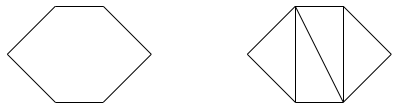
\includegraphics[width=0.5\textwidth]{./Dsa/hex_tri_cells}
   \caption{Hexagonal cell versus triangle cells.}
   \label{fig_hexa_split}
   \end{figure}
 \item \underline{Transition elements and Adaptive Mesh Refinement.} Solvers
   based on arbitrary polyhedral cells can easily handle cells with various
   numbers of edges (2D) and faces (3D). This can be particularly useful for
   simulations with Adaptive Mesh Refinement (AMR)
   \cite{amr_rad,amr_block,amr_unstruc}, without having to deal with the
   implementation of data structures to handle hanging nodes
   \cite{arbitrary_hanging_nodes,dealII_hanging_nodes,locally_hanging_nodes}.
   On Figure \ref{fig_amr}, the left cell is a pentagon whereas the two cells 
   on the right
   are quadrilaterals (a similar illustration can be made for 3D hexahedral
   AMR meshes: suppose a cell is connect to four cells through one of its faces
   - a standard situation with AMR on hexahedral grids - ; such a cell can be
   thought of as a 9-face polyhedron). Thus, a method based on a piecewise linear
   discretization can handle locally adapted meshes without any special
   treatment or further approximation of the coupling between cells.
   \begin{figure}[H]
   \centering
   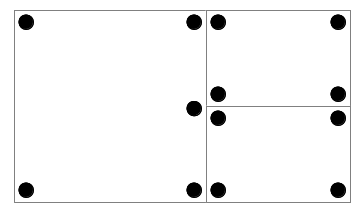
\includegraphics[width=0.3\textwidth]{./Dsa/amr}
   \caption{AMR mesh.}
   \label{fig_amr}
   \end{figure}
\end{itemize}
Several discretization methods haven been developed for 
arbitrary polygonal meshes \cite{pwld_2d,pwld_3d,cfm_dfm,pwl_diffusion,
palmer_fe,mimetic,cell_centered_diff,palmer_proc,palmer_ane,wachspress,pwbld}.
In this work, we focus on the PWLD discretization \cite{pwld_2d,pwld_3d}. This
discretization can be applied for any polygonal cells and the integrals
generated by this discretization can be easily computed analytically. 

As of today, a lot of the ongoing effort to develop a DSA scheme on
polygonal/polyhedral cells focuses on adapting the WLA scheme on polygonal meshes
\cite{cfm_dfm,wla_pwl}. The WLA scheme is a two-stage process, where first a
diffusion solution is obtained using a {\em continuous} finite element
discretization and then a {\em discontinuous } update is performed cell-by-cell 
in order to provide an appropriate discontinuous scalar flux to the DFE transport 
solver. In \cite{consistent_p1}, the WLA scheme was
found to be a stable and effective DSA technique, though its efficiency
degraded as the problem became more optically thick and highly diffusive.
To the authors' best knowledge, no work is currently done to adapt the M4S 
technique to polygonal/polyhedral meshes. This is probably due to the fact
that, even though the scheme is effective in one-dimensional slab and
two-dimensional rectangular geometries, it was found to be divergent as an
accelerator for SI in
three-dimensional tetrahedral meshes with linear discontinuous elements.
Furthermore, the scheme does not yield a Symmetric Positive Definite (SPD)
matrix. In this paper, we present an extension of the MIP technique to the
PWLD discretization techniques for for arbitrary polygonal/polyhedral meshes.
The MIP scheme is based on the standard Interior Penalty (IP) for the
discontinuous discretization of diffusion equations. MIP was first derived in
\cite{mip}, where it was applied to triangular unstructured meshes (with
locally adapted cells). MIP did not suffer the degradation of efficiency 
than WLA when the
problem becomes optically thick and highly diffusive and it is therefore an
interesting alternative to WLA. To our knowledge, this work presented the
first DSA scheme based on the same discontinuous trial spaces as the transport
finite element discretization for such meshes. Because MIP produces SPD
equations, it has been solved using conjugate gradient (CG) preconditioned by
a symmetric successive over-relaxation method (SSOR) in \cite{mip}. Here, the
effectiveness of algebraic multigrid methods (AMG) to precondition diffusion
solver \cite{amg,amg_course} will be tested and comparer with CG+SSOR.
Algebraic multigrid methods allow the use of multigrid techniques when no grid
information is available or when the grid is unstructured. Instead of using a
succession of grids based on the geometry of the problems, the ``grid levels''
are based on properties of the matrix.

\addtocontents{toc}{\protect\afterpage{\hfill{Page}\par\medskip}}
\addtocontents{toc}{\protect\afterpage{\vspace{-10pt}\hfill{}\par\medskip}}
\addtocontents{lof}{\protect\afterpage{\hspace{-33pt}{FIGURE}\hfill{Page}\par\medskip}}
\addtocontents{lof}{\protect\afterpage{\vspace{-10pt}\hfill{}\par\medskip}}
\addtocontents{lot}{\protect\afterpage{\hspace{-31pt}{TABLE}\hfill{Page}\par\medskip}}
\addtocontents{lot}{\protect\afterpage{\vspace{-10pt}\hfill{}\par\medskip}}

\section{Transport equation}
Inelastic interactions, collisional and radiative scattering, can be divided
into two classes : ``catastrophic" interactions that result in large-energy
losses and ``soft" interactions that result in small-energy losses. p25 CEPXS


\chapter{\uppercase{Spatial discretizations}} \label{spatial_chapter}
\section{Introduction}
In this Chapter, we introduce the two spatial discretizations used
in this research: the BiLinear Discontinuous finite elements (BLD) 
\cite{thick_dgfem,lumping_bld} and the PieceWise Linear Discontinuous finite 
elements (PWLD) \cite{pwld_3d,pwld_2d}. The BLD discretization is being used on
rectangular cells whereas PWLD is being used on arbitrary convex polygonal
cells. Both of these discretizations give the correct result in the diffusion 
limit. Using finite elements to spatially discretize \cref{transport_sn}, we
get after expanding $\psi_s$ and $\phi$ on the basis functions $b_j^K(\br)$, 
multiplying the equation by the test function $b_i^K(\br)$, and integrating 
on the cell $K$ (the superscript $K$ is used for a variable defined on $K$):
\begin{equation}
  \begin{split}
    &\int_{K} b_i^K(\br) \bo_d \cdot \bn \(\sum_j \psi_{d,j}^K b_j^K(\br)\)\ d\br + 
    \int_{K} b_i^K(\br) \Sigma_t^K(\br) \(\sum_j \psi_{d,j}^K b_j^K(\br)\)\ d\br =\\
    &\int_{K} b_i^K(\br) \sum_{l=0}^L \Sigma_{s,l}^K(\br) \sum_{m=-l}^l
    \(\sum_j \phi_{l,m,j}^K b_j^K(\br)\) Y_l^m(\bo_d)\ d\br + \int_{K} b_i^K(\br)
    Q_d^K(\br)\ d\br
  \end{split}
\end{equation}
where $\oint_{\partial K}$ is the integral over the boundary $\partial K$ of
cell $K$ and $\bs{n}_b^K$ is the external normal. Using Stokes' theorem, the 
previous equation becomes:
\begin{equation}
  \begin{split}
    &\oint_{\partial K} b_i^K(\br) \bo_d \cdot \bs{n}_b^K \(\sum_j \psi_{d,j}^K
    b_j^K(\br)\)\ d\br -\int_{K} \(\sum_j \psi_{d,j}^K b_j^K(\br)\) \bo_d \cdot 
    \bn b_i^K(\br)\ d\br +\\
    &\int_{K} b_i^K(\br) \Sigma_t^K(\br) \(\sum_j \psi_{d,j}^K b_j^K(\br)\)\ d\br =
    \int_{K} b_i^K(\br) \sum_{l=0}^L \Sigma_{s,l}^K(\br) \times\\
    &\sum_{m=-l}^l \(\sum_j \phi_{l,m,j}^K b_j^K(\br)\) Y_l^m(\bo_d)\ d\br + 
    \int_{K} b_i^K(\br) Q_d^K(\br)\ d\br
  \end{split}
\end{equation} 
Using upwind on the first term of the previous equation, we obtain:
\begin{equation}
  \begin{split}
    &\oint_{\partial K} b_i^K(\br) \bo_d \cdot \bs{n}_b^K \(\sum_j \psi_{d,j}^K 
    b_j^K(\br)\)\ d\br = \int_{\partial J \cap \partial K} b_i^{J}(\br) \bo_d 
    \cdot \bs{n}_b^J  \times\\
    &\(\sum_j \psi_{d,j}^J b_j^J(\br)\)d\br+ \int_{\partial K\backslash\(
    \partial J \cap \partial K\)} b_i^K(\br) \bo_d \cdot \bs{n}_b^K \(\sum_j 
    \psi_{d,j}^K b_j^K(\br)\)d\br
  \end{split}
\end{equation}
where $J$ is a cell adjacent to $K$ associated to the edge of $K$ such that
$\bs{n}_B^K \cdot \bo_d < 0$, $\partial J$ is the boundary of $J$, and
the basis functions $b_j^J$ and test function $b_i^J$ are defined on $J$.\\
Because of the upwinding, the $S_n$ equation can be solved by sweeping over
the mesh along each direction. During a sweep, the cells are ordered in a list
such that the discretized transport equation can be solved by inversing a
block lower triangular matrix. Sweeping is possible only if all the cells are
convex. Thus, for a direction $d$ and a test function $b_i^K(\br)$ defined on
$K$, we get the equation:
\begin{equation}
  \begin{split}
    &\int_{\partial J \cap \partial K} b_i^{J}(\br) \bo_d \cdot \bs{n}_b^J  \times
    \(\sum_j \psi_{d,j}^J b_j^J(\br)\)d\br+ \int_{\partial K\backslash\(
    \partial J \cap \partial K\)} b_i^K(\br) \bo_d \cdot \bs{n}_b^K \times\\
    &\(\sum_j\psi_{d,j}^K b_j^K(\br)\)d\br - \int_{K} \(\sum_j \psi_{d,j}^K 
    b_j^K(\br)\) \bo_d \cdot \bn b_i^K(\br)\ d\br +\\
    &\int_{K} b_i^K(\br) \Sigma_t^K(\br) \(\sum_j \psi_{d,j}^K b_j^K(\br)\)\ d\br =
    \int_{K} b_i^K(\br) \sum_{l=0}^L \Sigma_{s,l}^K(\br) \times\\
    &\sum_{m=-l}^l \(\sum_j \phi_{l,m,j}^K b_j^K(\br)\) Y_l^m(\bo_d)\ d\br + 
    \int_{K} b_i^K(\br) Q_d^K(\br)\ d\br
  \end{split}
  \label{spatial_sn}
\end{equation}
Assuming that $Q$ and $\Sigma$ are constant by cell, the following
integrals can be precomputed and used in \cref{spatial_sn}:
\begin{align}
  & \int_{\partial J \cap \partial K} b_i^{J}(\br) b_j^J(\br) d\br
  \label{precomputed_1}\\
  & \int_{\partial K\backslash\(\partial J \cap \partial K\)} b_i^K(\br)  
  b_j^K(\br) d\br \label{precomputed_2}\\
  & \int_K b_j^K(\br) \bn b_i^K(\br)\ d\br \label{precomputed_3}\\
  & \int_K b_i^K(\br) b_j^K(\br) d\br \label{precomputed_4}\\
  & \int_K b_i^K(\br)\ d\br \label{precomputed_5}
\end{align}

\section{The $S_n$ Transport Equations}
Given an angular quadrature set $\{\bo_d,w_d\}_{1\leq d \leq M}$, the
one-group $_n$ transport equation with isotropic source and scattering is:
\begin{equation}
  \(\bo_d \cdot \bn +\Sigma_t (\br)\)\psi_d(\br) = \frac{1}{4\pi}\Sigma_s
  (\br)\phi(\br) + \frac{1}{4\pi} S(\br),\ \textrm{ for } \br \in \mc{D},\
  1\leq d \leq M,
  \label{one_speed}
\end{equation}
with $\psi_d(\br)=\psi(\br,\bo_d)$ the angular flux at position $\br$ in
direction $\bo_d$, $\Sigma_t$, and $\Sigma_s$ the total and scattering cross
section, respectively, and $\mc{D}$ the spatial domain. The scalar flux is
defined and evaluated as follows:
\begin{equation}
  \psi(\br) \equiv \int_{4\pi} \psi(\br,\bo)\ d\bo \simeq \sum_{d=1}^M w_d
  \psi_d\(\br\).
  \label{flux_moments}
\end{equation}
The system of equations is closed assuming incoming boundary conditions on
(with $\partial \mc{D} = \partial \mc{D}^{d} \cap \partial \mc{D}^r$):
\begin{equation}
  \psi_d (\br_b) = \left\{
  \begin{aligned}
    &\psi_d^{inc}(\br_b), &\br_b \in \partial \mc{D}^{d,-}=\{\partial \mc{D}^d
    \textrm{ such that } \bo_d \cdot \bs{n}_b <0\} \\
    &\psi_{d^{\prime}}(\br_b), & \br_b \in \partial \mc{D}^{r,-}_d = \{
    \partial \mc{D}^r \textrm{ such that } \bo_d \cdot \bs{n} < 0\}
  \end{aligned}
  \right. ,
\end{equation}
where $\bs{n}_b = \bs{n}(\bs{r}_b)$ is the outward unit normal vector on the
boundary. The reflecting direction of $\bo_d$ at a point $\br_b$ on the
boundary is given by:
\begin{equation}
  \bo_{d^{\prime}} = \bo_d - 2\(\bo_d \cdot \bs{n}_b\)\bs{n}_b.
\end{equation}
We assume the angular quadrature set satisfies the following two conditions
for any outward unit normal vector on the reflecting boundary $\partial
\mc{D}^r$:
\begin{itemize}
  \item $\forall d=1,\hdots,M$, the reflected direction $\bo_{d^{\prime}}$ is
    also in the quadrature set (which is simple to obtain for rectangular
    geometries);
  \item the weights of the incident and reflected directions are equal, i.e.,
    $w_d=w_{d^{\prime}}$
\end{itemize}

For the time being, we assume that no reflective boundaries exist $\(\partial
\mc{D}^r = 0\)$. Then, \cref{one_speed} can be written in a compact form using
operators:
\begin{align}
  &\bs{L}\Psi = \bs{M\Sigma} \Phi + S = q, \label{transport_op}\\
  &\Phi = \bs{D} \Psi, \label{phi_D_psi}
\end{align}
where $\Psi$ is the vector of angular fluxes, $\Phi$ the vector flux moments
(with isotropic scattering, the only moment required is the scalar flux), $q$
is the total (scattering+external) source, $\bs{L}$ is the streaming operator,
$\bs{M}$ is the moment-to-direction operator, and $\bs{D}$ is the
direction-to-moment operator.
$\bs{L}=diag(\bs{L}_1,\hdots,\bs{L}_d,\hdots,\bs{L}_M)$ is a diagonal
operator; given the total source $q$, one can solve independently for the
resulting angular fluxed in all directions. \Cref{transport_op,phi_D_psi} can
be re-arranged in terms of the scalar flux only:
\begin{equation}
  \Phi = \bs{D L}^{-1} \(\bs{M \Sigma}\Phi+S\).
\end{equation}
The action of $\bs{D}\bs{L}^{-1}$ is often referred to as a \emph{transport sweep}
when discontinuous spatial approximations (finite differences, finite
elements) are employed because, for any directions $\bo_d$, the action of
$\bs{L}_d^{-1}$ can be obtained by traversing the mesh (i.e., sweeping) in a
specific ordering of the cells, thus one needs only to solve a small linear
system of equations, cell by cell. The order in which the elements are solved
constitutes the graph of the sweep; above, we have discussed situations where
the graph does not present some dependencies (cycles). Note that cycles in the
sweep graph can also appear due to reflective boundary conditions. These graph
dependencies can either be lagged within the iterative procedure of the
solution vector consisting of the scalar flux is augmented by the angular flux
unknowns that cause the cycles. We will explain these details in the paragraph
related to iterative techniques, but first we generalize our operator
notations for situations where we need to keep in the solution vector both the
flux moments and some angular fluxes dur to dependencies in the graph (non
convex meshed and/or reflective boundaries).

If the graph of the sweep presents dependencies, we practically break the
transport sweep on these boundaries and introduce the notion of significant
angular fluxes. In this situation, we define a matrix $\bs{N}$ that extracts
from the entire angular flux vector all out-going angular fluxes on the
boundaries causing a dependency in the graph of the sweep, i.e., the
significant angular flux vector is given by:
\begin{equation}
  \Psi_{SAF} = \bs{N} \Psi,
\end{equation}
$\bs{N}$ is simply an operator that extracts from the entire angular flux vector,
the values required to break the graph dependencies. We then split the loss
and streaming operator $\bs{L}$ into two parts:
\begin{equation}
  \bs{L} = \underline{\bs{L}} - \overline{\bs{L}},
\end{equation}
where $\underline{\bs{L}}$ is the lower block triangular matrix (which can be
inverted during a transport sweeps) and $\overline{\bs{L}}$ is the strictly
upper triangular block, causing the dependencies in the sweep
($\overline{\bs{L}}$ only contains integrals along some incoming edges of a
cell). Note that $\bs{N}^T\bs{N}$ is a diagonal operator that contains 1 only
for angular flux values that are labeled as ``significant''. Then, we have:
\begin{equation}
  \overline{\bs{L}} \Psi = \overline{\bs{L}} \bs{N}^T\bs{N}\Psi =
  \overline{\bs{L}}\bs{N}^T \Psi_{SAF},
\end{equation}
and can, therefore, re-cast the transport equation as:
\begin{align}
  &\underline{\bs{L}}\Psi =\overline{\bs{L}}\bs{N}^T \Psi_{SAF} + \bs{M\Sigma}
  \Phi + S,\\
  &\Phi = \bs{D}\Psi.
\end{align}

\section{Solution Techniques}
\subsection{Unaccelerated Procedures}
\Cref{transport_op,phi_D_psi} can be solved using the Source Iteration (SI)
method (a stationary iterative technique also known as Richardson iteration).
The SI technique at the $l^{th}$ iteration is given by:
\begin{equation}
  \Phi^{(l+1)} = \bs{DL}^{-1} \(\bs{M \Sigma}\Phi^{(l)} + S\).
\end{equation}
Alternatively, a subspace Krylov method (usually GMRES) can be employed to
solve the following transport system of equations:
\begin{equation}
  \(\bs{I}-\bs{DL}^{-1} \bs{M\Sigma}\)\Phi = \bs{DL}^{-1}S.
\end{equation}
Both the SI and the GMRES approaches require transport sweeps (the action of
$\bs{L}^{-1}$ is required in both procedures).

When the scattering ratio $c=\frac{\Sigma_s}{\Sigma_t}$ tends to one in
optically thick domains, the number of SI and GMRES can become large. Fourier
analyses (for continuous, i.e., undiscretized transport) confirmed that SI
attenuates rapidly error modes associated with high frequencies (transport
dominated modes) while leaving almost unaffected low-frequency error modes
(diffusion dominated modes) \cite{dsa_ref}. To accelerate the convergence, a DSA
preconditioner is thus needed; in addition, some level of consistency is
necessary between the spatial discretization of the transport operator and
than of the diffusion operator. In Chapter \ref{mip_chapter}, we will adapt
the MIP discontinuous finite element discretization of the diffusion equation
for arbitrary polygonal grids is and employ MIP as a DSA preconditioner.

For completeness, we provide the SI and GMRES solution techniques in the case
graph dependencies are present. During one SI iteration, the scalar flux and
the angular significant flux are updated as follows:
\begin{equation}
  \begin{bmatrix}
    \Phi\\
    \Psi_{SAF}
  \end{bmatrix}^{(l+1)}
  = 
  \begin{bmatrix}
    \bs{D}\underline{\bs{L}}^{-1} \bs{M\Sigma} & \bs{D}\underline{\bs{L}}^{-1}
    \overline{\bs{L}}^{-1}\bs{N}^T\\
    \bs{N}\underline{\bs{L}}^{-1} \bs{M\Sigma} & \bs{N}\underline{\bs{L}}^{-1}
    \overline{\bs{L}}^{-1}\bs{N}^T
  \end{bmatrix}
  \begin{bmatrix}
    \Phi\\
    \Psi_{SAF}
  \end{bmatrix}^{(l)}
  +
  \begin{bmatrix}
    \bs{D}\\
    \bs{N}
  \end{bmatrix}
  \underline{\bs{L}}^{-1} S.
  \label{si_matrix_notation}
\end{equation}
\Cref{si_matrix_notation} is simply coded by appending the $\Psi_{SAF}$ to the
scalar flux unknowns (after a transport sweep, the operator $\bs{D}$ is
applied to yield the newest scalar flux whereas the operator $\bs{N}$ is
applied to update the significant angular flux). Note that when
$\overline{\bs{L}}=0$ (i.e., no dependencies in the sweep), we obtain the
standard SI formula:
\begin{equation}
  \Phi^{(l+1)} = \bs{DL}^{-1} \(\bs{M\Sigma}\Phi^{(l)} + S\).
  \label{matrix_form_si}
\end{equation}
From the SI formula of \cref{si_matrix_notation}, it follows that the linear
system for a GMRES-based transport solves is simply:
\begin{equation}
  \(\bs{I}-\bs{T}\)x=b,
\end{equation}
with:
\begin{align}
  &\bs{T} = 
  \begin{bmatrix}
    \bs{D}\underline{\bs{L}}^{-1}\bs{M\Sigma} &
    \bs{D}\underline{\bs{L}}^{-1}\overline{\bs{L}}\bs{N}^T\\
    \bs{N}\underline{\bs{L}}^{-1}\bs{M\Sigma} & \bs{N}
    \underline{\bs{L}}^{-1} \overline{\bs{L}}\bs{N}^T
  \end{bmatrix}                                      
  ,\\
  &x =
  \begin{bmatrix}
    \Phi\\
    \Psi_{SAF}
  \end{bmatrix}
  ,\\
  &b=
  \begin{bmatrix}
    \bs{D}\\
    \bs{N}
  \end{bmatrix}
  \underline{\bs{L}}^{-1}S.
\end{align}

\subsection{Synthetic Acceleration and Preconditioning}
Ignoring graph dependencies for simplicity of the presentation, the transport
equation is:
\begin{equation}
  \(\bs{L}-\bs{M\Sigma D}\)\Psi = S.
  \label{te_1}
\end{equation}
It is often computationally effective write the above linear system as (sweep
preconditioning):
\begin{equation}
  \(\bs{I}-\bs{L}^{-1}\bs{M\Sigma D}\) \Psi = \bs{L}^{-1}S
\end{equation}
because $\bs{L}$ is easier to invert than $(\bs{L}-\bs{M\Sigma D})$. Therefore,
an iterated scheme (the SI technique) yields formally:
\begin{equation}
  \Psi^{(\ell+1)}=\bs{L}^{-1}\(\bs{M\Sigma D}\Psi^{(\ell)}+S\).
\end{equation}
The error equation is:
\begin{equation}
  \begin{split}
    \Psi-\Psi^{(\ell+1)} &= \bs{L}^{-1} \bs{M\Sigma D}\(\Psi - \Psi^{(\ell)}\)\\
                      &= \bs{L}^{-1}\bs{M\Sigma D}\(\Psi-\Psi^{(\ell+1)} +
    \Psi^{(\ell+1)}-\Psi^{(\ell)}\),
  \end{split}
\end{equation}
that is, the transport equation satisfied by the angular error
$\epsilon^{(\ell+1)}=\Psi-\Psi^{(\ell+1)}$ is:
\begin{equation}
  \(\bs{L}-\bs{M\Sigma D}\)\epsilon^{(\ell+1)} = \bs{M\Sigma
  D}\(\Psi^{(\ell+1)}-\Psi^{(\ell)}\).
  \label{ang_err_eq}
\end{equation}
This equation is of the same form as \cref{te_1} (where the source term is now
the scattering due to the difference in successive flux iterates) and,
therefore, is just as difficult to solve. However, solving it would provide
the exact additive term required to obtain the exact solution:
\begin{equation}
  \Psi = \Psi^{(\ell+1)} + \epsilon^{(\ell+1)}
\end{equation}
Since the diffusion error modes are not efficiently attenuated by the above SI
process, it is natural to seek a low-order error equation. Taking the $0^{th}$
and $1^{st}$ angular moment moment of \cref{ang_err_eq}, one obtains a
diffusion equation for the scalar $\varepsilon$:
\begin{equation}
  \bs{A}\epsilon^{(\ell+1)} = \Sigma \(\Phi^{(\ell+1)}-\Phi^{(\ell)}\)
\end{equation}
where $\bs{A}$ is the diffusion operator. However, the scalar correction
$\epsilon^{(\ell+1)}$, when added to the previous iterate of the scalar flux
$\Phi^{(\ell+1)}$, will not yield the exact scalar flux solution because the
low-order error equation is not strictly identical to the transport error
equation. However, it is expected that significant speedup can be achieved in
the iterative solution technique that can now be described as follows:
\begin{enumerate}
  \item Perform a transport sweep and obtain the scalar flux after that sweep:
    \begin{equation}
      \Phi^{(\ell+1/2)} = \bs{DL}^{-1}\(\bs{M\Sigma}\Phi^{(\ell)}+S\)
    \end{equation}
  \item Solve for the diffusion error equation corrective addition:
    \begin{equation}
      \bs{A}\epsilon^{(\ell+1/2)}=\bs{\Sigma}\(\Phi^{(\ell+1/2)}-\Phi^{(\ell)}\)
    \end{equation}
  \item Obtain a new estimate of the scalar flux for the next transport sweep:
    \begin{equation}
      \Phi^{(\ell+1)} = \Phi^{(\ell+1/2)}+\epsilon^{(\ell+1/2)}
    \end{equation}
\end{enumerate}
When the process is recast in a Krylov (GMRES) solver, one obtains the
following preconditioned GMRES solve:
\begin{equation}
  \(\bs{I}+\bs{A}^{-1}\bs{\Sigma}\)\(\bs{I}-\bs{DL}^{-1}\bs{M}\bs{\Sigma}\)
  \Phi = \(\bs{I}+\bs{A}^{-1}\bs{\Sigma}\)\bs{DL}^{-1}S.
\end{equation}
As seen in \cite{consistent_p1}, DSA requires some spatial consistency to
converge. Moreover, we also ignored the effect of anisotropic scattering. The
discussion of these aspects is left for Chapter \ref{anmg_chapter} where DSA's
ineffectiveness in such situations is discussed.

\section{Discontinuous Finite Element Discretization}    
\subsection{DFEM and sweeps}
Using \cref{transport_op,phi_D_psi}, \cref{one_speed} can be written:
\begin{align}
  &\(\bo_d \cdot \bn +\Sigma_t(\br)\)\psi_d = q(\br) \label{transport_op_2}\\
  &q(\br) = \frac{1}{4\pi}\Sigma_s(\br) \phi(\br) + \frac{1}{4\pi} S(\br).
  \label{tot_src}
\end{align}
$q(\br)$ is a volumetric source. For anisotropic scattering,
\cref{transport_op_2} would also include higher angular terms. During a sweep,
\cref{transport_op_2} is inverted.

Next, the domain $\mc{D}$ is meshed into elements $K$, $\psi_d$ is expanded on
the basis function $\chi_i$ ($\psi_d = \sum_i \psi_{d,i} \chi_i$),
\cref{transport_op_2} is multiplied by $\chi_j$, and \cref{transport_op_2} is
integrated over $K$:
\begin{equation}
  \int_K \(\bo_d \cdot \bn +\Sigma_t\) \(\sum_i \psi_{d,i}\chi_i\)\chi_j\
  d\br = \int_K \(\sum_i q_i\chi_i\) \chi_j\ d\br.
\end{equation}
Applying Stokes' theorem, we obtain:
\begin{equation}
  \begin{split}
    &\oint_{\partial K}\bo_d\cdot\bs{n}_b \(\sum_i\psi_{d,i}\chi_i\)\chi_j\ d\br -
    \int_K\(\sum_i\psi_{d,i}\chi_i\)\bo_d\cdot\bn\chi_j\ d\br+\\
    &\int_K \Sigma_t \(\sum_i \psi_{d,i}\chi_i\)\chi_j\ d\br = \int_K \(\sum_i
    q_i\chi_i\) \chi_j\ d\br
    \label{transport_weak}
  \end{split}
\end{equation}
where $\oint_{\partial K}$ is the integral over the boundary $\partial K$ and
$\bs{n}_b$ is the exterior normal.
Using upwind, \cref{transport_weak} becomes:
\begin{equation}
  \begin{split}
    &-\int_K \(\(\sum_i \psi_{d,i}\chi_i\) \bo_d \cdot \bn \chi_j +\Sigma_t
    \(\psi_{d,i} \chi_i\)\chi_j\)\br +\\
    &\int_{\partial K^+} \bo_d \cdot \bs{n}_b \(\sum_i \psi_{d,i} \chi_i\)
    \chi_j\ d\br = \int_K \(\sum_i q_i\chi_i\)\chi_j\ d\br +\\
    &\int_{\partial K^-} |\bo_d \cdot
    \bs{n}_b|\(\sum_i\psi_{d,i}^{\uparrow}\chi_i\)\chi_j\ d\br
  \end{split}
  \label{element_residual_formula}
\end{equation}
where $\partial K^-$ is the inflow of element $K$ $\(\bo_d \cdot \bs{n}_b
<0\)$ and $\partial K^+$ is the outflow face of element face
of element $K$ $\(\bo_d \cdot \bs{n}_b>0\)$. The angular flux values on an
inflow face, denoted by $\psi_d^{\uparrow}$ in
\cref{element_residual_formula}, are taken from the upwind neighbor element of
that face. We see that \cref{element_residual_formula} can be inverted for
only cell $K$ as soon as $\psi_d^{\uparrow}$ is known, yielding the concept of
transport sweep through the mesh.

\subsection{BiLinear Discontinous finite elements}
In this research, the BLD basis functions are used only on the rectangular
cells. If the cells are arbitrary convex quadrilateral, the discretization may
not exist (the system of equations obtained may be ill-conditioned). The BLD basis 
functions defined on the following rectangular cell:
\begin{figure}[H]
  \centering
  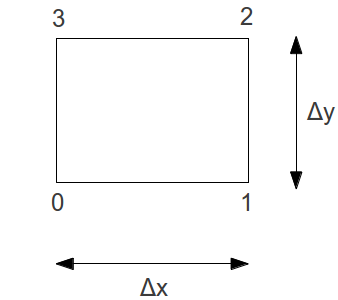
\includegraphics[width=0.2\textwidth]{./Spatial_discretizations/cell}
  \caption{Cell}
\end{figure}
are:
\begin{align}
  &\chi_0(x,y) = \frac{(\Delta x-x)}{\Delta x}\frac{(\Delta y-y)}{\Delta y}\\
  &\chi_1(x,y) = \frac{x}{\Delta x}\frac{(\Delta y-y)}{\Delta y}\\
  &\chi_2(x,y) = \frac{x}{\Delta x}\frac{y}{\Delta y}\\
  &\chi_3(x,y) = \frac{(\Delta x-x)}{\Delta x}\frac{y}{\Delta y}
\end{align}
with $x\in[0,\Delta x]$ and $y\in[0,\Delta y]$. On a square cell, the basis 
functions are given in Figure (\ref{bld}):
\begin{figure}[H]
\centering    
\subfloat[First basis function]{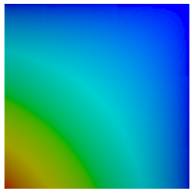
\includegraphics[width=0.25\textwidth]
  {./Spatial_discretizations/bld_1}}
\subfloat[Second basis function]{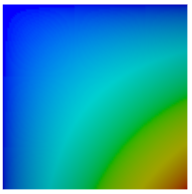
\includegraphics[width=0.25\textwidth]
  {./Spatial_discretizations/bld_2}}\\
\subfloat[Third basis function]{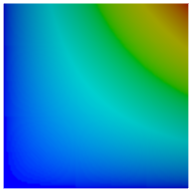
\includegraphics[width=0.25\textwidth]
  {./Spatial_discretizations/bld_3}}
\subfloat[Fourth basis function]{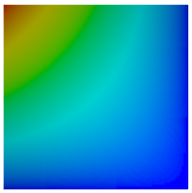
\includegraphics[width=0.25\textwidth]
  {./Spatial_discretizations/bld_4}}
\caption{BLD basis function}
\label{bld}
\end{figure}
Given these basis functions, the matrices of
\cref{element_residual_formula} (1D and 2D mass matrix, $\bs{M}_{ij} = \int_K
\chi_i \chi_j\ d\br$ and the ``gradient'' matrix, $\bs{G}_{ij} = \int_K \chi_i
\bn \chi_j\ d\br$) can be easily analytically computed on rectangular cells.
On ``almost'' rectangular cells, the integrals have to be computed
analytically. On highly distorted cells, these integrals become singular.

\subsection{PieceWise Linear Discontinuous finite elements}
Next, we introduce the PieceWise Linear Discontinuous finite
elements developed in \cite{pwld_3d,pwld_2d}. The interest of PWLD finite
elements is that they can be used on arbitrary polygons. We will see in
Chapter \ref{mip_chapter} the advantages of using arbitrary polygons instead
of triangles or quadrilaterals. To obtain the PWLD basis
functions on two-dimensional polygons, we need to introduce the within-cell
point $c$. The coordinates of $c$ are weighted averages of the vertex coordinates:
\begin{align}
& x_c = \sum_{j=1}^{N_V} \alpha_{j} x_j\\
& y_c = \sum_{j=1}^{N_V} \alpha_{j} y_j
\end{align}
where $\sum_{j=1}^{N_V} \alpha_{j}=1$, $\alpha_j \geq 0\ \forall j$, and $N_V$ is 
the number of vertices of the cell.\\
The basis function at vertex $j$ is defined by \cite{pwld_2d}:
\begin{equation}
\chi_{j} (x,y) = t_{j}(x,y) + \alpha_j t_c(x,y)
\end{equation}
where the $t_j$ function is the linear functions such that $t_j (x,y)$ is
unity at vertex $j$ and zero at the  $j-1$, $j+1$, and $c$. The function 
$t_c(x,y)$ is unity at $c$ and zero at each vertex. In this work, the arbitrary 
positive weights $\alpha_j$ are chosen to be $\frac{1}{N_V}$. On a square cell with 
$\alpha_{j}=\frac{1}{4}\ \forall j$, the basis functions are given in Figure 
(\ref{pwld}):
\begin{figure}[H]
\centering
\subfloat[First basis function]{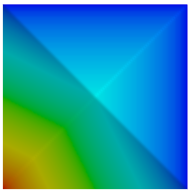
\includegraphics[width=0.25\textwidth]
  {./Spatial_discretizations/pwld_1}}
\subfloat[Second basis function]{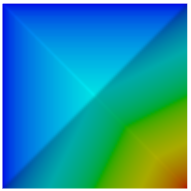
\includegraphics[width=0.25\textwidth]
  {./Spatial_discretizations/pwld_2}}\\
\subfloat[Third basis function]{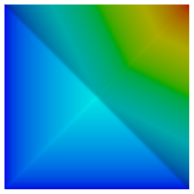
\includegraphics[width=0.25\textwidth]
  {./Spatial_discretizations/pwld_3}}
\subfloat[Fourth basis function]{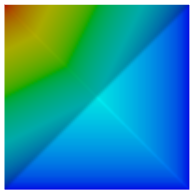
\includegraphics[width=0.25\textwidth]
  {./Spatial_discretizations/pwld_4}}
\caption{PWLD basis function}
\label{pwld}
\end{figure}
On triangular cells, the PWLD basis functions reduces to the standard Linear
Discontinuous (LD) basis functions if $\alpha_j = \frac{1}{3}$. 

Given the definition of the PWLD finite elements, it may seem complicated to
build the mass matrix, $\bs{M}$, or the gradient matrix, $\bs{G}$, on an 
arbitrary polygonal cells. The construction of such matrices can be greatly 
simplified using ``side'' sub-cells. A ``side'' sub-cell is a triangular cell 
made from two adjacent vertices and the point $c$. On each ``side'' sub-cells, 
the mass matrix, for example, can be build using LD finite elements. To do so, 
we first need to rewrite the mass matrix $\bs{M}$:
\begin{equation}
  \bs{M} = \sum_{k=1}^{N_V} \int_{S_k} \chi_i \chi_j\ d\br
\end{equation}
where $S_k$ are the ``side'' sub-cells (see Figure \ref{fig_sub_cell}). We see 
that $\bs{M}$ can be built by looping over all the ``side'' sub-cells. For a 
given ``side'' sub-cell $S_k$, we have:
\begin{equation}
  \int_{S_k} \chi_i \chi_j\ d\br = \int_{S_k} \(t_i t_j + \alpha
  t_i t_c + \alpha t_c t_i + \alpha^2 t_c^2\) d\br
\end{equation}
On $S_k$, the basis function $t_i$, $t_j$, and $t_c$, are identical to the LD
basis function. Therefore, if we note $\bs{M}_{S_k}$, the mass matrix on the 
``side'' sub-cell formed by the vertices 0, 1, and $c$:
\begin{figure}[H]
  \centering
  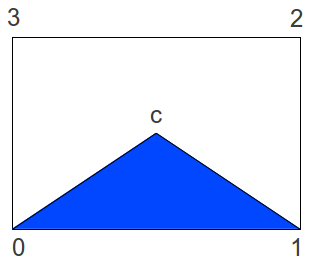
\includegraphics[width=0.3\textwidth]{./Spatial_discretizations/mass_matrix}
  \caption{Sub-cell (in blue) in the cell}
  \label{fig_sub_cell}
\end{figure}
$\bs{M}$ can be built using $\bs{M}_{S_k}$:
{\allowdisplaybreaks
\begin{align}
  & \bs{M}(0,0) =  \bs{M}_{S_k}(0,0) + \alpha \bs{M}_{S_k}(0,2) + \alpha
  \bs{M}_{S_k}(2,0) + \alpha^2 \bs{M}_{S_k}(2,2)\\
  & \bs{M}(0,1) =  \bs{M}_{S_k}(0,1) + \alpha \bs{M}_{S_k}(0,2) + \alpha
  \bs{M}_{S_k}(2,1) + \alpha^2 \bs{M}_{S_k}(2,2)\\
  & \bs{M}(0,2) =  \alpha \bs{M}_{S_k}(0,2) + \alpha^2 \bs{M}_{S_k}(2,2)\\
  & \bs{M}(0,3) =  \alpha \bs{M}_{S_k}(0,2) + \alpha^2 \bs{M}_{S_k}(2,2)\\
  & \bs{M}(1,0) =  \bs{M}_{S_k}(1,0) + \alpha \bs{M}_{S_k}(1,2) + \alpha
  \bs{M}_{S_k}(2,0) + \alpha^2 \bs{M}_{S_k}(2,2)\\
  & \bs{M}(1,1) =  \bs{M}_{S_k}(1,1) + \alpha \bs{M}_{S_k}(1,2) + \alpha
  \bs{M}_{S_k}(2,1) + \alpha^2 \bs{M}_{S_k}(2,2)\\
  & \bs{M}(1,2) =  \alpha \bs{M}_{S_k}(1,2) + \alpha^2 \bs{M}_{S_k}(2,2)\\
  & \bs{M}(1,3) =  \alpha \bs{M}_{S_k}(1,2) + \alpha^2 \bs{M}_{S_k}(2,2)\\
  & \bs{M}(2,0) =  \alpha \bs{M}_{S_k}(2,0) + \alpha^2 \bs{M}_{S_k}(2,2)\\
  & \bs{M}(2,1) =  \alpha \bs{M}_{S_k}(2,1) + \alpha^2 \bs{M}_{S_k}(2,2)\\
  & \bs{M}(2,2) =  \alpha^2 \bs{M}_{S_k}(2,2)\\
  & \bs{M}(2,3) =  \alpha^2 \bs{M}_{S_k}(2,2)\\
  & \bs{M}(3,0) =  \alpha \bs{M}_{S_k}(2,0) + \alpha^2 \bs{M}_{S_k}(2,2)\\
  & \bs{M}(3,1) =  \alpha \bs{M}_{S_k}(2,1) + \alpha^2 \bs{M}_{S_k}(2,2)\\
  & \bs{M}(3,2) =  \alpha^2 \bs{M}_{S_k}(2,2)\\
  & \bs{M}(3,3) =  \alpha^2 \bs{M}_{S_k}(2,2). 
\end{align}}    
To finish to build $\bs{M}$, we need to loop over all of the ``side''
sub-cells, $S_k$ ($k=1,\hdots,N_v$), of the cell. The gradient matrix is built 
similarly.

\section{Conclusions}
In this section, we explained how Source Iteration, Krylov solvers, and
Diffusion Synthetic Acceleration can be used to solve the transport equation. 
The two spatial discretization, BLD and PWLD finite elements, that we will 
employ in the next Chapters have been presented.



\chapter{\uppercase{Angular Multigrid Preconditioner for $S_n$ equations with Highly
Forward-Peaked Scattering Kernel}} \label{anmg_chapter}
\section{Introduction}
The discrete ordinates method has been shown to be quite accurate for electron
and coupled electron-photon transport \cite{accuracy_2,morel_81,accuracy_1}, 
which is required in the development of radiation therapy protocols, satellite 
electronics shielding, flash x-ray machine design, and a wide variety of other 
applications. Charged particles interact through Coulomb interactions with the 
background medium. Such interactions predominately result in extremely small changes 
in particle direction and energy. These interactions are well characterized by the
Fokker-Planck limit of the transport equation \cite{fp_limit,morel_96}. In this 
limit, the directional and energy changes are decoupled with the former modeled 
by the continuous scattering operator and the latter modeled by the continuous 
slowing-down operator. In this Chapter, we consider the discrete-ordinate ($S_n$) 
angular discretization of the transport equation with a focus upon iterative 
solution methods for problems with highly forward-peaked scattering characteristic 
of the Fokker-Planck limit. 

When the scattering is highly forward-peaked, solving the $S_n$ transport
equation can be challenging due to the slow convergence of the standard iterative
algorithm, Source Iteration (SI). To speed up iterative convergence,
acceleration schemes such as Diffusion Synthetic Acceleration (DSA) are used.
With isotropic or weakly anisotropic scattering, DSA is generally highly
effective \cite{dsa_ref}. This occurs because the quickly varying
error modes are strongly attenuated by the transport sweep, whereas the
diffusion operator attenuates the slowly varying error modes. However, DSA can
be completely ineffective in the Fokker-Planck limit \cite{multigrid_1d} because
the diffusion operator does not attenuate all the slowly varying error modes.

To address this deficiency, an  angular multigrid method for the
one-dimensional $S_n$
equations was developed by Morel and Manteuffel (MM) \cite{multigrid_1d}. This
method was extremely efficient yielding a maximum spectral radius for 
a model infinite-medium problem of 0.6 at a cost of
approximatively twice that of DSA. This maximum spectral radius is approached
in the Fokker-Planck limit whereas in the same limit, the spectral radius of DSA
approaches one. 

Pautz, Adams, and Morel (PAM) \cite{multigrid_2d} generalized the MM method to
2-D, but it was found to be stable only for weakly forward-peaked scattering.
The instability arose from high-frequency spatial error amplification that
occurred in the transfer of error estimates between angular grids (a sequence
of different $S_n$ orders). Stabilization was achieved by filtering the error
estimates via diffusion operators. However, this filtering was expensive and
significantly degraded the effectiveness of the method such that the spectral
radius approaches one in the Fokker-Planck limit.  Nonetheless, the method was 
always more efficient than the DSA method for the test problems considered.

In this Chapter, the PAM method with no filtering (PAMNF) is recast as a 
preconditioner and used in conjunction with the GMRES Krylov method. In this form, 
stability of the iteration scheme is guaranteed. Krylov subspace methods have been 
developed to solve large sparse linear systems. Their application to the transport 
equation has been extensively studied in the past \cite{faber,oliveira,patton,warsa} 
where the importance of preconditioning was highlighted. In \cite{oliveira}, the 
authors used successfully the 1D MM angular method as a preconditioner for GMRES 
and CGS. These preconditioned Krylov methods were significantly faster than MM. 
In this research, we compute the eigenvalues of preconditioned system for a model 
problem and compare the spectrum with those of preconditioners based upon transport 
sweeps and DSA. It is found that relative to these preconditioners, PAMNF 
preconditioning moves the eigenvalues away from zero while leaving them 
constrained to a reasonably small portion of the complex plane. These are 
desirable properties for a preconditioner because the convergence rate of GMRES 
is proportional to the size of the eigenvalue cluster and/or the distance between 
the clusters \cite{campbell,warsa}. The eigenvalues close to zero slow down the 
convergence of GMRES because they can be viewed as single values that are processed 
one at the time \cite{campbell,warsa}. We also compare the convergence rates and 
efficiency of these preconditioners for various test problems with forward-peaked 
scattering. We find that PAMNF preconditioning is significantly more efficient 
than DSA preconditioning, and becomes increasingly so as the Fokker-Planck limit 
is approached. However, unlike the MM method for one-dimensional geometries, 
the number of iterations required for convergence 
nonetheless increases as this limit is approached. In spite of this fact, 
the PAMNF-preconditioned Krylov method achieves good efficiency without the 
costly filtering associated with the original PAM fixed-point iteration scheme, 
and appears to be more effective than other existing algorithms for solving 
the $S_n$ equations with highly forward-peaked scattering.

One key feature of the angular multigrid method is that transport sweeps can
strongly damp the high frequency error modes (upper half of the flux moments)
with the use of an ``optimal'' transport correction \cite{multigrid_1d}. This
``optimal'' transport correction is a variant of the well-known extended
transport correction \cite{lathrop,morel_79}.

\section{Iterative schemes for highly forward-peaked scattering}
\subsection{Source Iteration and DSA}
\Cref{transport_operator} can be solved using the Source Iteration 
method, which is a Richardson iteration, or a Krylov method. The Source
Iteration method at the $k^{th}$ iteration is given by:
\begin{equation}
\Phi^{(k+1)} = \bs{DL}^{-1} \bs{M\Sigma}\Phi^{(k)}+\bs{DL}^{-1}Q
\end{equation}
When the scattering ratio $c=\max_{l}\(\frac{\Sigma_{s,l}}{\Sigma_t}\)$ is close
to one, the spectral radius of SI can become arbitrary close to one and the
convergence becomes arbitrary slow. Since
most physical forward-peaked scattering produces $\Sigma_{s,0} >
\Sigma_{s,1}>\hdots$, the flat modes are the ones which should be accelerated
that is why the DSA scheme is used. The SI+DSA scheme is given by a transport sweep:
\begin{equation}
\Phi^{(k+1/2)} = \bs{DL}^{-1}\bs{M\Sigma}\Phi^{(k)} +\bs{DL}^{-1}Q,
\label{dsa_sweep}
\end{equation}
followed by a diffusion synthetic acceleration for the correction:
\begin{equation}
\delta \Phi^{(k)} = \bs{\mc{T}}_0^{-1} \bs{R}_{n\rightarrow0}
\(\Phi^{(k+1/2)}-\Phi^{(k)}\),
\label{correction}
\end{equation}
yielding the next iterate for the flux moments:
\begin{equation}
\Phi^{(k+1)} = \phi^{(k+1/2)} + \bs{P}_{0/1\rightarrow n} \delta \Phi^{(k)}
\label{si_dsa_it}
\end{equation}
Finally, using \crefrange{dsa_sweep}{si_dsa_it}, we obtain:
\begin{equation}
\begin{split}
\Phi^{(k+1)} =& \((\bs{I}+\bs{P}_{0/1\rightarrow n}\bs{\mc{T}}_0^{-1} \bs{R}_{n
\rightarrow 0}\bs{DL}^{-1} \bs{M\Sigma} - \bs{P}_{0/1\rightarrow n}
\bs{\mc{T}}_0^{-1} \bs{R}_{n\rightarrow 0}\) \Phi^{(k)}\\
&+ (\bs{I} + \bs{P}_{0/1\rightarrow n}\bs{\mc{T}}_0^{-1} \bs{R}_{n\rightarrow
0}) \bs{DL}^{-1} Q.
\end{split}
\label{dsa_it}
\end{equation}
where $\bs{\mc{T}}_0$ is the matrix associated to the DSA operator,
$\bs{R}_{n\rightarrow 0}$ is the restriction matrix of $\Phi_n$ (all moments)
to $\Phi_0$ (only $0^{th}$ moment) and $\bs{P}_{0/1\rightarrow n}$ the
projection matrix of $\Phi_0$ or $\Phi_1$, depending whether only the zeroth
or the zeroth and the first moment are accelerated, onto $\Phi_n$. When only
the zeroth moment is accelerated, the scheme is always stable and the spectral
radius is max $\(\rho_{iso},\frac{\Sigma_{s,1}}{\Sigma_t}\)$ where
$\rho_{iso}$ is the spectral radius when the scattering is isotropic. In
multidimensional geometry, when both the zeroth and the first moments are
accelerated, the scheme is not always stable and the spectral radius is given
by $\(\rho_{iso},\frac{\Sigma_{s,1}}{\Sigma_{t}-\Sigma_{s,1}}\)$
\cite{multisweep}. For highly forward peaked scattering, accelerating the
zeroth moment is ineffective $\(\frac{\Sigma_{s,1}}{\Sigma_t}\rightarrow 1\)$,
whereas accelerating both moments can be unstable
$\(\frac{\Sigma_{s,1}}{\Sigma_t-\Sigma_{s,1}}>1\)$.

\section{Review of previous angular multigrid work}
\subsection{One dimensional geometry: the Morel and Manteuffel (MM) method}
As mentioned previously, only the zeroth and the first flux moments can be
accelerated with DSA. To accelerate higher moments, other methods have to be
used. Morel and Manteuffel proposed an angular multigrid method to accelerate
the SI calculation of the one-dimension $S_n$ equations with highly
anisotropic scattering \cite{multigrid_1d}. They use a variation of the
extended transport correction \cite{lathrop} to attenuate the ``upper half''
of the flux moments (higher frequencies) thanks to transport sweeps. The
``lower half'' of the flux moments (lower frequencies) is accelerated using
the $S_{n/2}$ equations. These $S_{n/2}$ equations are themselves accelerated
using $S_{n/4}$ equations. The order of the transport operator is divided
by two until the $S_4$ level. At this point, the $P_1$ equations are used to
accelerate the $S_4$ equations. For the general case where $n/2^i$ is odd, we need
to define:
\begin{equation}
Half(n) = \left\{
\begin{aligned}
&\frac{n}{2}, &\textrm{if }\frac{n}{2}\textrm{ is even}\\
&\frac{n}{2}+1, &\textrm{if }\frac{n}{2}\textrm{ is odd}
\end{aligned}
\right.
\end{equation}
Using this definition of ``Half'' to coarsen the angular grid, the sequence of
sweeps for an $S_{16}$ base level is $(S_{16}-S_8-S_4)$ and for a $S_{18}$
base level, the sequence is $(S_{18}-S_{10}-S_6-S_4)$. Morel and Manteuffel's
scheme works as follows:
\begin{enumerate}
\item Perform a transport sweep for the $S_n$ equations.
\item Perform a transport sweep for the $S_{n_2}$ equations with a $P_{n_2-1}$
expansions using the $S_n$ residual as the inhomogeneous source, where
$n_2=Half(n)$.
\item Continue coarsening the angular grid by a factor two (i.e., according to
the definition of ``Half'') until a sweep has been performed for the $S_4$
equations.
\item Solve the $P_1$ equations ($P1$ synthetic acceleration, $P1SA$) with a
$P_1$ expansion of the $S_4$ residual as the inhomogeneous source.
\item Add the Legendre moments of the $P_1$ solution to the Legendre moments
of the $S_4$ iterate to obtain the accelerated $S_4$ iterate.
\item Continue to add the corrections from each coarse grid to the finer grid
above to obtain the accelerated $S_n$ moments.
\end{enumerate}
Every time a transport sweep is performed, the optimal transport correction
needs to be used \cite{multigrid_1d}. For a $P_{n-1}$ expansion of the cross
sections, the corrected cross sections are given by:
\begin{equation}
\Sigma_{s,j}^* = \Sigma_{s,j} - \frac{\Sigma_{s,n/2}+\Sigma_{s,n-1}}{2}
\textrm{with }j=\{t\}\textrm{ or }\{s,l\}.
\end{equation}
This correction is said to be optimal because for an infinite homogeneous
medium, it minimizes the ``high-frequency'' angular errors, the smoothing
factor being given by:
\begin{equation}
\rho_s =\max\(|\Sigma_{s,n/2}|/\Sigma_{s,0},|\Sigma_{s,n/2+1}|/\Sigma_{s,0},
\hdots,|\Sigma_{s,n-1}|/\Sigma_{s,0}\).
\label{rho_s}
\end{equation}
To compare the effectiveness of the angular multigrid method with DSA,
Fokker-Planck scattering cross sections (\cref{sigma_m_sigma}) can be used. In
one dimension geometry, DSA becomes less efficient as $\Sigma_{s,l}$ $(0<l\leq
L)$ becomes closer to $\Sigma_{s,0}$. Therefore, in the limit as $L\rightarrow
\infty$, DSA no longer accelerates the convergence of SI for Fokker-Planck
scattering (the spectral radius tends to 1.0). However, the spectral radius of
the angular multigrid method has an upper bound of $0.6$ when $L\rightarrow
\infty$. It can be easily shown by using \cref{rho_s} and the fact that for
Fokker-Planck scattering cross sections the cross-section moments decrease
monotonically:
\begin{equation}
  \begin {split}
  \rho_s &= \frac{\Sigma_{s,N/2}^*}{\Sigma_{s,0}}\\
         &= \frac{3N-6}{5N-6}
  \end{split}
\end{equation}
which tends to 0.6 when $N$ goes to infinity.

The MM method converges in less iterations than DSA but it is important to
look at the cost of each MM iterations: one sweep in each $N$ directions + one
DSA iteration + one sweep in each ($\frac{N}{2}+\frac{N}{4}+\hdots$)
directions. Since $\frac{N}{2}+\frac{N}{4}+\hdots \leq N$, the cost of one MM 
iteration is less than: two sweeps in each $N$ directions + one DSA iteration.

\subsection{Multidimensional geometry: the Pautz-Adams-Morel (PAM) methods}
In the multidimensional case, DSA becomes unstable when both the zeroth and
the first flux moments are accelerated and $\frac{\Sigma_{s,1}}{\Sigma_t}\geq
0.5$, \cite{multisweep}. In \cite{multigrid_2d}, the authors modified the one
dimensional angular multigrid method by accelerating only the zeroth flux
moment with the DSA and by using $S_2$ as lowest transport sweep instead of
$S_4$. Even so, the proposed method (PAMNF, with ``NF'' for no-filtering) was
unstable and a filter was needed to stabilize the scheme (PAMF). Therefore,
the angular multigrid method was modified as follows \cite{multigrid_2d}:
\begin{enumerate}
\item Perform a transport sweep for the $S_n$ equations.
\item Perform a transport sweep for the $S_{n_2}$ equations with a $P_{n_2}$
for 2-D problem and a $P_{n_2+1}$ for 3-D problem expansion for the $S_n$
residual as the inhomogeneous source, where $n_2 = Half(n)$.
\item Continue coarsening the angular grid by a factor two (i.e., according to
the definition of ``Half'') until a sweep has been performed for the $S_2$
equations.
\item Solve the diffusion equation with a $P_0$ expansion for the $S_2$
residual as the inhomogeneous source.
\item Apply a diffusive filter to the corrections from steps 2 and 3 (without
this, the method is unstable).
\item Add the corrections from steps 4 and 5 to the Legendre moments of the
$S_n$ iterate to obtain the accelerated $S_n$ moments.
\end{enumerate}
The filter stabilizes the method which otherwise would diverge. Without the
filtering process, the low frequency are well attenuated but instabilities are
introduced in higher frequency modes. Filtering eliminates the high frequency
corrections which are well attenuated by SI alone but it keeps the low
frequency corrections. The filter is given by:
\begin{equation}
\(-\bn\cdot \frac{\beta_f}{3\Sigma_f}\bn + \Sigma_f\) f_{corr} = \Sigma_f
\(\Phi_{n_2}+P_{n_4\rightarrow n_2}\Phi_{n_4}+\hdots+P_{2\rightarrow
n_2}\Phi_2\)
\end{equation}
where $\Sigma_f$ is the filter cross section and $\beta_f$ is the filter
tuning parameter. A Fourier analysis shows that given an input amplitude $A$,
the ``diffusively filtered'' amplitude is:
\begin{equation}
F=\frac{A}{1+\frac{\beta_f \lambda^2}{3\Sigma_f}}.
\end{equation}
It is clear that the modes with large $|\lambda|$ (high frequencies) are
strongly attenuated while low-frequency are not. However, the filtering
process does not prevent the spectral radius from becoming arbitrary close to
1 when $L$ becomes large \cite{multigrid_2d}.

\section{Angular multigrid as preconditioner for Krylov Solvers}
In this research, we propose to abandon SI as the solver for the $S_n$
equations with highly-forward peaked scattering and to use a Krylov solver
instead. The DSA-preconditioned system of equations solved with a Krylov method is:
\begin{equation}
\begin{split}
&\((\bs{I} + \bs{P}_{0/1\rightarrow n} \bs{\mc{T}}_0^{-1} \bs{R}_{n\rightarrow
0})(\bs{I}-\bs{DL}^{-1}\bs{M\Sigma})\) \phi=\\
&(\bs{I}+\bs{P}_{0/1\rightarrow n} \bs{\mc{T}}_0^{-1} \bs{R}_{n\rightarrow
0})\bs{DL}^{-1} Q.
\end{split}
\end{equation}
The angular multigrid scheme can also be recast to be used by a Krylov
solver. Here, we have chosen the recast the PAM method without filtering
(PAMNF) as a preconditioner for a Krylov solver. The successive corrections of
the angular multigrid acceleration form now different stages of a
preconditioner used in the Krylov solver. Two variations of the PAMNF
preconditioner will be tested:
\begin{itemize}
\item the coarsest level is DSA (ANMG-DSA) (with the coarsest $S_n$ level
being $S_2$).
\item the coarsest level is $P1SA$ (ANMG-P1SA) (with the coarsest $S_n$ level
being $S_4$).
\end{itemize}
First, we present the angular multigrid using DSA and then, the angular
multigrid using $P1SA$. Later, these two versions are compared.
\subsection{ANMG-DSA}
Using a method similar to the one we used to write the equation for the
preconditioned Krylov solver, we recast the PAMNF for SI as a preconditioner
for a Krylov solver. First, we write the SI sweep equation, the successive
corrections and the new iterate built from the sweep values plus all the
successive corrections:
\begin{align}
& \Phi_n^{(k+1/2)} = \bs{D}_n\bs{L}_n^{-1}\bs{M}_n\bs{\Sigma}_n\Phi_n^{(k)} +
\bs{D}_n \bs{L}_n^{-1} Q\\
& \delta \Phi_{n_2}^{(k)} = \bs{D}_n\bs{L}_{n_2}^{-1} \bs{M}_{n_2}
\bs{\Sigma}_{n_2} \bs{R}_{n\rightarrow n_2}
\(\Phi_n^{(k+1/2)}-\Phi_n^{(k)}\)\\
& \hdots\\
& \delta \Phi_2^{(k)} = \bs{D}_2 \bs{L}_2^{-1} \bs{M}_2 \bs{\Sigma}_2
\bs{R}_{4\rightarrow 2}\delta \Phi_4\\
& \delta \Phi_0^{(k)} = \bs{\mc{T}}_0^{-1} \bs{R}_{2\rightarrow 0}\delta
\Phi_2^{(k)}\\
& \Phi_n^{(k+1)} = \Phi_n^{(k+1/2)} + \bs{P}_{n_2\rightarrow n} \delta
\Phi_{n_2}^{(k)} + \hdots + \bs{P}_{2\rightarrow n} \delta \Phi_2^{(k)} +
\bs{P}_{0\rightarrow n} \delta \Phi_0^{(k)}. \label{mom_update}
\end{align}
Now, all the corrections $\delta \Phi_0^{(k)}$ through $\delta \Phi_{n_2}^{k}$
are substituted into the moment update equation, \cref{mom_update}, yielding:
\begin{equation}
  \begin{split}
    \Phi_n^{(k+1)} =& \bs{T}_n \Phi_n^{(k)} + \bs{D}_n \bs{L}_n^{-1} Q +
     \bs{P}_{n_2\rightarrow n}\(\bs{T}_{n_2}\bs{R}_{n\rightarrow n_2}
     \(\Phi_n^{(k+1/2)}-\Phi_n^{(k)}\)\)+\hdots\\
     &+\bs{P}_{2\rightarrow n} \bs{T}_2\bs{R}_{4\rightarrow 2} \delta \Phi_4^{(k)}
     + \bs{P}_{0\rightarrow n} \bs{\mc{T}}_0^{-1} \bs{R}_{2\rightarrow 0} \delta
     \Phi_2^{(k)}\\
    =& \bs{T}_n\Phi_n^{(k)} + \bs{D}_n \bs{L}_n^{-1} Q + \bs{P}_{n_2\rightarrow n}
     \(\bs{T}_{n_2} \bs{R}_{n\rightarrow n_2} \(\bs{T}_n \Phi_n^{(k)} +\bs{D}_n
     \bs{L}_n^{-1} Q\right.\right.\\
     &\left.\left.-\Phi_n^{(k)}\)\)+\hdots+\bs{P}_{2\rightarrow n} \bs{T}_2 
     \bs{R}_{4\rightarrow 2}\( \bs{T}_4 \bs{R}_{8\rightarrow 4} \(\hdots\(\bs{T}_n 
     \phi_n^{(k)} + \bs{D}_n  \bs{L}_n^{-1} Q\right.\right.\right.\\
     &\left.\left.\left.-\Phi_n^{(k)}\)\)\)+ \bs{P}_{0\rightarrow n} 
     \bs{\mc{T}}_0^{-1} \bs{R}_{2\rightarrow 0}
     \(\bs{T}_2 \bs{R}_{4\rightarrow 2}\(\hdots\( \bs{T}_N\Phi_n^{(k)} + \bs{D}_n
     \bs{L}_n^{-1}Q\right.\right.\right.\\
     &\left.\left.\left.-\Phi_n^{(k)}\)\)\)\\
    =& \(\bs{T}_n + \bs{P}_{n_2\rightarrow n} \bs{T}_{n_2} \bs{R}_{n\rightarrow
     n_2} (\bs{T}_n -\bs{I}) + \hdots + \bs{P}_{2\rightarrow n} \bs{T}_2
     \bs{R}_{4\rightarrow 2}\right.\\ 
     &\left.\(\bs{T}_4 \bs{R}_{8\rightarrow 4}\(\hdots\(\bs{T}_n-\bs{I}\)\)\)+
     \bs{P}_{0\rightarrow n}\bs{\mc{T}}_0^{-1} \bs{R}_{2\rightarrow 0}
     \bs{R}_{2\rightarrow 0}\right.\\ 
     &\left. \(\bs{T}_2 \bs{R}_{4\rightarrow 2}\(\hdots\(\bs{T}_n-\bs{I}\)\)\)\) 
     \Phi_n^{(k)} + \(\bs{I}+\bs{P}_{n_2\rightarrow n}\bs{T}_{n_2} 
     \bs{R}_{n\rightarrow n_2}+ \hdots +\right.\\
     &\bs{P}_{2\rightarrow n} \bs{T}_2 \bs{R}_{4\rightarrow 2} \(\bs{T}_4
     \bs{R}_{8\rightarrow 4}\(\hdots \(\bs{T}_{n_2} \bs{R}_{n\rightarrow
     n_2}\)\)\)+\\
     &\left. \bs{P}_{0\rightarrow n} \bs{\mc{T}}_0^{-1} \bs{R}_{2\rightarrow 0}
     \(\bs{T}_2 \bs{R}_{4\rightarrow 2}\(\hdots\(\bs{T}_{n_2} \bs{R}_{n\rightarrow
     n_2}\)\)\)\) \bs{D}_n \bs{L}^{-1} Q
\end{split}
\end{equation}
where we defined $\bs{T}_n = \bs{D}_n \bs{L}_n^{-1} \bs{M}_n \bs{\Sigma}_n$
(the subscript $n$ denotes the $S_n$ level). Finally, the linear system to be
solved is given by:
\begin{align}
  &\(\bs{I}-\bs{T}_n\) \bs{P}^{MG/DSA} \xi_n = \bs{D}_n \bs{L}_n^{-1} Q
  \label{p_mg_dsa_1}\\
  &\bs{P}^{MG/DSA} \Phi_n = \xi_n \label{p_mg_dsa_2}
\end{align}
where the multigrid preconditioner $\bs{P}^{MG/DSA}$ is given by:
\begin{equation}
\begin{split}
  &\bs{P}^{MG/DSA} = \(\bs{I}+\bs{P}_{n_2\rightarrow n} \bs{T}_{n_2}
\(\bs{I}+\bs{P}_{n_4\rightarrow n_2}
\bs{T}_{n_4}\(\hdots\(\bs{I}+\bs{P}_{0\rightarrow 2}
\bs{\mc{T}}_0^{-1}\bs{R}_{2\rightarrow 0}\)\right.\right.\right.\\
&\left.\left.\left. \hdots\)\bs{R}_{n_2\rightarrow
n_4}\) \bs{R}_{n\rightarrow n_2}\).
\end{split}
\end{equation}
At this point, it is necessary to choose a DSA for implementation. Various DSA
schemes have been reviewed in \cite{dsa_ref,multisweep,trans_87,wareing,larsen_91, 
consistent_p1}. We have chosen to employ the Modified Interior Penalty
(MIP) DSA scheme developed by Wang and Ragusa \cite{mip} (see next Chapter). 
The MIP-DSA scheme is based on a discretization of the diffusion equation rather 
than the $P1$ equations. More specifically, MIP uses a bilinear \emph{discontinuous} 
trial space, which is the same trial space as the one used for the $S_n$ transport
equations. However, the MIP equations are not fully consistent with the
bilinear-discontinuous spatial discretization of the transport equation. Full
consistency requires discretization of the $P1$ equations. The consistency
discretized $P1$ equations are of a non-symmetric mixed form. The MIP-based
DSA algorithm is always stable for isotropic scattering and the MIP diffusion
matrix is symmetric positive definite (SPD), which makes it much easier to
invert than the mixed $P1SA$ equation. For instance, one can use a conjugate
gradient technique, preconditioned with SSOR to solve the MIP equation.

\subsection{ANMG-P1SA}   
Using $S_4$ as the lowest $S_n$ order followed by a $P1SA$ acceleration
(instead $S_2$ followed by DSA) in \cref{p_mg_dsa_1,p_mg_dsa_2} yields the 
following linear system:
\begin{align}
  &\(\bs{I}-\bs{T}_n\)\bs{P}^{MG/P1SA} \xi_n = \bs{D}_n\bs{L}_n^{-1} Q\\
  & \bs{P}^{MG/P1SA} \phi_n = \xi_n
\end{align}
where the multigrid preconditioner $P^{MG/P1SA}$ is now given by:
\begin{equation}
\begin{split}
&P^{MG/P1SA} = \(\bs{I}+\bs{P}_{n_2\rightarrow n} \bs{T}_{n_2}
\(\bs{I}+\bs{P}_{n_4\rightarrow n_2}
\bs{T}_{n_4}\(\hdots\(\bs{I}+\bs{P}_{1\rightarrow 4}\bs{\mc{T}}_1^{-1}
\bs{R}_{4\rightarrow 1}\)\right.\right.\right.\\
&\left.\left.\left. \hdots\)\bs{R}_{n_2\rightarrow n_4}\)
\bs{R}_{n\rightarrow n_2}\) 
\end{split}
\end{equation}
where $\bs{\mc{T}}_1$ is the matrix associated to the $P1SA$ operator. The 
$P1SA$ discretization used here is the $P1C$ method,
defined in \cite{P1C_MC2009,yaqiPhD}. This $P1SA$ preconditioner is positive
definite (PD), but not symmetric. In principle, the analytic $P1$ equations
can be put in a second-order diffusion form and discretized using the MIP
approach. However, the first moments of the angular flux will be treated with
less accuracy than the zeroth moment, which is undesirable.

\section{Eigenspectrum comparisons}
In this section, we compare the eigenvalue spectrum for a given model problem.
This is instructive because the convergence of GMRES is proportional to the
relative radii of the eigenvalue clusters and/or the maximal distance between
two clusters; furthermore, the eigenvalues close to zero are considered as
outliers that are processed one at a time and increase the asymptotic error
constant \cite{campbell}.  We use a $S_8$ Gauss-Legendre-Chebyshev Galerkin
triangular quadrature. The domain, a 5$cm-$side square uniformly discretized
using a 25 cells, is homogeneous. Fokker-Planck cross sections, with
$\alpha=1$ and $L=8$, are employed. For the spatial discretization, BiLinear
Discontinuous (BLD) finite elements are used (see next Chapter). $\Sigma_t$ 
is chosen to be equal to $\Sigma_{s,0}$. Figs. \ref{eig_sweep}-\ref{eig_anmg} 
show the eigenvalue spectrum for sweep preconditioning (Fig. \ref{eig_sweep}), 
DSA preconditioning (Fig. \ref{eig_dsa}), and angular multigrid preconditioning
(Fig. \ref{eig_anmg}). The eigenvalues were obtained using implicit QR
decomposition \cite{implicitQR}. Even though the global matrices are never
formed in transport solution techniques, we constructed them here for the
purposes of the eigenspectrum analysis (specifically, the $j^{th}$ column of
any matrix $A$ is obtained by multiplying it by the canonical basis vector
$e_j$).
\begin{figure}[H]
  \centering
  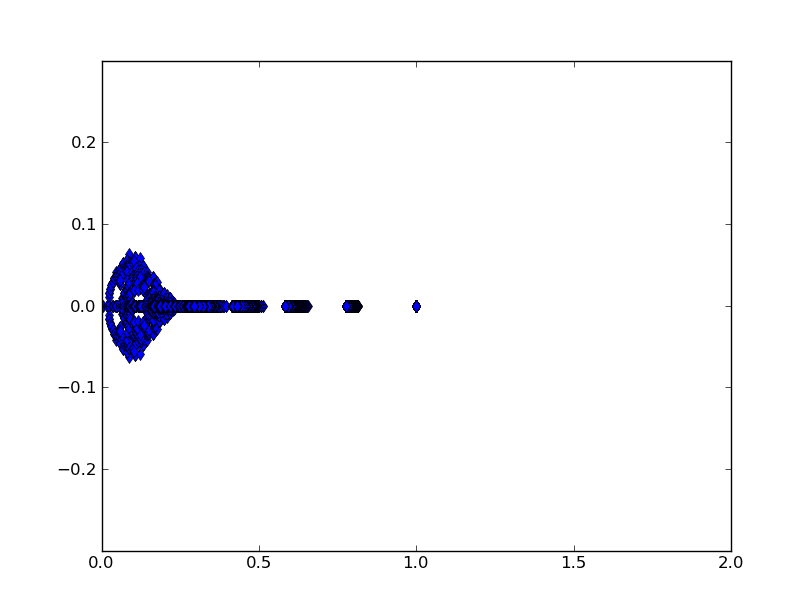
\includegraphics[width=0.5\textwidth]{./Anmg/s8_5_5}
  \caption{Eigenspectrum of the sweep preconditioned system}
  \label{eig_sweep}
\end{figure}
\begin{figure}[H]
  \centering
  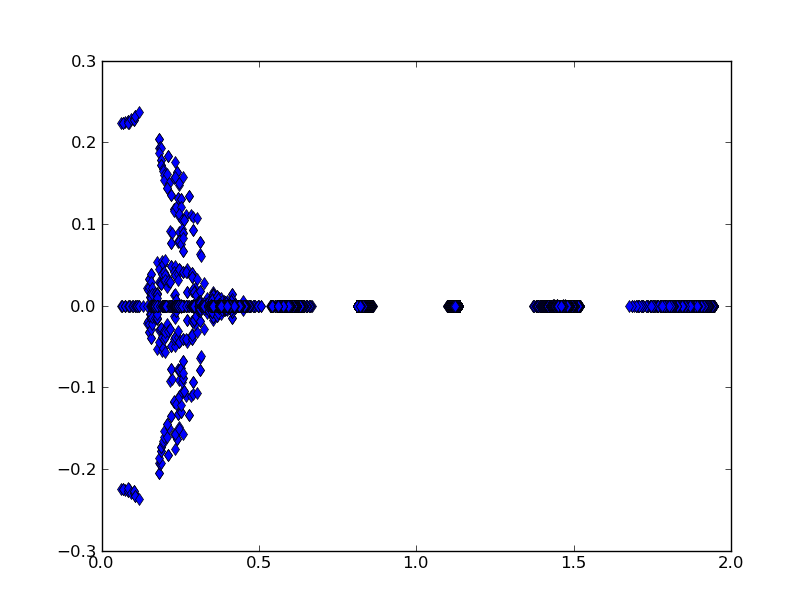
\includegraphics[width=0.5\textwidth]{./Anmg/d_s8_5_5}
  \caption{Eigenspectrum of the DSA preconditioned system}
  \label{eig_dsa}
\end{figure}
\begin{figure}[H]
  \centering
  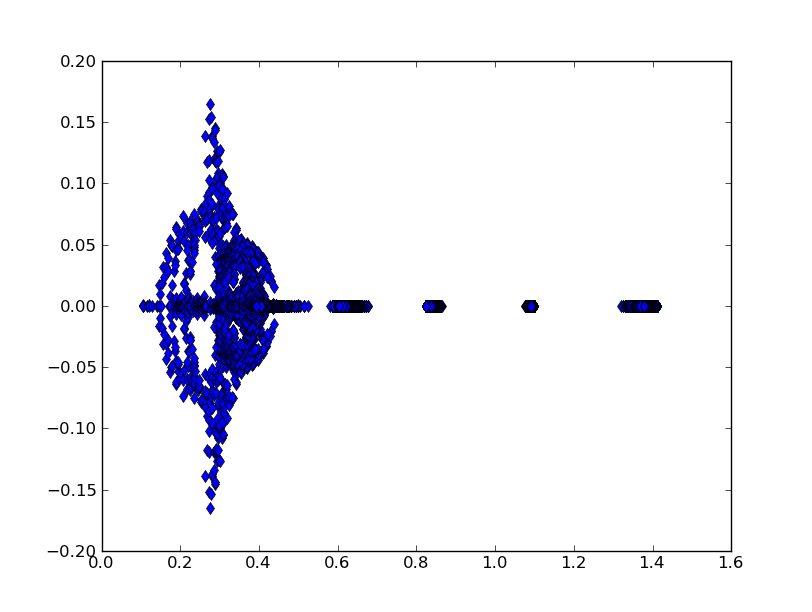
\includegraphics[width=0.5\textwidth]{./Anmg/p_s8_5_5}
  \caption{Eigenspectrum of the ANMG (DSA variant) preconditioned system}
  \label{eig_anmg}
\end{figure}
On these figures, we can note that sweep preconditioning is not effective as
many eigenvalues are located near zero. DSA moves the eigenvalues away from
zero. This explains the faster convergence of GMRES with DSA preconditioning
compared to sweep preconditioning. ANMG moves the eigenvalues even further
aways from zero than DSA and clusters them more compared to DSA. It is obvious
from these figures that ANMG preconditioning should converge much faster than
DSA preconditioning.


\section{Results}
In this section, we first compare the number of GMRES iterations needed by
ANMG-DSA and ANMG-$P1$SA to solve a model problem. Then, both the number of
GMRES iterations and the elapsed time are compared for three methods:
\begin{itemize}
  \item Sweep preconditioning (S).
  \item DSA preconditioning (DSA).
  \item Angular multigrid (DSA variant) preconditioning (ANMG-DSA).
\end{itemize}
For all the tests the first in this section, BLD finite elements are used and GMRES is
restarted every 30 iterations. For the comparison between ANMG-DSA and
ANMG-$P1$SA GMRES is restarted every 20 iterations.
\subsection{Comparison between ANMG-DSA and ANMG-$P1$SA}
The test uses a 5$cm$ square domain, uniformly discretized using $50 \times
50$ cells. The homogeneous medium is homogeneous with an uniform isotropic source of
intensity $10 n/(cm^3 s)$ and Fokker-Planck cross sections with $\alpha=1$. 
$\Sigma_t$ is chosen to be equal to $\Sigma_{s,0}$. The quadrature is the 
Gauss-Legendre-Chebyshev triangular Galerkin quadrature. The GMRES solver is 
converged to a relative tolerance, $\(\frac{\|\textrm{residual}\|_2}{\|\textrm{right 
hand side}\|_2}\)$, of $10^{-4}$. $P1$SA is solved using BiCGSTAB with a relative 
tolerance of $10^{-6}$. DSA is solved with CG preconditioned by an algebraic 
multigrid technique \cite{amg,pyamg} with a relative tolerance of $10^{-6}$. The 
number of GMRES iterations needed to solve ANMG-DSA (multigrid preconditioner 
with $S_2$ as coarsest transport level and diffusion solve) and ANMG-$P1$SA 
(multigrid preconditioner with $S_4$ as coarsest transport level and $P1$SA solve) 
are compared, see Table \ref{table_anmg_d_p1}. The comparison is performed for 
$S_4$, $S_8$ and $S_{16}$ (for which the values of the anisotropy order $L$ are 4, 
8, 16, respectively).
\begin{table}[H]
  \begin{center}
    \caption{Comparison of the number of GMRES iterations needed in ANMG-DSA
    and ANMG-$P1$SA}
    \begin{tabular}{|c|c|c|}
      \hline
      & ANMG-DSA & ANMG-$P1$SA \\
      \hline
      $S_4$ & 17 & 15 \\
      $S_8$ & 23 & 28 \\
   $S_{16}$ & 42 & 70 \\
      \hline
    \end{tabular}
  \label{table_anmg_d_p1}
  \end{center}
\end{table}
From Table \ref{table_anmg_d_p1}, it can be seen that ANMG-DSA outperforms
ANMG-$P1$SA except for $S_4$. When the anisotropy of the problem increases,
the advantage of ANMG-DSA over ANMG-$P1$SA increases. Furthermore, we note
that the $P1$SA equations are more difficult to solve (PD but non symmetric
system) than the DSA equations (which are SPD). For these reasons, we
recommend using the ANMG-DSA variant of the angular multigrid technique.
Consequently, only the ANMG-DSA method will be employed in the later tests.
\subsection{Test Case with a Volumetric Source}
In this test, we compare ANMG-DSA to Sweep and DSA preconditioning. An uniform
isotropic source of intensity 10 $n/(cm^3 s)$. $S_4$, $S_8$, $S_{16}$, and
$S_{32}$ calculations were performed. Fokker-Planck cross sections with
$\alpha=1$ are used and $\Sigma_t = \Sigma_{s,0}$. The domain is homogeneous
and its size is $50cm \times 50cm$ discretized by $50\times 50$ cells. The 
thickness of the domain varies from 50 to 2690 mean-free-path (the total cross 
section varies with $L$ for Fokker-Planck cross sections: $\Sigma_{t,S_4}=10cm^{-1},
\Sigma_{t,S_8}=36cm^{-1}, \Sigma_{t,S_{16}}=136cm^{-1}, 
\Sigma_{t,S_{32}}=528cm^{-1}$) but stays constant at five transport
mean-free-path. The relative tolerance on GMRES is $10^{-6}$ whereas the
relative convergence on DSA, solved by AGMG (see next Chapter), is $10^{-8}$.
The solution for $S_{32}$ calculation is given by:
\begin{figure}[H]
  \centering
  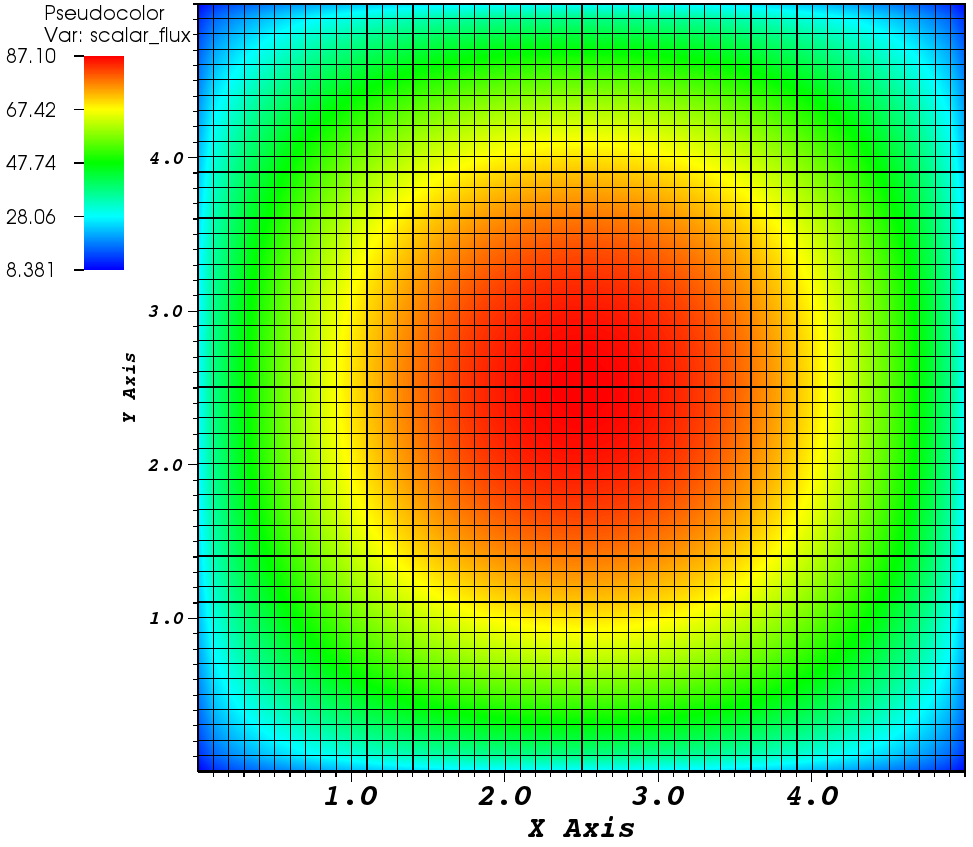
\includegraphics[width=0.6\textwidth]{Anmg/homog_anmg_crop}
  \caption{Scalar flux for the $S_{32}$ calculation.}
\end{figure}
\begin{table}[H]
  \begin{center}
    \caption{Comparison of the number of GMRES iterations needed to solve the 
      volumetric source test problem using sweep preconditioning (S), DSA 
    preconditioning, and ANMG-DSA preconditioning.}
    \begin{tabular}{|c|c|c|c|}
      \hline
      & S & DSA & ANMG-DSA \\
      \hline
      $S_4$ & 85   & 42  & 27  \\
      $S_8$ & 409  & 102 & 50  \\
   $S_{16}$ & 1530 & 266 & 105 \\
   $S_{32}$ & 4535 & 616 & 225 \\
      \hline
    \end{tabular}
    \label{table_gmres_homog}
  \end{center}
\end{table}
\begin{table}[H]
  \begin{center}
    \caption{Elapsed time (s) to solve the volumetric source test problem
      using sweep preconditioning (S), DSA preconditioning, and ANMG-DSA
    preconditioning}
    \begin{tabular}{|c|c|c|c|}
      \hline
      & S & DSA & ANMG-DSA \\
      \hline
      $S_4$ & 9.09322 & 6.51608 & 5.22796 \\
      $S_8$ & 184.949 & 52.65   & 32.7609 \\
   $S_{16}$ & 4610.94 & 740.193 & 355.939 \\
   $S_{32}$ & 138181  & 17907.9 & 7357.63 \\
      \hline
    \end{tabular}
    \label{table_time_homog}
  \end{center}
\end{table}
In Table \ref{table_gmres_homog}, one can note that ANMG-DSA always
requires the least number of iterations to converge. ANMG is the fastest
method (Table \ref{table_time_homog}). It took 38 hours to solve the $S_{32}$
problem with sweep preconditioning but only 2 hours when ANMG-DSA was used. As 
the anisotropy order is increased (i.e., increasing values of $L$ as a function 
of the number of directions in the Fokker-Planck cross-section representation), 
the advantage of ANMG-DSA is clear. The ratio $\(\frac{\textrm{number of GMRES 
iterations for ANMG-DSA}}{\textrm{number of GMRES iterations for DSA}}\)$ and
the ratio of elapsed times between the DSA and the ANMG-DSA
techniques decrease monotonically. We note from these results that
ANMG-DSA becomes increasingly superior to the standard DSA as the number of
directions becomes larger.
\subsection{Test Case with a Heterogeneous Medium (Beam problem)}
In this test, we apply a boundary source of intensity 10 $n/(cm^2 s)$ to the
entire left side of the domain $y \in [0cm,5cm]$. The top, the bottom, 
and the right boundary conditions are vacuum. The beam intensity is only 
non-zero in the most-normal directions of the quadrature. An $S_{16}$ Galerkin 
Gauss-Legendre-Chebyshev quadrature is used. The relative tolerance GMRES is
$10^{-8}$ and $10^{-10}$ for relative tolerance for DSA.The domain
is discretized using $50 \times 50$ cells and is composed of two materials:
\begin{description}
  \item[Material 1:] for $x\in [0cm,3cm]$, Fokker-Planck cross section is used with 
    $\alpha=0.099$, $\Sigma_t = 13.6 cm^{-1}$, $c=0.99$
  \item[Material 2:] for $x\in [3cm,5cm]$, Fokker-Planck cross section is used with 
    $\alpha=9.999$, $\Sigma_t = 1360 cm^{-1}$, $c=0.99$
\end{description}
Like previously, the relative tolerance on GMRES is $10^{-6}$ and the relative
tolerance on DSA is $10^{-8}$. 
\begin{figure}[H]
  \centering
  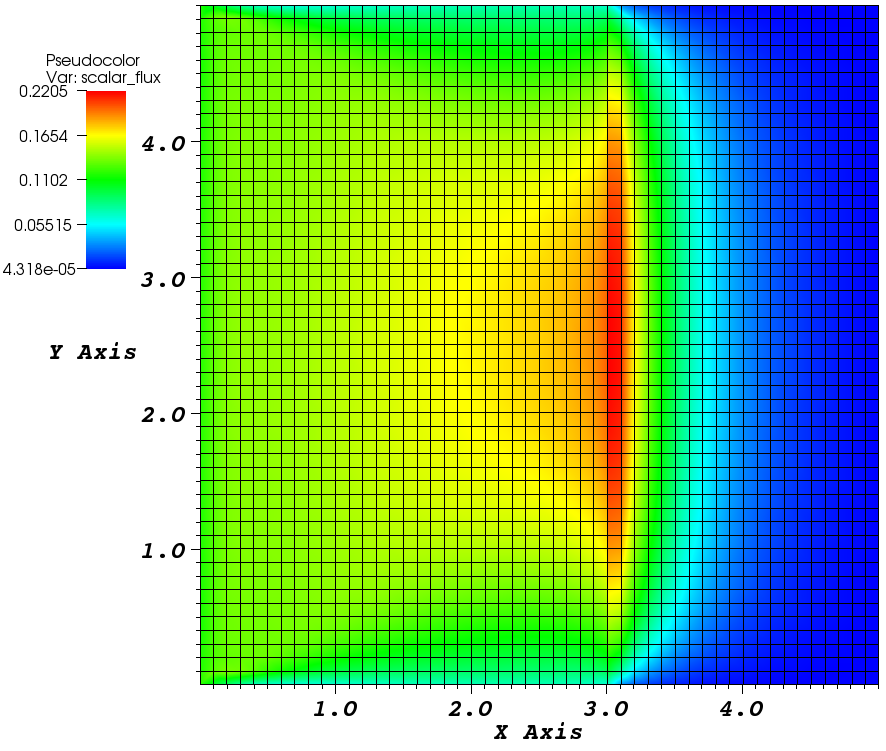
\includegraphics[width=0.6\textwidth]{Anmg/heterog_anmg_crop}
  \caption{Scalar flux for the $S_{32}$ calculation.}
\end{figure}
The number of GMRES iterations and the elapsed 
time are given in Table \ref{table_gmres_heter} and Table \ref{table_time_heter}.
\begin{table}[H]
  \begin{center}
    \caption{GMRES iterations to solve the heterogeneous problem using sweep
    preconditioning (S), DSA preconditioning, and ANMG-DSA preconditioning.}
    \begin{tabular}{|c|c|c|}
      \hline
      S & DSA & ANMG-DSA \\
      \hline
      5001 & 283 & 96 \\
      \hline
    \end{tabular}
    \label{table_gmres_heter}
  \end{center}
\end{table}
\begin{table}[H]
  \begin{center}
    \caption{Elapsed time (s) to solve the heterogeneous problem using sweep
    preconditioning (S), DSA preconditioning, and ANMG-DSA preconditioning.}
    \begin{tabular}{|c|c|c|}
      \hline
      S & DSA & ANMG-DSA \\
      \hline
      13642.8 & 897.072& 394.965 \\
      \hline
    \end{tabular}
    \label{table_time_heter}
  \end{center}
\end{table}
We can see that even on a heterogeneous medium the angular multigrid is the
most effective. The sweep preconditioning method requires a much more
iterations than DSA and ANMG-DSA preconditioning because of the Material 2
which is very thick and a scattering ratio close to one.

\section{Conclusions}
ANMG-DSA preconditioning is much more efficient than DSA preconditioning when
the scattering kernel is highly forward peaked. Unlike MM, the number of 
iterations needed to solve a problem with ANMG-DSA does not saturate as the 
anisotropy increases. However, whereas the extra work due to the additional
sweeps for MM is at most equivalent to the work done during the sweeps of a
standard iteration, the extra work for ANMG-DSA is at most a sweep on 
$\frac{n^2}{6}+n$ different directions. This number must be compared to the 
$\frac{n^2}{2}+n$ directions of a standard iteration. Thus, ANMG-DSA becomes 
cheaper compared to standard iteration as the anisotropy order increases.




\addtocontents{toc}{\protect\afterpage{\hfill{Page}\par\medskip}}
\addtocontents{toc}{\protect\afterpage{\vspace{-10pt}\hfill{}\par\medskip}}
\chapter{\uppercase{Modified Interior Penalty on Arbitrary Polygonal Cells}}
\label{mip_chapter}
\section{Introduction}
In Chapter \ref{anmg_chapter}, we noted that at the coarsest level of ANMG 
a Diffusion Synthetic Acceleration needs to be solved. 
Because analytical and closed form solutions are unavailable for most
radiation transport problems of practical interest, one typically employs
iterative techniques to solve the large system of equations that results from
the spatial and angular discretization of the transport equation. Standard
iterative techniques for the first-order form of the discrete-ordinate ($S_n$)
transport equation include the Source Iteration (SI) technique and Krylov 
subspace algorithms (usually GMRes). For highly diffusive materials (i.e., 
with scattering ratios $c=\Sigma_s / \Sigma_t $ close to 1) and optically 
thick configurations (i.e., not leakage dominated), these iterative techniques 
can become quite ineffective, requiring high iteration counts and possibly 
leading to false convergence. However, SI and GMRes-based transport solves 
can be accelerated (preconditioned) with DSA approaches 
\cite{dsa_ref,larsen_dsa,consistent_p1,m4s,wla,mip}. 

It is well established that the spatial discretization of the DSA equations
must be somewhat ``consistent'' with the one used for the $S_n$ transport equations to
yield unconditionally stable and efficient DSA schemes
(\cite{dsa_ref,larsen_dsa,consistent_p1,m4s,wla,mip}). However, 
consistency between the discretized transport equations and the discretized
diffusion may not be computationally practical (especially for unstructured
arbitrary meshes, \cite{dsa_ref}). For instance, Warsa, Wareing, and
Morel \cite{consistent_p1} derived a fully consistent DSA scheme for linear
discontinuous finite elements on unstructured tetrahedral meshes; their DSA
scheme yielded in a $P_1$ system of equations which was found to be
computationally more expensive than partially consistent DSA schemes that are
based upon discretizations of a standard diffusion equation. Some partially 
consistent schemes have been analyzed for linear discontinuous finite element
(DFE) discretizations of the transport equation on unstructured meshes, for
instance, the modified-four-step (M4S) scheme \cite{m4s}, the
Wareing-Larsen-Adams (WLA) scheme \cite{wla,wla_pwl}, and the Modified Interior
Penalty (MIP) scheme \cite{mip}.

We will come back to DSA later but first, we want to point the usefulness of
using polygonal or polyhedral cells. Such cell types may present some advantages over
traditional cells types (simplices, hexahedra) and have found some
applications in radiation transport \cite{pwld_2d,pwld_3d,cfm_dfm}. 
Some general motivations for
polyhedral cells are as follows. Simplicial cell types (triangles, tetrahedra)
can produce good  quality mesh for highly complex geometries, but are not
well suited to capture boundary layers and are prone to numerical diffusion.
Quadrilaterals and hexahedra have been shown to be less numerically diffusive
than simplicial meshes \cite{??}, but may be harder to employ for complicated
geometries. Polyhedral cells retain the attractive features of hexahedral
cells  (the number of polyhedra is often much smaller than that of tetrahedral
cells for an equivalent accuracy), while allowing for meshing
flexibility (boundary layer meshes can easily be set up, polyhedral meshes can
be generated from tetrahedral meshes, polyhedra can be included locally in
existing meshes to improve mesh quality). Meshing tools such as MSTK
\cite{mstk} and the Computational Geometry Algorithms Library \cite{cgal} may
be employed to process polyhedral meshes. For example, the radiation transport
code PDT and the CFD codes Fluent and OpenFOAM offer polyhedral mesh and
solver capabilities.

The following features of polygonal and polyhedral cells are noteworthy:
\begin{itemize}
 \item \underline{Reduced number of unknowns per cell.} To illustrate this, we
   assume one unknown per vertex in every cell, which is standard for
   transport discretizations that perform well in the thick diffusive regime.
   In the 2D hexagonal example of Figure \ref{fig_hexa_split}, the number of
   unknowns would be six (one unknown per vertex). Using triangular cells, the
   same hexagon would have to be split into four triangles at least (thus 12
   unknowns) or possibly six triangles to preserve symmetry (thus 18 unknowns in
   that case). Similarly, using quadrilateral cells, the hexagon would be
   bisected into two quadrilaterals at least (8 unknowns), but divisions into
   three or four quadrilaterals are also possible (thus, 12 or 16 unknowns).
   \begin{figure}[H]
   \centering
   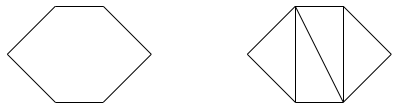
\includegraphics[width=0.5\textwidth]{./Dsa/hex_tri_cells}
   \caption{Hexagonal cell versus triangle cells.}
   \label{fig_hexa_split}
   \end{figure}
 \item \underline{Transition elements and Adaptive Mesh Refinement.} Solvers
   based on arbitrary polyhedral cells can easily handle cells with various
   numbers of edges (2D) and faces (3D). This can be particularly useful for
   simulations with Adaptive Mesh Refinement (AMR)
   \cite{amr_rad,amr_block,amr_unstruc}, without having to deal with the
   implementation of data structures to handle hanging nodes
   \cite{arbitrary_hanging_nodes,dealII_hanging_nodes,locally_hanging_nodes}.
   On Figure \ref{fig_amr}, the left cell is a pentagon whereas the two cells 
   on the right
   are quadrilaterals (a similar illustration can be made for 3D hexahedral
   AMR meshes: suppose a cell is connect to four cells through one of its faces
   - a standard situation with AMR on hexahedral grids - ; such a cell can be
   thought of as a 9-face polyhedron). Thus, a method based on a piecewise linear
   discretization can handle locally adapted meshes without any special
   treatment or further approximation of the coupling between cells.
   \begin{figure}[H]
   \centering
   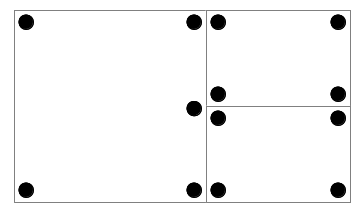
\includegraphics[width=0.3\textwidth]{./Dsa/amr}
   \caption{AMR mesh.}
   \label{fig_amr}
   \end{figure}
\end{itemize}
Several discretization methods haven been developed for 
arbitrary polygonal meshes \cite{pwld_2d,pwld_3d,cfm_dfm,pwl_diffusion,
palmer_fe,mimetic,cell_centered_diff,palmer_proc,palmer_ane,wachspress,pwbld}.
In this work, we focus on the PWLD discretization \cite{pwld_2d,pwld_3d}. This
discretization can be applied for any polygonal cells and the integrals
generated by this discretization can be easily computed analytically. 

As of today, a lot of the ongoing effort to develop a DSA scheme on
polygonal/polyhedral cells focuses on adapting the WLA scheme on polygonal meshes
\cite{cfm_dfm,wla_pwl}. The WLA scheme is a two-stage process, where first a
diffusion solution is obtained using a {\em continuous} finite element
discretization and then a {\em discontinuous } update is performed cell-by-cell 
in order to provide an appropriate discontinuous scalar flux to the DFE transport 
solver. In \cite{consistent_p1}, the WLA scheme was
found to be a stable and effective DSA technique, though its efficiency
degraded as the problem became more optically thick and highly diffusive.
To the authors' best knowledge, no work is currently done to adapt the M4S 
technique to polygonal/polyhedral meshes. This is probably due to the fact
that, even though the scheme is effective in one-dimensional slab and
two-dimensional rectangular geometries, it was found to be divergent as an
accelerator for SI in
three-dimensional tetrahedral meshes with linear discontinuous elements.
Furthermore, the scheme does not yield a Symmetric Positive Definite (SPD)
matrix. In this paper, we present an extension of the MIP technique to the
PWLD discretization techniques for for arbitrary polygonal/polyhedral meshes.
The MIP scheme is based on the standard Interior Penalty (IP) for the
discontinuous discretization of diffusion equations. MIP was first derived in
\cite{mip}, where it was applied to triangular unstructured meshes (with
locally adapted cells). MIP did not suffer the degradation of efficiency 
than WLA when the
problem becomes optically thick and highly diffusive and it is therefore an
interesting alternative to WLA. To our knowledge, this work presented the
first DSA scheme based on the same discontinuous trial spaces as the transport
finite element discretization for such meshes. Because MIP produces SPD
equations, it has been solved using conjugate gradient (CG) preconditioned by
a symmetric successive over-relaxation method (SSOR) in \cite{mip}. Here, the
effectiveness of algebraic multigrid methods (AMG) to precondition diffusion
solver \cite{amg,amg_course} will be tested and comparer with CG+SSOR.
Algebraic multigrid methods allow the use of multigrid techniques when no grid
information is available or when the grid is unstructured. Instead of using a
succession of grids based on the geometry of the problems, the ``grid levels''
are based on properties of the matrix.

\section{Modified Interior Penalty on arbitrary polygonal cells} \label{sec_mip}
First, let us recall the derivation of MIP (see \cite{mip}). MIP is based on 
the Interior Penalty (IP) form of the diffusion equation
\cite{ip,mip} (weakly imposed boundary conditions are applied to each grid
cell and the test functions are averaged over cells). The continuous equations
are :
\begin{align}
  -\bn\mathrm{D} \bn \phi_0 +\Sigma_a \phi_0 &= Q_0 & \textrm{ for }\br \in
  \mc{D}\\
  \frac{1}{4}\phi_0 - \frac{1}{2} \mathrm{D} &=0 & \textrm{ for }\br \in
  \partial \mc{D}^d\\
  -\mathrm{D}\partial_n \phi_0 &= J^{inc} & \textrm{ for }\br \in \partial
  \mc{D}^r
\end{align}
where $\phi_0$ is the scalar flux and $\mathrm{D}$ is the diffusion
coefficient. Applying the IP technique, we obtain:
\begin{equation}
  b_{IP}(\phi_0,\phi_0^*) = l_{IP}(\phi_0^*)
\end{equation}
\begin{equation}
  \begin{split}
    b_{IP}(\phi_0,\phi_0^*)=& \(\Sigma_a \phi_0,\phi_0^*\)_{\mc{D}} + 
    (\mathrm{D} \bn \phi_0, \bn \phi_0^*)_{\mc{D}} + \(\kappa_e^{IP} \llb
    \phi_0\rrb, \llb \phi_0^*\rrb\)_{E_h^i}\\
    &+ \(\llb \phi_0 \rrb,\ldb \mathrm{D} \partial_n \phi_0^*\rdb\)_{E_h^i} +
    \(\ldb \mathrm{D} \partial_n \phi_0\rdb,\llb \phi_0^* \rrb\)_{E_h^i} + 
    \(\kappa_e^{IP} \phi_0, \phi_0^*\)_{\partial \mc{D}^d}\\
    & -\frac{1}{2} \(\phi_0,\mathrm{D}\partial_n,\phi_0^*\)_{\partial \mc{D}^d}
    -\frac{1}{2}\(\mathrm{D}\partial_n\phi_0,\phi_0\)_{\partial \mc{D}^d}
  \end{split}
  \label{b_ip}
\end{equation}
and:
\begin{equation}
  l_{IP}(\phi_0^*) = \(Q_0,\phi_0^*\)_{\mc{D}} +
  \(J^{inc},\phi_0^*\)_{\partial \mc{D}^r}
\end{equation}
where $\phi_0$ and $\phi_0^*$ $\in W_{\mc{D}}^h$ where the finite
dimensional polynomial space is $W_{\mc{D}}^h = \{\phi_0 \in L^2(\mc{D});
\phi_0|_K \in V_p(K), \forall K \in \mathbb{T}_h\}$ with $V_p(K)$ is the space
of polynomials of degree up to $p$ on element $K$, $(f,g)_{\mc{D}} = 
\sum_{K\in \mathbb{T}_h} \(f,g\)_K$, 
$(f,g)_K = \int_K fg\ d\br$, $(f,g)_{E_h^i}=\sum_{e\in E_h^i}(f,g)_e$, 
$(f,g)_e = \int_e fg\ ds$, $Q_0 = \Sigma_{s,0} \delta \phi$, 
$J^{inc} = \sum_{\bo_m\cdot\bs{n}_b >0} w_m |\bo_m \cdot \bs{n}_b| \delta
\psi_m$, $\mathbb{T}_h$ is the mesh used to discretize the spatial domain
$\mc{D}$ into nonoverlapping elements $K$, $E_h^i$ is the set of interior
edges, $\partial \mc{D}^d$ is the boundary of
the domain with Dirichlet condition, $\partial \mc{D}^r$ is the boundary of
the domain with reflective condition, $\Sigma_a$ is the absorption 
cross section, D is the diffusion coefficient, $\bs{n}_b$ is the outward
normal unit vector, $\partial_n = \bs{n}_e\cdot \bn$ where $\bs{n}_e$ is the 
normal unit vector associated with a given edge $e$ (on the boundary
$\bs{n}_e = \bs{n}_b$), $\llb\phi_0\rrb = \phi_0^+ - \phi_0^-$ is the 
jump of $\phi_0$ at the interface between two elements, $\ldb\phi_0\rdb = 
\frac{\phi_0^+ + \phi_0^-}{2}$ is the mean of $\phi$ at the interface between 
two elements, $\phi_0^{\pm}=\lim_{s\rightarrow 0^{\pm}}\phi_0(\bs{r}+s\bs{n}_e)$, 
$Q_0$ represents the volumetric source term due to the successive 
error in the scattering term, and $J^{inc}$ is the incoming partial current.
The penalty parameter $\kappa_{e}^{IP}$ is given by:
\begin{equation}
  \kappa_e^{IP} = \left\{
    \begin{aligned}
      & \frac{c\(p^+\)}{2} \frac{\mathrm{D}^+}{h_{\bot}^+}+\frac{c\(p^-\)}{2}
      \frac{\mathrm{D}^-}{h_{\bot}^-}& \textrm{ on interior edges, i.e., }
      e\in E_h^i\\
      & c(p)\frac{\mathrm{D}}{h_{\bot}}& \textrm{ on boundary edges, i.e., }
      e\in \partial \mc{D}^d
    \end{aligned}
  \right.
\end{equation}
where $c(p)$ is given by $c(p)=2p(p+1)$, $p$ is the polynomial order ($p=1$ in
this research) and $h_{\bot}$ is the length of the cell in the direction
orthogonal to the edge $e$. On triangular cells, $h_{\bot}$ equals
$\frac{2A}{L_e}$ where $A$ is the area of the triangle and $L_e$ is the length
of the edge $e$.\\
This discretization of DSA is SPD. Unfortunately, the authors in \cite{mip} 
found that IP yields 
an unstable DSA scheme when the cells are large compared to the mean-free-path. 
This phenomenon is due to the fact that in optically thick medium, the ratios 
$\frac{D^{\pm}}{h^{\pm}}$ are very small. Therefore, the penalty coefficient 
is small and the method is unstable.\\
This led the authors of \cite{mip} to develop another discretization of DSA: 
the Diffusion Conforming Form (DCF). This discretization starts from 
the one-group $S_n$ transport equation with isotropic source and scattering:
\begin{equation}
  \bo_d\cdot\bn \psi_d(\br) + \Sigma_t(\br) \psi_d = \frac{1}{4\pi}
  \Sigma_s(\br) \phi_0(\br) + \frac{1}{4\pi}Q(\br)
  \label{1g_iso}
\end{equation}
The variational form of this equation is:
\begin{equation}
  b(\psi,\psi^*) = l(\psi^*)
\end{equation}
with:
\begin{equation}
  b(\psi,\psi^*) = a(\psi,\psi^*)  - \sum_{e\in \partial \mc{D}^r}
  \sum_{\bo_d\cdot \bs{n}_b<0} 4\pi w_m \la \psi_{d'},\psi_d^*\ra_e -
  \(\Sigma_s \phi_0,\phi_0^*\)_{\mc{D}}
\end{equation}
\begin{equation}
  \begin{split}
    a(\psi,\psi^*) =& \sum_{d=1}^M 4 \pi w_d \(\(\bo_d\cdot \bn +\Sigma_t\)
    \psi_d,\psi_d^*\)_{\mc{D}} + \sum_{d=1}^M 4\pi w_d \la \llb \psi_m\rrb,
    \psi_m^{*,+}\ra_{E_h^i}\\
    &+\sum_{e\in \partial \mc{D}^r} \sum_{\bo_d\cdot \bs{n}_b<0} 4 \pi\la 
    \psi_d,\psi_d^*\ra_e 
  \end{split}
\end{equation}
\begin{equation}
  l(\psi^*) = (Q,\phi^*)_\mc{D} + \sum_{e\in\partial \mc{D}^d} \sum_{\bo_d
    \cdot \bs{n}_b<0} 4\pi w_m \la \psi_m^{inc},\psi_m^*\ra_e
\end{equation}
where $\la f,g, \ra_e = \int_e |\bo_d \cdot \bs{n}_e| fg\ ds$, $\la f,g
\ra_{E_h^i} = \sum_{e\in E_h^i} \la f,g \ra_e$, and $\psi$ and $\psi^*$ 
$\in W_{\mc{D}}^h$ where the finite dimensional polynomial space is 
$W_{\mc{D}}^h = \{\psi \in L^2(\mc{D});
\psi|_K \in V_p(K), \forall K \in \mathbb{T}_h\}$ with $V_p(K)$ is the space
of polynomials of degree up to $p$ on element $K$, $(f,g)_{\mc{D}} = 
\sum_{K\in \mathbb{T}_h} \(f,g\)_K$.\\
The operator $a$ is constituted of the streaming term, the interaction term 
and the upwind terms. This is the operator that is inverted during a transport 
sweep. The operator
$b$ contains $a$, the scattering term and the reflective boundary
conditions. This operator is inverted upon convergence of SI or the Krylov solver.\\
The discretized SI at iteration $\ell$ can be written as:
\begin{equation}
  a(\psi^{(\ell+1/2)},\psi^*) = l(\psi^*) + (\Sigma_s
  \phi_0^{(\ell)},\phi_0^*)_{\mc{D}} + \sum_{e\in \mc{D}^r} \sum_{\bo_d \cdot
  \bs{n}_b < 0} 4\pi w_d \la \psi_{d'}^{(\ell)},\psi_d^*\ra_e
  \label{si_l_b}
\end{equation}
\begin{equation}
  \phi^{(\ell)} = \sum_{d=1}^M w_d \psi_d^{(\ell)}.
  \label{si_l_a}
\end{equation}
If we note the converged angular and scalar fluxes $\psi^c$ and $\phi_0^c$, we get:
\begin{equation}
  a(\psi^{c},\psi^*) = l(\psi^*) + (\Sigma_s
  \phi_0^{c},\phi_0^*)_{\mc{D}} + \sum_{e\in \mc{D}^r} \sum_{\bo_d \cdot
  \bs{n}_b < 0} 4\pi w_d \la \psi_{d'}^{c},\psi_d^*\ra_e
  \label{si_c_b}
\end{equation}
\begin{equation}
  \phi_0^{c} = \sum_{d=1}^M w_d \psi_d^{c}.
  \label{si_c_a}
\end{equation}
Subtracting \cref{si_l_a}, respectively \cref{si_l_b}, to \cref{si_c_a},
respectively \cref{si_c_b}, we obtain an angular error equation:
\begin{equation}
  a(\epsilon^{(\ell+1/2)},\psi^*) = \(\Sigma_s \mc{E}^{(\ell)},\phi_0^*\)_{\mc{D}} +
  \sum_{e\in \partial \mc{D}^r} \sum_{\bo_d \cdot \bs{n}_b<0} 4\pi w_d \la
  \epsilon_{d'}^{(\ell)},\psi_m^*\ra_e
  \label{si_f}
\end{equation}
and:
\begin{equation}
  \mc{E}^{(\ell)} = \sum_{d=1}^M w_d \epsilon_d^{(\ell)}
\end{equation}
where the angular error and the scalar error are given by:
\begin{align}
  & \epsilon^{(\ell)} = \psi^c-\psi^{(\ell)}\\
  & \mc{E}^{(\ell)} = \phi_0^c-\phi_0^{(\ell)}.
\end{align}           
It is important to note that the linear form $l$ has disappeared from
\cref{si_f} and thus, the external volumetric source and the incident
Dirichlet boundary conditions have disappeared. We now introduce:
\begin{align}
  & \delta \psi^{(\ell)} = \psi^{(\ell+1/2)}-\psi^{(\ell)} = \epsilon^{(c)}-
  \epsilon^{(l+1/2)}\\
  & \delta \phi_0^{(\ell)} = \phi_0^{(\ell+1/2)} - \phi_0^{(\ell)} = \mc{E}^{(\ell)} -
  \mc{E}^{(\ell+1/2)}.
\end{align}
Finally, we get the final form of the transport equation for the error:
\begin{equation}
  b(\epsilon^{(\ell+1/2)},\psi^*) = \(\Sigma_s \delta
  \phi_0^{(\ell)},\phi_0^*\)_{\mc{D}} + \sum_{e\in \partial \mc{D}^r} \sum_{\bo_d
  \cdot \bs{n}_b<0} 4\pi w_d \la \delta \psi_{d'}^{(\ell)},\psi_d^*\ra_e.
  \label{tsa}
\end{equation}
Note that solving \cref{tsa} would give the exact correction needed to
obtain the converged transport solution:
\begin{align}
  &\psi^c = \psi^{(\ell+1/2)} + \epsilon^{(\ell+1/2)}\\
  &\phi_0^c = \phi_0^{(\ell+1/2)} + \mc{E}^{(\ell+1/2)}
\end{align}
but solving \cref{tsa} is as difficult as solving the transport equation.
Therefore, we will replace the transport operator in \cref{tsa} by a diffusion 
operator instead. The solution of this diffusion operator will be denoted by 
a $\tilde{}$ symbol:
\begin{align}
  & \psi^{(\ell+1)} = \psi^{(\ell+1/2)} + \tilde{\epsilon}^{(\ell+1/2)}\\
  & \phi^{(\ell+1)} = \phi^{(\ell+1/2)} + \tilde{\mc{E}}^{(\ell+1/2)}
\end{align}
If we assume that the primal and dual angular fluxes
are linearly anisotropic (diffusion approximation) and we assume Fick's law to
be valid:
\begin{align}
  & \bs{J} = -\mathrm{D}\bn \phi_0\\
  & \bs{J}^* = \mathrm{D}\bn \phi_0^*,
\end{align}
we then obtain:
\begin{align}
  \tilde{\epsilon}^{(\ell+1/2)} &= \frac{1}{4\pi} (\phi_0-3\mathrm{D} \bn
  \phi_0 \cdot \bo_d) \label{eps_tilde}\\
  \tilde{\psi}_d^* &= \frac{1}{4\pi} (\phi_0^*+3\mathrm{D} \bo \phi_0^*\cdot
  \bo_d) \label{psi_tilde}
\end{align}
Substituting \cref{eps_tilde,psi_tilde} in \cref{tsa}, we obtain a
synthetic discontinuous finite elements diffusion operator in which the
scalar flux $\phi_0$ is the only unknown. Using:
\begin{align}
  & \sum_{d=1}^M w_d = 4 \pi \label{omega_0}\\
  & \sum_{d=1}^M w_d \bo_d = 0 \label{omega_1}\\
  & \sum_{d=1}^M w_d \bo_d \cdot \bo_d = \frac{4\pi}{3}\bs{I},
  \label{omega_2}
\end{align}
we obtain:
\begin{equation}
  \sum_{d=1}^M 4 \pi w_d \(\Sigma_t \tilde{\epsilon}_d^{(\ell+1/2)},
  \tilde{\psi}_d^*\)_{\mc{D}} = \(\Sigma_t \phi_0,\phi_0^*\)_{\mc{D}} -
  \(3\Sigma_t \mathrm{D} \bn \phi_0,\mathrm{D} \bn \phi_0^*\)_{\mc{D}}
\end{equation}
\begin{equation}
  \(\Sigma_s \tilde{\mc{E}}^{(\ell+1/2)},\tilde{\phi}^*\)_{\mc{D}} =
  \(\Sigma_s \phi_0,\phi_0^*\)_{\mc{D}}.
\end{equation}
If we define:
\begin{equation}
  \mathrm{D} = \frac{1}{3\Sigma_t}
\end{equation}
we get:
\begin{equation}
  \begin{split}
    & \sum_{d=1}^M 4 \pi w_d \(\Sigma_t \tilde{\epsilon}_d^{(\ell+1/2)},
    \tilde{\psi}_d^*\)_{\mc{D}} + \(\Sigma_s \tilde{\mc{E}}^{(\ell+1/2)},
    \tilde{\phi}^*\)_{\mc{D}} = \(\Sigma_a \phi_0,\phi_0^*\)_{\mc{D}} -\\
    &\(\bn \phi_0, \mathrm{D} \bn \phi_0^*\)_{\mc{D}}.
  \end{split}
\end{equation}
Now, we analyze the streaming term:
\begin{equation}
  \begin{split}
    \sum_{d=1}^M 4 \pi w_d \(\bo_d \cdot \bn \tilde{\epsilon}_d^{(\ell+1/2)},
    \tilde{\psi}_d^*\)_{\mc{D}}  =& \(\bn \phi_0,\mathrm{D} \bn
    \phi_0^*\)_{\mc{D}} - \(\bn \cdot \mathrm{D} \bn
    \phi_0,\phi_0^*\)_{\mc{D}}\\
    =& \(\bn \phi_0, \mathrm{D} \bn \phi_0^*\)_{\mc{D}} - \(\bn \cdot \bn
    \phi_0,\phi_0^*\)_{\mc{D}}\\
    =& \(\bn \phi_0,\mathrm{D} \bn \phi_0^*\)_{\mc{D}} + \(\mathrm{D} \bn
    \phi_0,\bn \phi_0^*\)_{\mc{D}}\\
     & + \(\mathrm{D} \bn \phi_0^+ \cdot \bs{n}_e, 
    \phi_0^{*,+}\)_{E_h^i}\\ 
     & - \(\mathrm{D} \bo \phi_0^{-} \cdot \bs{n}_e,
    \phi_0^{*,-}\)_{E_h^i}\\
     & - \(\mathrm{D}\bn \phi_0 \cdot \bs{n_e},\phi_0^*\)_{\partial \mc{D}}
  \end{split}
\end{equation}
where integration by part was performed and we used:
\begin{equation}
  \sum_{d=1}^M w_d \bo_d \cdot \bo_d \cdot \bo_d = 0.
\end{equation}
Manipulating the interior edge terms give successively :
\begin{equation}
  \begin{split}
    \sum_{d=1}^M 4 \pi w_d \la \llb \tilde{\epsilon}_d^{(\ell+1/2)}\rrb,
    \tilde{\psi}_d^{*,+}\ra_{E_h^i} =& \sum_{e \in E_h^i} \sum_{d=1}^M 4 \pi
    w_d |\bo_d \cdot \bs{n}_e| \(\llb \tilde{\epsilon}_m^{(\ell+1/2)}\rrb,
    \tilde{\psi}_d^{*,+}\)_e\\
    =& \sum_{e \in E_h^i} \Bigg(\sum_{\bo_d \cdot \bs{n}_e>0} \frac{w_d}{4\pi}
    |\bo_d \cdot \bs{n}_e| \big(\llb\phi_0\rrb - 3\\ 
    &\llb \mathrm{D} \bn \phi_0\rrb \cdot \bo_d, 
    \phi_0^{*,+} + 3 \mathrm{D} \bn  \phi_0^{*+} \cdot \bo_d\big)_e -\\
    &\sum_{\bo_d \cdot \bs{n}_e<0} \frac{w_d}{4\pi} |\bo_d \cdot
    \bs{n}_e| \bigg(\llb \phi_0 \rrb - 3 \llb \mathrm{D}\bn \phi_0 \rrb\cdot
    \bo_d,\\
    &\phi_0^{*,-} +3 \mathrm{D} \bn \phi_0^{*,-} \cdot \bo_d \bigg)_e\Bigg)\\
    = & \sum_{e\in E_h^i} \sum_{\bo_d \cdot \bs{n}_e>0} \frac{w_d}{4\pi}
    |\bo_d \cdot \bs{n}_e| \(\(\llb \phi_0 \rrb - 3 \llb \mathrm{D} \bn 
    \phi_0 \rrb \cdot\right.\right.\\
    &\left. \left. \bo_d,\phi_0^{*,+} + 3 \mathrm{D} \bn \phi_0^{*,+}\cdot \bo_d\)_e -
    \(\llb \phi_0 \rrb + 3\right.\right.\\ 
    &\left.\left. \llb \mathrm{D} \bn \phi_0 \rrb \cdot \bo_d,
    \phi_0^{*,-} - 3 \mathrm{D} \bn \phi_0^{*,-} \cdot \bo_d\)_e\)\\
    =&\frac{1}{4} \(\llb \phi_0\rrb,\llb \phi_0^* \rrb\)_{E_h^i} + \(\llb
    \phi_0 \rrb,\ldb \mathrm{D} \bn \phi_0^* \cdot \bs{n}\rdb \)_{E_h^i}\\
    &-\(\llb \mathrm{D} \bn \phi_0 \cdot \bs{n}\rrb,\ldb \phi_0^*
    \rdb\)_{E_h^i} -\frac{9}{16} \(\llb \mathrm{D} \bn \phi_0\rrb,\right.\\
    &\left.  \llb \mathrm{D} \bn \phi_0^*\rrb\)_{E_h^i}
    - \frac{9}{16} \( \llb \mathrm{D} \bn \phi_0 \cdot \bs{n}\rrb,\right.\\
    &\left.\llb \mathrm{D} \bn \phi_0^* \cdot \bs{n}\rrb\)_{E_h^i}
  \end{split}
\end{equation}
where we employed the following properties of the angular quadrature:
\begin{align}
  & \sum_{\bo_d \cdot \bs{n}>0} w_d |\bo_d \cdot \bs{n}| \approx \pi \\
  & \sum_{\bo_d\cdot \bs{n}>0} w_d |\bo_d \cdot \bs{n}| \bo_d \approx
  \frac{2\pi}{3} \bs{n}\\
  & \sum_{\bo_d \cdot \bs{n}>0} w_d |\bo_d\cdot \bs{n}|\bo_m\cdot \bo_d
  \approx \frac{\pi}{4}\(\bs{I}+\bs{n}\bs{n}\)
\end{align}
where $\bs{n}\bs{n}$ is a matrix. Even if these properties cannot be strictly
satisfied, numerical results show that the error is negligible.
Finally, we obtain:
\begin{equation}
  b_{DCF}(\phi_0,\phi_0^*) = l_{DCF}(\phi_0^*)
\end{equation}
with:
\begin{equation}
  \begin{split}
    b_{DCF}(\phi_0,\phi_0^*)=& \(\Sigma_a \phi_0,\phi_0^*\)_{\mc{D}} +
    \(\mathrm{D}\bn \phi_0,\mathrm{D}\bn \phi_0\)_{\mc{D}} + \frac{1}{4} 
    \(\llb\phi_0\rrb,\llb\phi_0^*\rrb\)_{E_h^i}\\
    & + \(\llb \phi_0\rrb, \ldb\mathrm{D}\partial_n 
    \phi_0^*\rdb\)_{E_h^i} + \(\ldb\mathrm{D} \partial_n \phi_0\rdb, \llb
    \phi_0^*\rrb\)_{E_h^i}\\
    & + \frac{1}{4} \(\phi_0,\phi_0^*\)_{\partial \mc{D}^d} -\frac{1}{2}
    \(\phi_0,\mathrm{D} \partial_n \phi_0^*\)_{\partial \mc{D}^d}\\
    & - \frac{1}{2} \(\mathrm{D} \partial_n \phi_0,\phi_0\)_{\partial
    \mc{D}^d}-\frac{9}{16} \(\llb\mathrm{D}\bn\phi_0\rrb,\llb\mathrm{D} \bn
    \phi_0^*\rrb\)_{E_h^i}\\ 
    &- \frac{9}{16}\(\llb\mathrm{D}\partial_n \phi_0\rrb,\llb 
    \mathrm{D}\partial_n \phi_0^*\rrb \)_{E_h^i}-\frac{9}{16} 
    \(\mathrm{D}\bn \phi_0,\mathrm{D}\bn \phi_0^*\)_{\partial \mc{D}^d}\\
    & - \frac{9}{16} \(\mathrm{D}\partial_n
    \phi_0,\mathrm{D} \partial_n \phi_0^*\)_{\partial \mc{D}^d}
    -\frac{9}{4}\(\mathrm{D}\partial_n \phi_0,\mathrm{D}\partial_n
    \phi_0^*\)_{\partial \mc{D}^r}
  \end{split}
\end{equation}
\begin{equation}
  \begin{split}
    l_{DCF}(\phi_0^*) =& \(Q_0,\phi_0^*\)_{\mc{D}}+\(
     J^{inc},\phi_0^*\)_{\partial \mc{D}^r} - \(\bs{\mc{Y}},\mathrm{D}\bn
    \phi_0^*\)_{\partial \mc{D}^r}\\ 
    &+ 2 \(\bs{\mc{Y}}^{inc} \cdot \bs{n}, \mathrm{D} \partial_n 
    \phi_0^*\)_{\partial \mc{D}^r}
  \end{split}
\end{equation}
where $\bs{\mc{Y}}^{inc} = - \sum_{\bo_d \cdot \bs{n}_b>0} 3 w_d \bo_d |\bo_d
\cdot \bs{n}_b| \delta \psi_d^{(\ell)}$.\\
DCF is symmetric but not positive definite positive. DCF is unstable for cell size
in between one and four mean-free-paths but it is stable and very efficient 
for optically thick medium. In this case, $\bn \phi_0 \approx 0$ and 
$\partial_n \phi_0 \approx 0$ and the terms $\(\mathrm{D} \bo
\phi_0^{\pm},\mathrm{D}\bn\phi_0^{*,\pm}\)$ and $\(\mathrm{D} \partial_n
\phi_0^{\pm},\mathrm{D}\partial_n \phi_0^{\pm}\)$ are negligible.
In this limit, $b_{DCF}$ becomes:
\begin{equation}
  \begin{split}
    b_{DCF}(\phi_0,\phi_0^*)=& \(\Sigma_a \phi_0,\phi_0^*\)_{\mc{D}} +
    \(\mathrm{D}\bn \phi_0,\mathrm{D}\bn \phi_0\)_{\mc{D}}
    +\frac{1}{4}\(\llb\phi_0\rrb,\llb\phi_0^*\rrb\)_{E_h^i}\\
    &+ \(\llb \phi_0\rrb, \ldb\mathrm{D}\partial_n \phi_0^*\rdb\)_{E_h^i} +
    \(\ldb\mathrm{D} \partial_n \phi_0\rdb, \llb \phi_0^*\rrb\)_{E_h^i}
    + \frac{1}{4} \(\phi_0,\phi_0^*\)_{\partial \mc{D}^d}\\ 
    &-\frac{1}{2} \(\phi_0,\mathrm{D} \partial_n \phi_0^*\)_{\partial \mc{D}^d} -
    \frac{1}{2} \(\mathrm{D} \partial_n \phi_0,\phi_0\)_{\partial
    \mc{D}^d}
  \end{split}
\end{equation}
which is exactly the same equation than \cref{b_ip} if 
$\kappa_e^{IP}=\frac{1}{4}$.\\
MIP is obtained by replacing the penalty coefficient, $\kappa_e^{IP}$, 
by $\kappa_e^{MIP}=\max \(\kappa_e^{IP},\frac{1}{4}\)$ in \cref{b_ip}.
This ensures that MIP will converge in optically thick medium since the
penalty coefficient will never be less than $\frac{1}{4}$.

DSA gives only a correction for the scalar flux but by assuming that the angular 
dependence satisfies a diffusion expansion, the angular correction can be 
computed using \cref{eps_tilde}. 
This correction can be used when some of the boundary 
conditions are periodic or reflective.

If PWLD finite elements are used instead of LD finite elements, the weak form 
of MIP is not modified. However when the cells are not triangular, there is no 
simple way to compute $h_{\bot}$. To simplify this, we assume that the polygonal 
cells are not too far from being regular polygonal 
cells. In such cases, if the cell has an even number of edges, the orthogonal 
length equals two times the apothem, i.e. two times the segment between the 
midpoint of a side of the polygon and the center of this polygon 
$\(\textrm{apothem}=2\times \frac{\textrm{area}}{\textrm{perimeter}}\)$. If 
the cell has an odd number of edges, the orthogonal length is given by the 
apothem plus the circumradius, i.e. the radius of the circle circumscribed to 
the polygon $\(\textrm{circumradius}=\sqrt{\frac{2\times \textrm{area}}{V
\sin\(\frac{2\pi}{V}\)}}\)$. Therefore, $h_{\bot}$ is given by:
\begin{table}[H]
\begin{center}
\caption{Orthogonal length of the cell for different cells}
\begin{tabular}{|c|c|c|c|c|}
\hline
Number of edges & 3 & 4 & $> 4$ and even & $> 4$ and odd \\
\hline
$h_{\bot}$ & $2 \times \frac{\textrm{area}}{L_e}$ &
$\frac{\textrm{area}}{L_e}$ & $4\times
\frac{\textrm{area}}{\textrm{perimeter}}$ & $2 \times
\frac{\textrm{area}}{\textrm{perimeter}}+\sqrt{\frac{2\times
\textrm{area}}{V\sin\(\frac{2\pi}{V}\)}}$\\
\hline
\end{tabular}
\end{center}
\end{table}

\section{Algebraic Multigrid} \label{sec_amg}
\subsection{Introduction}
As mentioned earlier, the most common way to solve a SPD system is to use
conjugate gradient preconditioned with SSOR (PCG-SSOR). In this research, we
will compare the calculation time using PCG-SGS, which is PCG-SSOR with a
damping factor equals to unity, with the time needed by CG 
preconditioned with an algebraic multigrid method. This is not a new idea: the 
first multigrid methods developed were geometric multigrid used as stand-alone 
solvers. In many applications, they achieve the so-called ``textbook multigrid
efficiency'', i.e. ``the solution to the governing system of equations [is
attained] in a computational work that is a small multiple of the operation
counts associated with discretizing the system'' \cite{textbook_eff}. However, 
in many other applications, multigrid methods, and particularly algebraic 
multigrid methods, cannot achieve such efficiency \cite{k_cycle}. In
such cases, they are often used as preconditioner for Krylov subspace methods. 
AMG make  very good preconditioners because they reduce all the error modes. Of
course, some modes may not be accelerated which can significantly degrades the 
efficiency of AMG as preconditioner. In \cite{amg_pn}, the authors used an 
algebraic multigrid method to precondition the Krylov solver for the even-parity 
finite element-spherical harmonics (FE-$P_N$) method. The AMG preconditioner 
resulted in a 60\% reduction in the solution time compared to ILU(0) 
preconditioning and even more reduction compared to SSOR preconditioning. 

We will employ and compare two multigrid approaches: one from the ML package
\cite{ml_guide} from the Trilinos library and the AGMG code \cite{agmg_guide}. 
ML is a multigrid preconditioning package that uses a smoothed aggregation 
algebraic multigrid to build a preconditioner for a Krylov method. AGMG is an 
aggregation-based algebraic multigrid code (written in Fortran 90).

We describe the multigrid principles, using first a two-grid setting. Consider
the following system:
\begin{equation}
  \bs{A}_f u_f = b_f
\end{equation}
defined on the fine grid $\mathbb{T}_f$.  The two-grid algorithm is given by :
\begin{enumerate}
  \item Perform $\nu_1$ pre-smoothing iterations using a smoother (e.g., Jacobi,
    Gauss-Seidel or ILU) using an initial guess $u_0$: $u = S^{\nu_1}(u_0,b_f)$
  \item Compute the residual on the fine grid $\mathbb{T}_f$ and restrict it to
    the coarse grid $\mathbb{T}_c$: $r_c = \bs{R}(b_f-\bs{A}_f u)$
  \item Solve with a direct solver the system on the coarse grid: 
    $v=\bs{A}_c^{-1} r_c$
  \item Interpolate the coarse grid correction to the fine grid and add the
    correction to $u$: $u \leftarrow u+\bs{P}v$
  \item Perform $\nu_2$ post-smoothing iterations: $u = S^{\nu_2}(u,b_f)$
\end{enumerate}
When using AMG, the matrix $\bs{A}_c$ on the coarse grid is given by the Galerkin
approximation:
\begin{equation}
  \bs{A}_c = \bs{R}\bs{A}_f \bs{P},
\end{equation}
where $\bs{P}$ is a prolongation matrix and $\bs{R}$ is a restriction matrix.
Solving the system $\bs{A}_c v = r_c$ on the coarse grid is generally very
expansive, therefore this step is recursively replaced by $\gamma$
applications of the  two-grid
methods until the system can be efficiently inverted with a direct solver.
This yields the multigrid method. When $\gamma = 1$, respectively $\gamma =
2$, the multigrid method is said to use a $V-$cycle, respectively a $W-$cycle:
\begin{figure}[H]
  \centering
  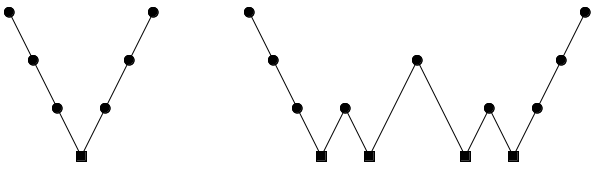
\includegraphics[width=0.5\textwidth]{./Dsa/v_w_cycles}
  \caption{$V-$ and $W-$cycles}
\end{figure}
A dot represents a smoothing operation and a square a direct inversion. The grid 
transfer operators are symbolized by lines.

For the coarsening step, both geometric and algebraic multigrid methods are 
based on the concept of smooth error. The difference between the two methods 
is that for geometric multigrid method, after the smoothing step, the error 
is \emph{geometrically} smooth relative to the coarse grid \cite{review_amg}. 
For algebraic multigrid methods, there might not be any grid and thus, only 
the properties of the matrix can be used. Therefore, the geometrical smoothness 
of the error cannot be used anymore. In fact, after the smoothing step, the 
error may be not smooth at all from the geometrical point of view. The reason 
is that the error is considered smooth when the smoother does not change the 
solution significantly anymore \cite{amg_course}:
\begin{equation}
  \|Se\|_{\mc{H}} \approx \|e\|_{\mc{H}}
\end{equation}
where $S$ is the smoother, $e$ is the error, and $\|u\|_{\mc{H}} =
\sqrt{(u,u)_{\mc{H}}}$ is the norm associated to the scalar product:
\begin{equation}
  (u,v)_{\mc{H}} = \(\bs{A}u,v\)_2.
\end{equation}
Among the algebraic multigrid methods, there are three main different 
types: the classical Ruge-Stueben AMG (also known as interpolation method), 
the plain aggregation AMG, and the smoothed aggregation AMG. ML uses 
smoothed aggregation AMG and AGMG uses plain aggregation AMG. The difference 
between theses methods is the coarsening step. The coarsening step is the 
most important step because if the coarsening is too fast, the convergence 
rates will decrease. However, if the coarsening is too slow, a lot of memory 
may be required to solve the problem. For classical Ruge-Stueben methods, 
each variable of the coarse grid is also a variable in the fine grid whereas 
for the aggregation methods, the variables of the fine grid are aggregates in
variables of the coarse grid. There is no simple identification between the 
variables of the fine grid and the coarse grid. However, all the algebraic
multigrid methods uses the  very important concept of strongly dependent
variables \cite{amg}:
{\definition{Given a threshold value of $0 \leq \theta \leq 1$, the variable
  $u_i$ strongly depends on the variable $u_j$ if:
  \begin{equation}
    -a_{ij} \geq \theta \max_{k \neq i} \(-a_{ik}\)
  \end{equation}}}
$a_{ij}$ must be of the same order of magnitude than the largest
off-diagonal in equation $i$ or $j$. A related definition is:
{\definition{If the variable $u_i$ strongly depends on the variable $u_j$,
then the variable $u_j$ strongly influences the variable $u_i$.}}\\
The idea behind the strong dependence is that if the coefficient $a_{ij}$ is
large, then a small change in the $j^{th}$ variable will have an important
effect on the $i^{th}$ variable. Thus, it is probably a good idea to use the
$j^{th}$ variable to interpolate the $i^{th}$ variable or to couple these two
variables in an aggregate. This can be easily seen using the concept of
smoothed error. For the error to be considered to be smoothed, assuming that
$\bs{A}$ is a $M$-matrix, i.e., off-diagonal entries of the matrix are less 
than or equal to zero and the real parts of the eigenvalues of the matrix 
are positive, the following relationship needs to be satisfied for most $i$ 
\cite{amg}:
\begin{equation}
  \sum_{j\neq i} \(\frac{|a_{ij}|}{a_{ii}}\) \(\frac{e_i-e_j}{e_i}\)^2 \ll 1
  \label{ineq}
\end{equation}
where $e_i$ is the error associated to the variable $i$. Since the left side 
of \cref{ineq} is positive, all the products must be small which means that 
at least one of the two terms of each product has to be small. When the
$i^{th}$ variable strongly depends on the $j^{th}$ variable 
$\frac{|a_{ij}|}{a_{ii}} \approx 1$, $e_i-e_j$ must be small
or equivalently $e_i \approx e_j$. This means that the error varies slowly
in the direction of strong connection. That is the reason why the coarsening
is done along these directions.

\subsection{Classical AMG (interpolation method)}
For classical AMG, the variables of the coarse grid are a subset of the
variables of the fine grid. The variables can be split in two disjoint
sets: $C$ that contains all the coarse variables and $F$ that contains all the
other variables. Thus, the error on the fine grid is given by \cite{review_amg}:
\begin{equation}
  e_{c,i} = (\bs{P} e_f)_i = \left\{
  \begin{aligned}
    & e_{c,i} & \textrm{ if } i\in C\\
    & \sum_{k\in B_i} w_{ik} e_{c,k} & \textrm{ if } i\in F
  \end{aligned}
  \right.
\end{equation}
where $B_i$ is a subset of $C$ whose variables are called interpolatory
variables. $B_i$ should be a small subset of $C$ to keep $\bs{A}_c$ sparse.
Now, we assume that $\bs{A}$ is a $M$-matrix and we review two typical 
interpolation methods:
\begin{description}
  \item[Direct interpolation:] First, we define the neighborhood of the
    $i^{th}$ as the set $N_i = \{ j \in C \cup F: j\neq i, a_{ij} \neq 0\}$.
    After the smoothing step, we can write locally:
    \begin{equation}
      e_i \approx -\frac{\(\sum_{j\in N_i} a_{ij} e_j\)}{a_{ii}}.
      \label{e_locally}
    \end{equation}
    If $B_i$ contains the variables which are strongly dependent on the
    $i^{th}$ variables, we have:
    \begin{equation}
      \frac{1}{\sum_{k\in B_i} a_{ik}} \sum_{k \in B_i} a_{ik} e_k \approx 
      \frac{1}{\sum_{j\in N_i} a_{ij}} \sum_{j \in N_i} a_{ij} e_j.
    \end{equation}
    Using this relation and \cref{e_locally}, we get the following formula for
    the weights of the interpolation:
    \begin{equation}
      w_{ik} = -\alpha_i \frac{a_{ik}}{a_{ii}}
    \end{equation}
    where $\alpha_i = \frac{\sum_{j\in N_i} a_{ij}}{\sum_{l \in B_i} a_{il}}$.
    Therefore, it is important that when the coarse variables are chosen,  
    that every variable in $F$ has enough strongly coupled
    variables in $C$ that are part of of $B_i$. If some of the off-diagonal
    entries are positive, the same development can be done as long as these
    positive terms are small, i.e., variables are not strongly coupled because
    of these terms. If the positive entries are large, the algebraically
    smooth error can oscillate. This can happen, for elliptic PDE, when 
    high-order finite elements are used or with bilinear elements on 
    quadrilateral meshes with large aspect ratios. This will negatively affect
    the performance of AMG.
  \item[More complex interpolations:] More complex interpolation schemes can
    be created but they reduce the sparsity of $\bs{P}$ and $\bs{R}$, increasing the
    size of $\bs{A}_c$. Moreover, the weakly-dependent variables will be 
    associated to smaller weights which makes them having a small effect. It
    can therefore be interesting to ignore the smallest values in the
    interpolation matrix and to rescale the others weights so that the sum of
    the weights does not change. This can slow down the convergence of the
    method but it will not make it diverge \cite{review_amg}.
\end{description}
A good rule, when coarsening the grid, is to try to have the set of coarse 
variables to form a maximally independent set, i.e. a maximal set where the 
coarse variables are not strongly coupled to each others, and the variables 
in $F$ are surrounded by the variables in $C$. We call $B_i^S$ the set of all 
strongly connected neighbors of $u_i$:
\begin{equation}
  B_i^s = \{ v_j \in B_i | -a_{ij} \geq \theta \max_{k\neq i}(-a_{i,k})\}.
\end{equation}
The interpolatory nodes $C_i$ are:
\begin{equation}
  C_i = B_i^s \cap C.
\end{equation}
Adding variables in $C_i$ increases the quality of the interpolation but
it diminishes the sparsity of the interpolation matrix and increases the
size of $\bs{A}_c$ which increases the computational cost of the method.
Thus, we want that for every variable $u_i$ in $F$, every $u_j \in B_i^s$
should be in $C_i$ or strongly connected to at least one variable in
$C_i$. This rule will make sure that the interpolation is of a good enough
quality. We also want $C$ to be a maximal subset of the variables such that 
the variables in $C$ are not strongly connected to each others. This ensures 
that the coarsening is fast enough.

\subsection{Smoothed aggregation: the ML package}
In a similar way than for the classical AMG, the smoothed aggregation
method uses the concept of strong connections. The theory for plain
aggregation method showed that the convergence bound depends of the number
of levels \cite{amg_unstruc}. This is a major flaw of the plain aggregation
method which was also observed in practice. To counter this, the smoothed
aggregation was created. This method converges fast for a lot of different 
problems including the ones with anisotropic and discontinuous coefficients.
  
When using a smoothed aggregation scheme, the smoothed interpolation operators,
$\bs{P}_k$, are the transpose of the coarsening operators,
$\bs{R}_k=\bs{P}_k^T$. Therefore, when the $\bs{P}_k$ are built, the
coarsening is known. First, the graph of the matrix is constructed: if the element
$(i,j)$ or $(j,i)$ of the matrix is non-zero, an edge is built between the
vertex $i$ and the vertex $j$ \cite{ml_guide}. Second, the vertices are
aggregated. When using ML on a single processor, two aggregation schemes can
be used: the uncoupled scheme or the maximally independent sets (MIS) scheme. 
The uncoupled scheme attempts at building aggregates of size $3^d$ where $d$ is the
dimension of the problem. The algorithm works as follows \cite{mis}:
\begin{description}
  \item[Step 1:] As long as there are points not adjacent to an aggregate:
    \begin{enumerate}
      \item Choose a point which is not adjacent to an aggregate. This point
        is a new root point.
      \item Define a new aggregate as the root point and its neighbors.
    \end{enumerate}
  \item[Step 2:] Add all the points left to the existing aggregates or form a
    new aggregates with them.
\end{description}
The MIS scheme used in ML applied the MIS algorithm of \cite{graph_coloring} to
the graph produced by the matrix $\bs{A}^2$. These two coarsening 
schemes use a fixed ratio of coarsening between levels. Once the aggregation is 
done, a tentative prolongator matrix, $\bs{\tilde{P}}_k$ is constructed 
\cite{mis}. A example of $\bs{\tilde{P}}_k$ is given by:
\begin{equation}
  \bs{\tilde{P}}_k(i,j) = \left\{
  \begin{aligned}
    &1 &\textrm{if }i^{th}\textrm{ point is contained in }j^{th}\textrm{
    aggregate}\\
    & 0 &\textrm{otherwise}
  \end{aligned}
  \right.
\end{equation}
This tentative prolongator could be used as prolongator but smoothing it
allows to have a more robust scheme. Let $\bs{S}_k$ be a smoother, for example
damped Jacobi, then the prolongator matrix is given by:
\begin{equation}
  \bs{P}_k = \bs{S}_k \bs{\tilde{P}}_k.
\end{equation}

Like for classical AMG, it can be interesting to ignore small values in
the graph since the smoother will be ineffective for the weakly coupled
variables. In ML, there is a drop tolerance, $tol$, that is used to ignore
entries in the graph if $|a_{ij}| \leq tol\ \sqrt{|a_{ij} a_{jj}|}$. The
tolerance, whose default value is zero, can be changed.  In ML, when the 
matrix is SPD, CG is used to determine the Jacobi damping parameter, which 
is an approximation of the spectral radius.

By default, the coarsening is stopped when the number of variables is less 
or equal than 128.

\subsection{Plain aggregation: the AGMG code}
Unlike ML, in AGMG the prolongator is not smoothed which results in a
cheaper setup and a decrease of required memory \cite{agmg2}. However, 
the scheme could be less robust. To counteract this weakness, 
the aggregation scheme is more complicated. Coarsening algorithms that control
the size of the aggregates tends to produce a few badly shaped aggregates.
Since the convergence of AMG is bounded by the worst aggregate, even a small 
number of badly shaped aggregates can have a huge impact on the convergence. 
In AGMG, the aggregation algorithm has as input the upper bound of the 
two-grid condition number $\bar{\kappa}_{TG}$. When the aggregates are constructed,
their quality is checked. Obviously, this increases the cost of the coarsening
and it is important that the coarsening is fast enough. Since the algorithm 
does not control the size of the aggregates, it is difficult to control the 
speed of the coarsening. However, controlling the condition number is much 
more interesting than controlling the coarsening speed. If the algorithm 
controls the condition number, it will not create bad aggregates but instead, it 
may create a few aggregates with a size below the target size but this 
does not affect the efficiency of the method in a noticeable way \cite{agmg2}. 

In AGMG, the aggregation is done by a few passes of a pairwise aggregation 
algorithm. This allows the computation of the aggregate quality to remain very 
simple and to keep the cost per iteration low. The advantage of controlling the 
condition number becomes even more important when a $K-$cycle or Krylov-cycle is 
used instead of the more common $V-$ or $W-$cycles. The difference between the 
$K-$cycle and the $V-$ or $W-$cycle is that the $K-$cycle uses recursively a 
few iterations of a Krylov solver preconditioned by a coarser grid to solve 
the coarse grid problem in the two-grid algorithm \cite{k_cycle}. This scheme 
is nonlinear and requires, when the system is SPD, to use flexible CG 
\cite{fcg_2,fcg_3,fcg_4,fcg} as Krylov solver. The advantage of the $K-$cycle is 
an increased robustness compared to $V-$ and $W-$cycle. Even when the condition 
number of the two-grid method is large, the convergence properties of the 
$K-$cycle can be independent of the number of levels \cite{k_cycle}. The 
computational cost of $K-$cycle is about the same than the cost of the 
$W-$cycle. If the number of unknowns does not decrease sufficiently from one 
level to the next, the $K-$cycle at one level is replaced by a $V-$cycle at 
this same level. The idea of $K-$cycle is not new since it was already used 
in Algebraic MultiLevel Iteration (AMLI) methods \cite{amli}. AMLI are 
hierarchical basis methods stabilized by the recursive calls of preconditioner 
created thanks to a coarse level. 

Next, we explain the coarsening step in AGMG for $M-$matrix (SPD). 
We want to create nonempty disjoint sets $G_k$, $k=1,\hdots,n_c$ called 
aggregates with each one of them associated to a variable in a coarser grid. 
Some of the unknowns are not associated to any variables in the coarse grid 
and they are in the set $G_0$. The prolongation matrix is given by:
\begin{equation}
  \bs{P}_{ij} = \left\{
    \begin{aligned}
      1& \textrm{ if }i\in G_j\\
      0& \textrm{ otherwise}
    \end{aligned}
    \right.
\end{equation}
Thus, $\bs{P}$ has at most one non-zeros entry by row. A row is only
composed of zeros if the variable associated to this row is in $G_0$. A
simple method to form the high quality aggregates of a given size would be
to test all the possibility. For an obvious reason, this cannot be done in
practise. Instead, in AGMG several passes of pairwise aggregation are done. 
The reason is that when two variables are aggregated, the quality factor of 
the aggregate $\kappa(G)$ is given by: 
\begin{equation}
  \kappa(\{i,j\}) = \frac{-a_{ij} +\(\frac{1}{a_{ii}+s_i+2a_{ij}}+
  \frac{1}{a_{jj}+s_j+2 a_{ij}}\)^{-1}}{-a_{ij}+\(\frac{1}{a_{ii}-s_i}+
  \frac{1}{a_{jj}-s_j}\)^{-1}}
\end{equation}
where $s_i = - \sum_{j\neq i} a_{ij}$. $\kappa$ is only given by the
off-diagonal entry connecting these two unknowns, their respective diagonal
entries, and the sum of all off-diagonal elements in the corresponding rows.
As $|G|$ increases, it becomes more and more costly to compute
$\kappa(|G|)$. However, checking that $\kappa(|G|)$ is below a given
threshold $\bar{\kappa}_{TG}$ is relatively cheap. It is sufficient to
check that:
\begin{equation}
  \bar{\kappa}_{TG} \bs{A}_G - \bs{M}_G\(\bs{I}-\bs{1}_G \(\bs{1}_G^T
  \bs{M}_G\bs{1}_G\)^{-1}\bs{1}_G^T\bs{M}_G\)
\end{equation}
is nonnegative definite. This can be done in $\mc{O}(|G|^3)$ operation
by verifying that the Cholesky factorization exists, i.e., there is no negative
pivot. Therefore, $\kappa(|G|)$ does not need to be computed explicitly to
make sure that $\kappa(|G|) \leq \bar{\kappa}_{TG}$. The first pairwise
coarsening step is given by:
\begin{enumerate}
  \item Create the set $G_0$, i.e., create the set of variables which will
    not be aggregated.
  \item Choose an unknown and find among its unassigned neighbors the one
    that gives the smallest $\kappa(\{i,j\})$.
  \item Check that $\kappa(\{i,j\}) \leq \bar{\kappa}_{TG}$. If the
    condition is not verified, the variable is left unassociated in the coarse
    grid.
\end{enumerate}
To increase the size of the aggregates, the temporary coarse grid matrix
$\bs{\tilde{A}}_c$ is computed and the same process that the one we just
described is applied. The set $G_0$ cannot be changed and the quality factor
$\tilde{\kappa}(\{i,j\})$ needs to be adapted to reflect the quality of the
corresponding aggregate $\kappa(G_i\cup G_j)$ in the original matrix.
Therefore, the definition of $s_j$ is slightly modified:
\begin{equation}
  \tilde{s}_i = - \sum_{k \in G_i} \sum_{j \in G_i} a_{kj}.
\end{equation}
This change is there to ensure that $\tilde{\kappa}(\{i,j\})$ is a lower
bound of $\kappa(G_i \cup G_j)$. Thus, if $\tilde{\kappa}(\{i,j\}) \geq
\bar{\kappa}_{TG}$, the pair has to be rejected because it is impossible for
$\kappa(G_i \cup G_j)$ to satisfy the condition. An unique characteristic 
of this coarsening method is that you can, in theory, have an 
arbitrary number of pairwise coarsening passes without degrading the upper
bound of the condition number. In practise, however, the coarsening is
stopped if either a given number of passes has been done or the coarsening
factor has reached a target value. To conclude the explanation of the
coarsening step, we explain how unknowns are picked and how to pick between 
a pair $\{i,j\}$ and another $\{i,k\}$ if they have the same quality factor. 
If there is no priority rules, the coarsening would depend of the ordering 
of the variables or the way off-diagonal entries are stored. In AGMG, the 
rule chosen tries to increase the regularity of the aggregates because in 
practise, this increases the coarsening speed of the coarser levels. Even 
if the coarsening step tries to create regular aggregates on regular grids, 
the results are still quite good for unstructured grids \cite{agmg2}. The 
priority rule consists of using a Cuthill-McKee permutation 
\cite{cmk} to renumber the variables and to use the number associated to the 
variable as a priority number (the lower number has the priority). The 
Cuthill-McKee permutation works as follows: the number 1 is given to a node 
with minimal degree; the next numbers are given to its neighbors ordered by
increasing degree; then their neighbors are given a number by
increasing degree; the process is over when all nodes are numbered. There is
still some uncertainties in the numbering if there are several variables
with minimal degree or when several neighbors of a variables have the same
degree. However, these choices do not affect the
performance \cite{agmg2}. 

AGMG stops the coarsening when the number of variables is less or equal to
400.

\section{Results} \label{sec_res}
In this section, we show two Fourier analysis of MIP: one where the $S_n$ order is
varied and one where the aspect ratio is varied. We also compare different
methods to solve MIP: congugate gradient (CG), conjugate gradient
preconditioned with symmetric Gauss-Seidel (PCG-SGS), conjugate gradient
preconditioned with ML using uncoupled aggregation (PCG-ML-Uncoupled),
conjugate gradient preconditioned with ML using mis aggregation (PCG-ML-MIS),
and AGMG. The options used for ML can be found in the Appendix.
\subsection{Fourier Analysis}
Analysing Source Iteration accelerated with DSA is often performed using
Fourier analysis \cite{larsen_dsa,consistent_p1}. When a Fourier analysis is
performed, the error is decomposed into different modes and by inspecting the 
damping of the different error modes, the effectiveness of the DSA scheme can 
be studied. The largest damping factor is the spectral radius of the method. 
The smaller the spectral radius is, the faster the scheme converges. If the 
spectral radius is greater than one, the method is unstable. 
\subsubsection{$S_n$ order varied}
This Fourier analysis was carried on a square cell, using a
Gauss-Legendre-Chebyshev (GLC) quadrature. The medium is homogeneous, the scattering
ratio $c=0.9999$ and periodic boundary conditions are used. The $x-$axis is the mesh
size in mean free path and the $y-$axis is the spectral radius. There are four
curves corresponding to different $S_n$ order: $S_2$, $S_4$, $S_8$ and
$S_{16}$.
\begin{figure}[H]
\centering
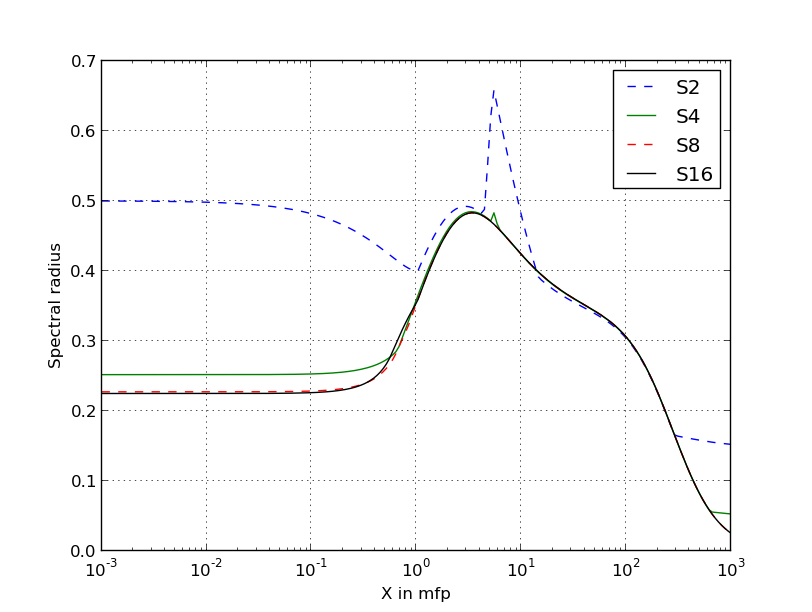
\includegraphics[width=0.5\textwidth]{./Dsa/sn_order_9999}
\caption{Fourier analysis as a function of the mesh optical thickness,
homogeneous infinite medium case.}
\end{figure}
MIP is stable for every cell size. The spectral radius is always less than
0.5, except for $S_2$ where it peaks at about 0.7.
\subsubsection{Aspect ratio varied}
For this Fourier analysis, we use a $S_{16}$ GLC quadrature, a homogeneous
medium, $c=0.9999$ and periodic boundary conditions. The $x-$axis is the mesh
size in mean free path in the $x$ direction and the $y-$axis is the spectral
radius. There are five curves corresponding to five different aspect ratio:
$\frac{Y}{X}=\frac{1}{16}$, $\frac{Y}{X}=\frac{1}{4}$, $\frac{Y}{X}=1$,
$\frac{Y}{X}=4$ and $\frac{Y}{X}=16$. 
\begin{figure}[H]
\centering
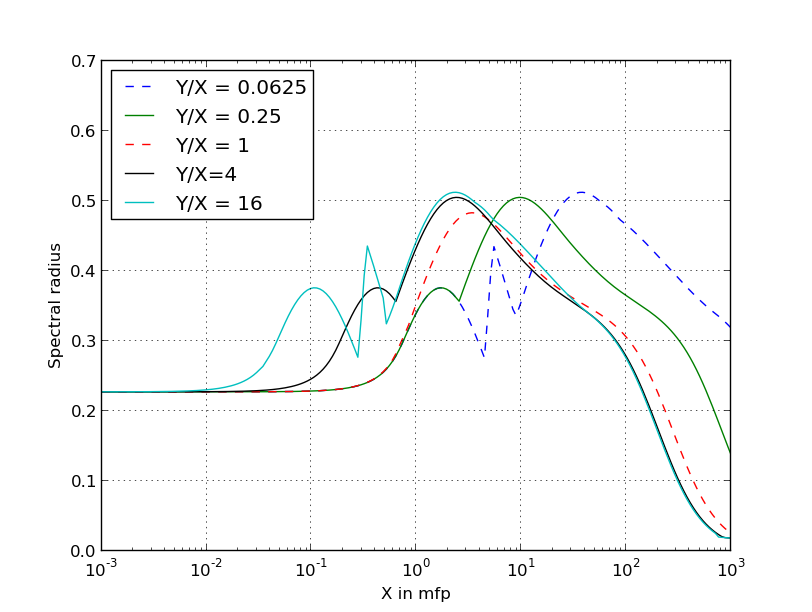
\includegraphics[width=0.5\textwidth]{./Dsa/aspect_ratio_9999}
\caption{Fourier analysis as a function of the mesh optical thickness,
homogeneous infinite medium case for different aspect ratios.}
\end{figure}
MIP is stable for every aspect ratio and the maximum of the spectral radius
peaks at about 0.5

\subsection{Homogeneous medium}
Next, we compare different solvers for MIP on a homogeneous medium, 10cm $\times$
10cm, $\Sigma_t=1$cm$^{-1}$ and $\Sigma_s=0.99$cm$^{-1}$, with vacuum boundary 
conditions and a source of intensity 1cm$^{-3}$s$^{-1}$. We use a $S_8$
Gauss-Legendre-Chebyshev quadrature, a Source Iteration solver with relative
tolerance of $10^{-8}$ and a relative tolerance for MIP of $10^{-10}$.
\subsubsection{Quadrilateral cells}
In this example, the mesh is composed of 9990 quadrilateral cells that corresponds 
to 39960 degrees of freedom. The solution is:
\begin{figure}[H]
\centering
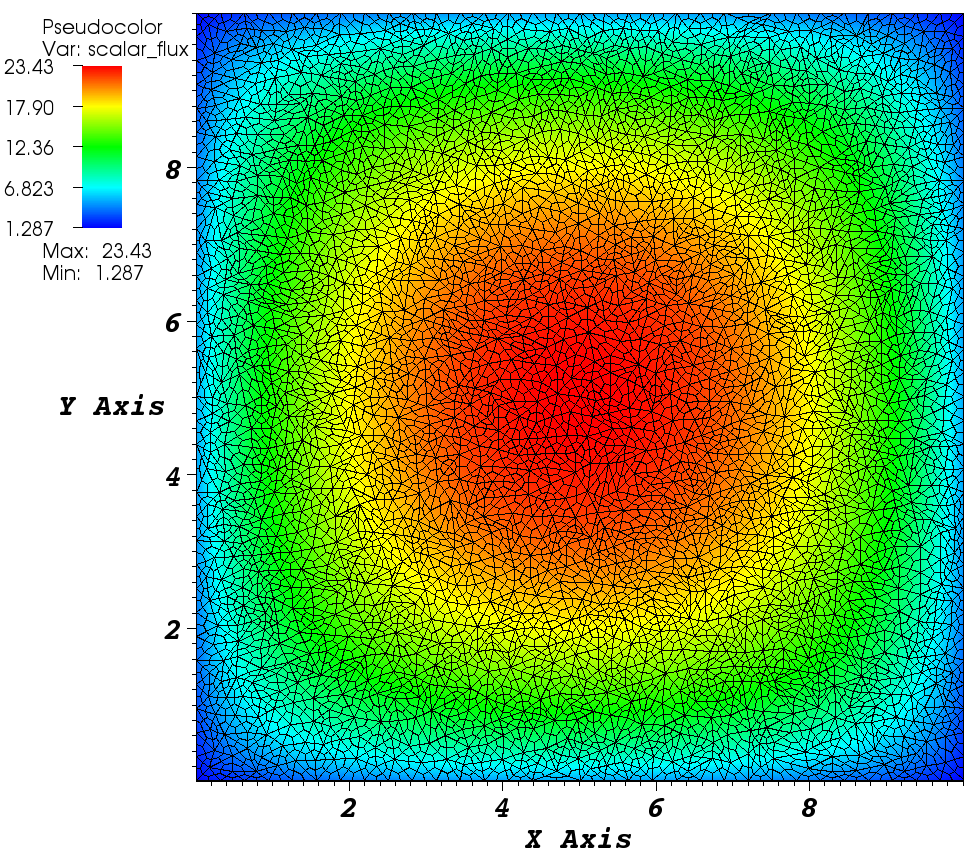
\includegraphics[width=0.6\textwidth]{./Dsa/homog_quad_crop}
\caption{Scalar flux on a mesh composed of quadrilateral cells.}
\end{figure}
In the next table, the different solvers are compared:
\begin{table}[H]
\begin{center}
\caption{Comparison of different preconditioners for quadrilateral cells.}
\begin{tabular}{|c|c|c|c|c|c|c|}
\hline
 & No-DSA & CG & PCG-SGS & PCG-MLU & PCG-MLM & AGMG\\
\hline
SI iter & 268 & 27 & 27 & 27 & 27 & 27 \\
Prec (s) & NA & NA & 0.0142572 & 0.381872 & 1.21095 & 0.068\\
MIP (s) & NA & 138.379 & 177.556 & 46.1957 & 44.7837 & 6.9311\\
CG iter & NA & 35419 & 11414 & 729 & 702 & 674\\
Total (s) & 309.395 & 172.181 & 211.933 & 80.1548 & 80.0387 &
40.827\\
\hline
\end{tabular}
\end{center}
\end{table}
In this Table, SI iter is the number iteration of Source Iteration
needed to solve the problem, Prec is the time in seconds needed to
initialize the preconditioner used by CG, MIP is the total time in
seconds spent solving DSA during the calculation, CG iter is the total number 
of CG iterations used to solve MIP, and Total is the time in
seconds needed to solve the problem.

Using MIP decreases significantly the number of SI iterations and the
calculation time as expected. Using PCG-SGS decreases by a factor three the 
number of CG iterations compared to CG but the time needed to solve MIP is
greater. With ML, the number of CG iterations is reduced by a factor 50 and 
the MIP calculation time is divided by three compared to CG. AGMG is by far 
the most efficient solver, the number of CG iteration is slightly lower 
than PCG-ML but the MIP calculation is 20 times faster than CG.

\subsubsection{Polygonal cells}
In this problem the mesh is composed of 13654 triangles, 250 quadrilaterals,
1400 pentagons, 1306 hexagons, 228 heptagons, and 6 octagons, for a total of
16844 cells and 58442 degrees of freedoms. This example will allow us to test
MIP and the different preconditioners on a mesh composed of different types of
cell. The solution and the mesh are:
\begin{figure}[H]
\centering
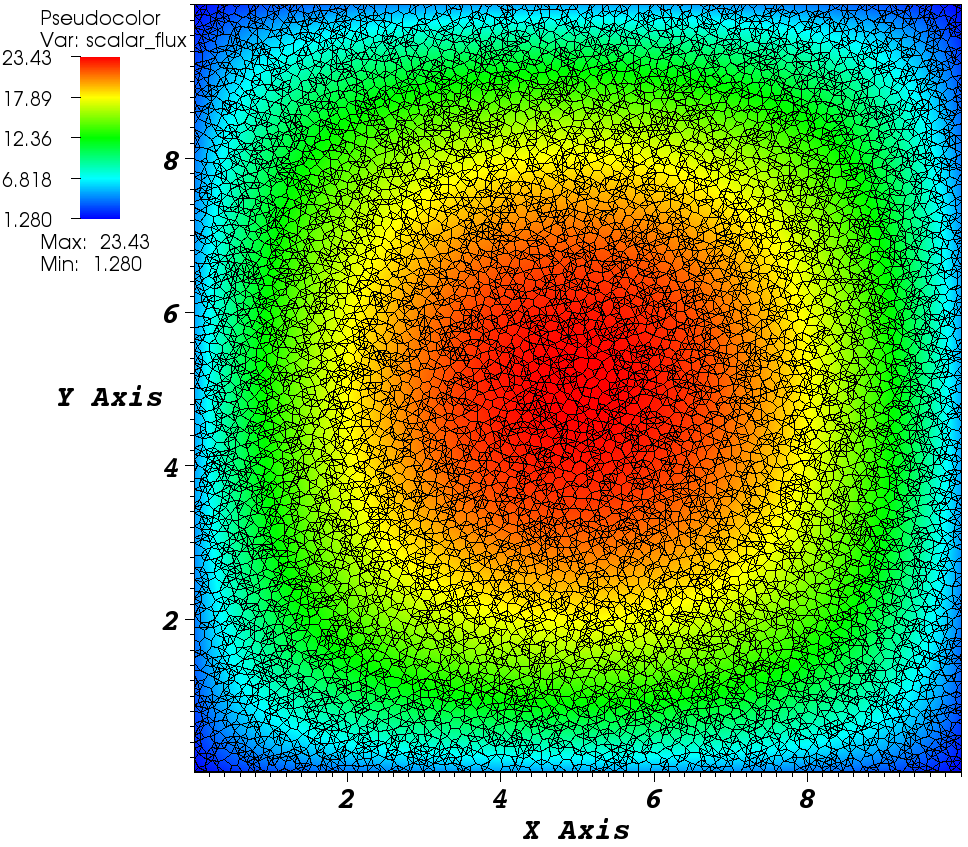
\includegraphics[width=0.6\textwidth]{./Dsa/homog_poly_crop}
\caption{Scalar flux on a mesh composed of polygonal cells.}
\end{figure}
The different solvers are compared in the next Table:
\begin{table}[H]
\begin{center}
\caption{Comparison of different preconditioners for polygonal cells.}
\begin{tabular}{|c|c|c|c|c|c|c|}
\hline
 & No-DSA & CG & PCG-SGS & PCG-MLU & PCG-MLM & AGMG\\
\hline
SI iter & 268 & 27 & 27 & 27 & 27 & 27\\
Prec (s) & NA & NA & 0.0201421 & 0.482845 & 2.09054 & 0.097\\
MIP (s) & NA & 210.128 & 303.423 & 78.0993 & 71.4493 & 11.0419\\
CG iter & NA & 36352 & 13370 & 840 & 784 & 674\\
Total (s) & 458.132 & 265.026 & 358.745 & 134.434 & 128.731 & 66.0207\\
\hline
\end{tabular}
\end{center}
\end{table}
We see that using different types of cells in the same mesh does not affect
the performance of MIP or of the preconditioners. 

\subsection{Heterogeneous medium}
In this example, we use a heterogeneous medium composed of 184 triangles, 3720
quadrilaterals and 2791 regular hexagons of side 0.05$cm$ for a total of 6695 
cells and 32178 degrees of freedom. The domain is 5.28275$cm$ by 4.6$cm$. 
Reflective boundary conditions are used. The quadrature is a $S_{16}$ 
Gauss-Legendre-Chebyshev quadrature. The SI solver has a relative tolerance of 
$10^{-8}$ and the relative tolerance for MIP is $10^{-10}$. The domain is 
composed of three zones:
\begin{figure}[H]
\centering
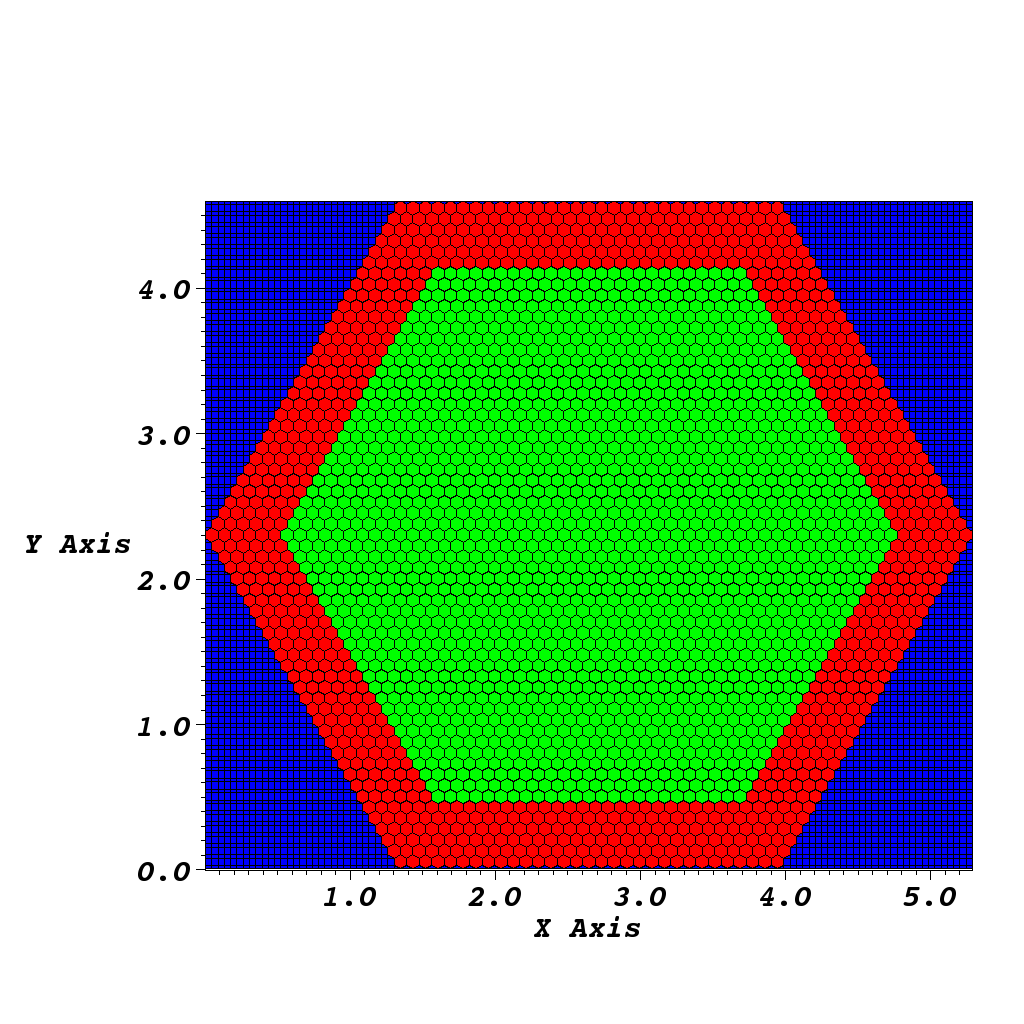
\includegraphics[width=0.4\textwidth]{./Dsa/source_crop}
\caption{Zones of the domain.}
\end{figure}
The properties of the different zones are:
\begin{description}
\item[Green zone:] $\Sigma_t =1$cm$^{-1}$, $\Sigma_s = 0.9$cm$^{-1}$, source$ =
1$cm$^{-3}$s$^{-1}$
\item[Red zone:] $\Sigma_t = 1.5$cm$^{-1}$, $\Sigma_s = 1.44$cm$^{-1}$, no source
\item[Blue zone:] $\Sigma_t = 1$cm$^{-1}$, $\Sigma_s = 0.3$cm$^{-1}$, no source
\end{description}
The scalar flux for this problem is:
\begin{figure}[H]
\centering
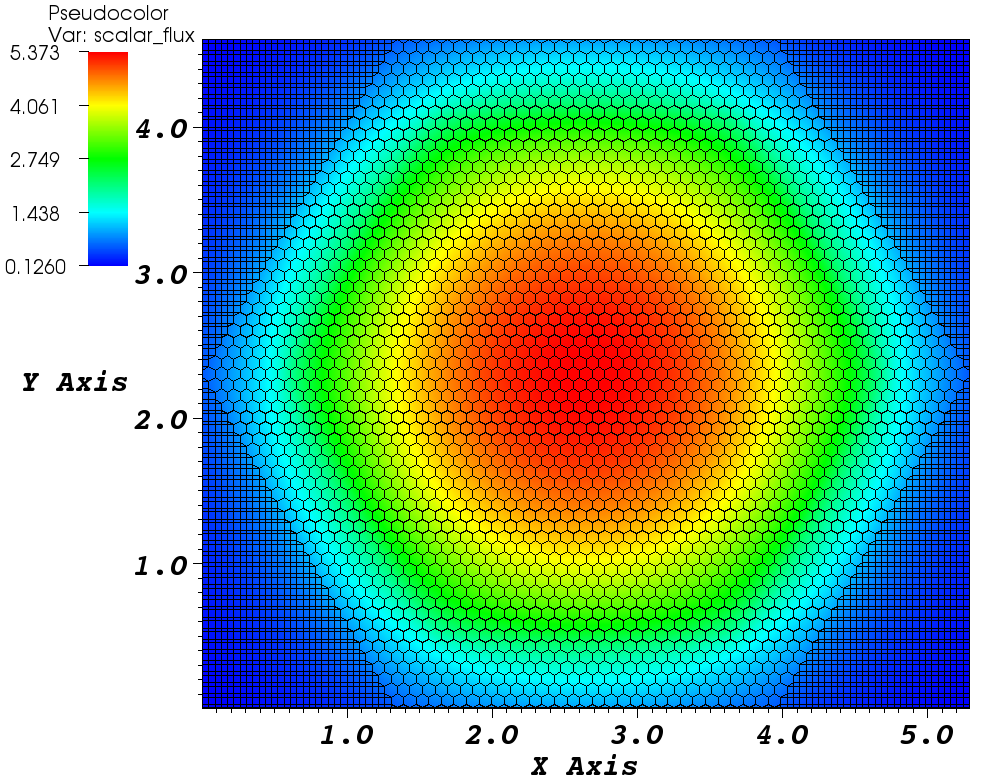
\includegraphics[width=0.6\textwidth]{./Dsa/heterog_hex_crop}
\caption{Scalar flux on a mesh composed of hexagonal cells.}
\end{figure}
The different solvers are compared in the next Table:
\begin{table}[H]
\begin{center}
\caption{Comparison of different preconditioners for a heterogeneous medium.}
\begin{tabular}{|c|c|c|c|c|c|c|}
\hline
 & No-DSA & CG & PCG-SGS & PCG-MLU & PCG-MLM & AGMG\\
\hline
  SI iter & 111     & 19      & 19        & 19      & 19      & 19 \\
 Prec (s) & NA      & NA      & 0.0159521 & 0.49212 & 1.31818 & 0.108 \\
  MIP (s) & NA      & 51.7628 & 82.5123   & 30.987  & 29.7762 & 2.64274 \\
   G iter & NA      & 10216   & 4481      & 423     & 402     & 260 \\
Total (s) & 379.175 & 121.798 & 147.094   & 94.7139 & 94.8013 & 65.5546 \\
\hline
\end{tabular}
\end{center}
\end{table}
We can see that the comments that were done for the homogeneous tests are
still valid. MIP is effective even with heterogeneous medium and AGMG is
still the fastest solver.

\section{Conclusions} \label{sec_conc}
We have adapted the MIP-DSA to PieceWise Linear Discontinuous finite elements
and proposed a simple way to compute the penalty coefficient which allows the
use of MIP on arbitrary polygonal meshes. The advantage being the potential reduction 
of the numbers of unknowns and the possibility to use adaptive mesh refinement 
without having hanging nodes. We have performed two Fourier analysis of the
new MIP-DSA on rectangular cell and shown that MIP is always stable when the
scattering is isotropic. On three different examples, we tested MIP on highly
unstructured meshed composed of different types of cells. We noticed that the
efficiency of MIP does not seem to be degraded on these meshes. We have also
compared different preconditioners for CG to solve MIP. Algebraic multigrid
methods were found to be the best preconditioner, AGMG being up to 20 times
faster than CG without preconditioning which itself was faster than CG
preconditioned by SSOR.




\chapter{\uppercase{Janus}}
\label{janus_chapter}
\section{Introduction}
In this Chapter, we detail the implementation of the transport code developed
in this research, Janus. Janus is a two-dimensional one-group $S_n$ transport
solver. It uses arbitrary polygonal meshes and implements an angular multigrid
preconditioner for highly anisotropic medium. The ASCII output file generated
by Janus can be converted to a silo file \cite{silo}, using an other C++ code,
Apollo. This output file can be read by VisIt \cite{visit}. A python code, 
Diana, can be used to generate the mesh or to convert a mesh generated by Triangle
\cite{triangle} into a mesh readable by Janus. Another python code, Mercury,
can be used to generate input file for Janus. Mercury can help writing an
input by checking that all the data required by Janus are present and that
they are written in the right order. 

Janus is documented using Doxygen \cite{doxygen}. It is built upon Trilinos
10.4 \cite{trilinos} and GSL (GNU Scientific Library) \cite{gsl} and uses
Autoconf, Automake, and Autotest \cite{autoconf,automake}. Git \cite{git} 
is used for revision control. 

Janus, Diana, and Mercury can be cloned at 
\emph{\hbox{git://gitorious.org/transport/janus.git}} 

Apollo can be cloned at \emph{\hbox{git://gitorious.org/transport/plot.git}}


\section{Implementation}
Janus is composed of the following classes:
\begin{description}
  \item[PARAMETERS:] In this class, the different parameters such as, the 
    type of solver for transport equation (SI or a Krylov method), the type 
    of solver for MIP, the convergence tolerance, the boundary conditions, 
    the intensity of the sources, the cross sections, etc, are read from an
    input file and stored. If Fokker-Planck cross sections are used, they 
    are computed here. The different cross sections for the angular
    multigrid are computed by this class and the extended transport correction 
    is applied.
  \item[TRIANGULATION:] In this class, the geometry, the material ids, and the
    source ids are read. Two different input files can be read. When the mesh
    uses rectangular cells, the abscissae then the ordinates have to be given 
    in increasing value. After that, the materials ids and the source ids are
    read. For instance, if the domain, $1cm \times 1cm$, is decomposed 
    in four identical cells, the input file looks like:
    \begin{verbatim}
    rectangle
    2 2      // (number of x-divisions, number of y-divisions)
    0. 0.5 1.0
    0. 0.5 1.0
    0 0 0 0  // (material ids)
    0 0 0 0  // (source ids)
    \end{verbatim}
    The other acceptable type of input file is used for polygonal cells. In 
    that case, the number of edges of a cell is given first, followed by the 
    coordinates of each vertex, the material ids and finally the source ids.
    The vertices must be ordered in an anti-clockwise order but there is no need
    to order the cell or for two successive cells to be adjacent in the mesh. 
    For instance, a possible input file would be:
    \begin{verbatim}
    polygon
    4   // (number of cells)
    3 1. 0. 1. 1. 0.5 0.5 0 0
    5 0. 0. 0.5 0. 0.5 0.5 0.5 1. 0. 1. 0 0
    3 0.5 0. 1. 0. 0.5 0.5 0 0
    3 0.5 0.5 1. 1. 0.5 1. 0 0
    \end{verbatim}
    This class assumes that the domain is rectangular. After reading the
    geometry, the EDGE objects are created. Before an edge is created, it must
    be checked that the edge does not already exist. To do so, the coordinates
    of the two vertices of the candidate edge are compared with the
    coordinates of the vertices of a subset of the existing edge. This subset
    corresponds to the smallest subset of edges having an abscissa,
    respectively an ordinate, of one of their vertices equals to an abscissa,
    respectively an ordinate, of one of the vertices of the candidate edge.
  \item[EDGE:] This class contains the coordinates of the vertices associated
    to the edge, the global and local ids of the edge, the ids of the cells 
    associated to the edge, the type of cell (interior or on the boundary and 
    the type of boundary: vacuum, isotropic or most normal direction of the
    quadrature), the two normals associated to the two cells, the 
    length of the edge, etc.
  \item[FINITE\_ELEMENT:] This class is the base class for BLD and PWLD.
    It contains all the matrices needed for the discretization of the transport
    equation and of MIP.
  \item[BLD:] This class derives from FINITE\_ELEMENT and builds the bilinear
    finite elements.
  \item[PWLD:] This class derives from FINITE\_ELEMENT and builds the
    piecewise linear finite elements.
  \item[QUADRATURE:] This class is the base class for GLC and LS. QUADRATURE
    builds the discrete-to-moment and moment-to-discrete matrices and
    stores the different directions used by the quadrature. The
    directions on the first octant are computed in GLC and LS. Then, they are
    deployed over the other octants. After that, the spherical harmonics
    are computed and evaluated at the given directions. When a Galerkin
    quadrature is used, selection rules are employed and the discrete-to-moment
    matrix is computed by inverting the moment-to-discrete matrix. Otherwise,
    the discrete-to-moment matrix is obtained by transposing the moment-to-discrete
    matrix and by multiplying it by the weights of the quadrature.
  \item[GLC:] This class derives from QUADRATURE and computes the weights and
    the directions used by the Gauss-Legendre-Chebyshev quadrature.
  \item[LS:] This class derives from QUADRATURE and computes the weights and
    the directions used by the Level-Symmetric quadrature.
  \item[CELL:] This class stores the id of cell, a vector of pointers to the
    edges of cell, the intensity of the source in the cell, the material
    properties ($\Sigma_s$, $\Sigma_t$, and the diffusion coefficient), 
    the FINITE\_ELEMENT associated to the cell, etc. The orthogonal lengths are
    calculated by this class.
  \item[DOF\_HANDLER:] This class builds the \emph{mesh} by creating all the 
    CELL objects and the  FINITE\_ELEMENT objects associated to them. It is 
    the DOF\_HANDLER object that computes the sweep
    ordering for all the directions. First, the edges on the boundary with a
    known incoming flux are put in a list \emph{incoming\_edges}. The sweep
    ordering will continue as long as this list is not empty. The first edge 
    in the list is popped and the cell associated is found. When the edge is 
    interior, the cell which has not been accepted in the sweep order is popped.
    Then, we loop over the edges of the cell to determine which ones are
    associated to an outgoing flux and which ones are associated to an
    incoming flux. The cell is accepted if all the
    edges which are not ``outgoing'' are in \emph{incoming\_edges}. If the cell is
    rejected, the edge is pushed back at the end of the list. If the cell is
    accepted, the edges of the cell which are incoming are removed from
    \emph{incoming\_edges}. The others edges are pushed back are the end of the
    list except if they are on the boundary of the domain. Because of the 
    symmetry of the quadratures used, the sweep orders have to be computed 
    for only half the directions. The sweep orders for the other directions 
    are just the opposite of the ones calculated.
  \item[TRANSPORT\_OPERATOR:] This class is the one where the calculation is
    made. It derives from the Epetra\_Operator of Trilinos.
    TRANSPORT\_OPERATOR handles the angular multigrid by calling itself
    recursively and restricting and projecting the flux moments on the
    different ``angular'' grids. It is also in this class that the scattering 
    source is computed and the sweeps are  performed. 
  \item[MIP:] This class builds and solves MIP. The first time that
    \emph{Solve()} is called, the left hand-side is built and stored using a 
    compressed row storage format (CRS). Then, the problem is
    solved by CG, PCG-SSOR, PCG-MLU, PCG-MLM, or AGMG. If AGMG is employed, 
    there is an extra step to convert the right hand-side to Fortran data type 
    and the  result to an Epetra\_MultiVector.
  \item[TRANSPORT\_SOLVER:] This class builds the PARAMETERS object, the
    TRIANGULATION object, the QUADRATURE object(s), the DOF\_HANDLER object,
    and the initial TRANSPORT\_OPERATOR object. SI and the Krylov solvers are
    called in \emph{Solve()}. The final result and the mesh are written in a file
    by this class.
  \item[EXCEPTION:] This class handles the exceptions that can be thrown.
\end{description}

\section{Verifications}
The verification of the code was done through unit testing, comparisons of
results with existing codes, and using known solutions of problems. Next, we
show two of the tests that were done to check the code.
\subsection{Infinite medium}
When the domain is infinite and the medium is homogeneous. The isotropic
transport equation reduces to:
\begin{equation}
  \phi = \frac{Q}{\Sigma_a}.
  \label{ez_pz}
\end{equation}
To approximate the infinite medium, we choose a very large total cross section
such that the mean free path of the particles is very small compared to the
size of the domain. In the following test, the domain is $1000cm \times
1000cm$, $Q = 2 n/(cm^3s)$, $\Sigma_t = 10 cm^{-1}$ and $\Sigma_s = 9
cm^{-1}$. We use vacuum boundary conditions and a $S_{8}$ GLC quadrature.
We show two tests: one which uses an uniform mesh of 100 by 100 cells and BLD
finite elements and the other which uses an unstructured mesh of 9972
quadrilaterals and PWLD finite elements. Given \cref{ez_pz}, the scalar flux
should be equal to two. In Figures \ref{quad_diff} and \ref{poly_diff}, the 
scalar flux less than or equal to 1.999 is in blue and the scalar flux greater
than or equal to 2.001 is in red:
\begin{figure}[H]
  \centering
  \subfloat[Rectangular cells]{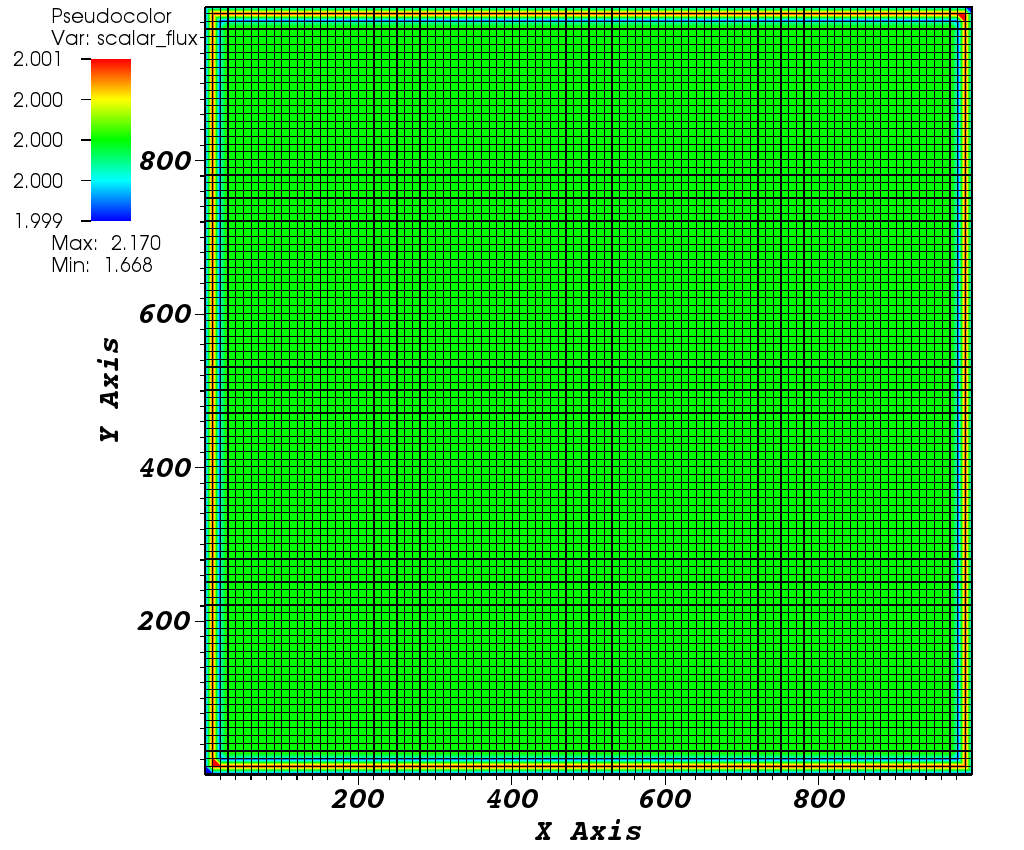
\includegraphics[width=0.63\textwidth]
  {./Janus/quad_diff}\label{quad_diff}}\\
  \subfloat[Quadrilateral cells]{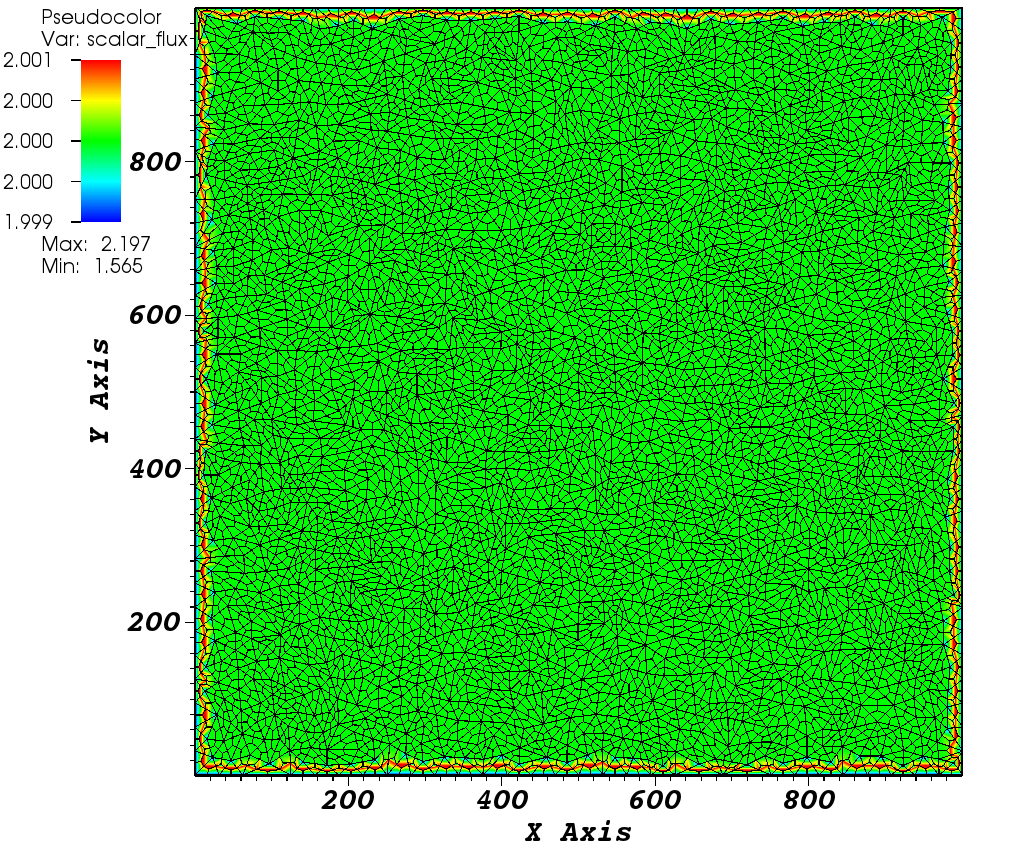
\includegraphics[width=0.63\textwidth]
  {./Janus/poly_diff}\label{poly_diff}}
  \caption{Scalar flux}
\end{figure}
\subsection{Convergence order}
In this test, we check the convergence order of PWLD and BLD on a benchmark.
We plot the error on average scalar fluxes as a function of the number of 
degrees of freedom. Since for two-dimensional geometries, the number of
degrees of freedom is
proportional to the square of the typical element size, the slopes of the 
graphs should equal one (PWLD and BLD are both second order methods). The test
that we chose is the IAEA EIR-2 benchmark problem \cite{Khalil1985}. This 
benchmark consists of five regions:
\begin{figure}[H]
  \centering
  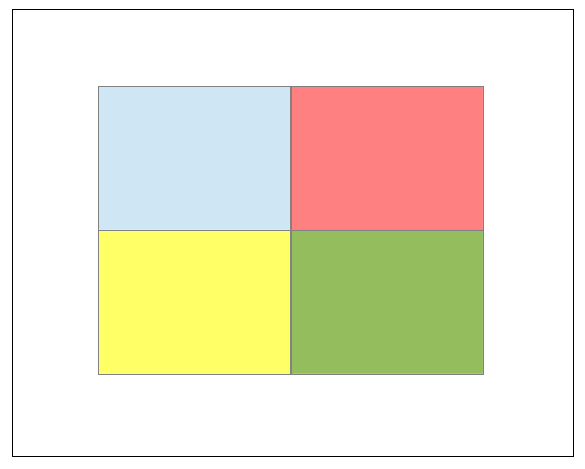
\includegraphics[width=0.4\textwidth]{./Janus/benchmark}
  \caption{Zones of the IAEA EIR-2 benchmark problem}
\end{figure}
The properties of the different zones are given in Table \ref{tabl_1}:
\begin{table}[H]
  \begin{center}
    \caption{Properties of the different zones of the benchmark}
    \begin{tabular}{|c|c|c|c|c|c|}
      \hline
    Zone & White & Blue & Salmon & Yellow & Green \\
      \hline
      Source $(n/(cm^3s))$ & 0    & 0    & 1    & 1    & 0 \\
    $\Sigma_t$ $(cm^{-1})$ & 0.9  & 0.65 & 0.7  & 0.6  & 0.48 \\
    $\Sigma_s$ $(cm^{-1})$ & 0.89 & 0.5  & 0.66 & 0.53 & 0.2 \\
             length ($cm$) & 96   & 30   & 30   & 30   & 30 \\
             height ($cm$) & 86   & 25   & 25   & 25   & 25 \\
      \hline
    \end{tabular}
    \label{tabl_1}
  \end{center}
\end{table}
The colored zones are in the middle of the white zone. In Figures \ref{glc_bld} 
and \ref{glc_pwld}, we show the convergence of the average scalar flux in the
different zones for $S_8$ Gauss-Legendre-Chebyshev quadrature when BLD and PWLD 
finite elements are used.
\begin{figure}[H]
  \centering
  \subfloat[BLD finite elements]{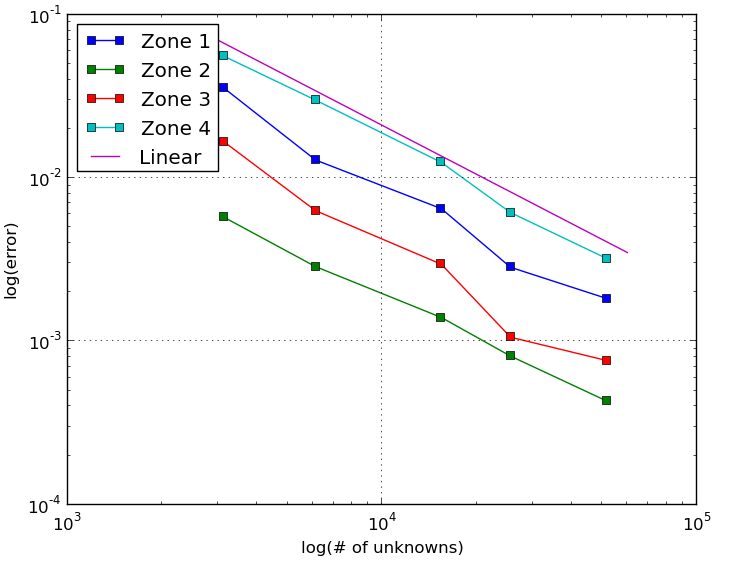
\includegraphics[width=0.5\textwidth]
  {./Janus/glc_conv_bld}\label{glc_bld}}
  \subfloat[PWLD finite elements]{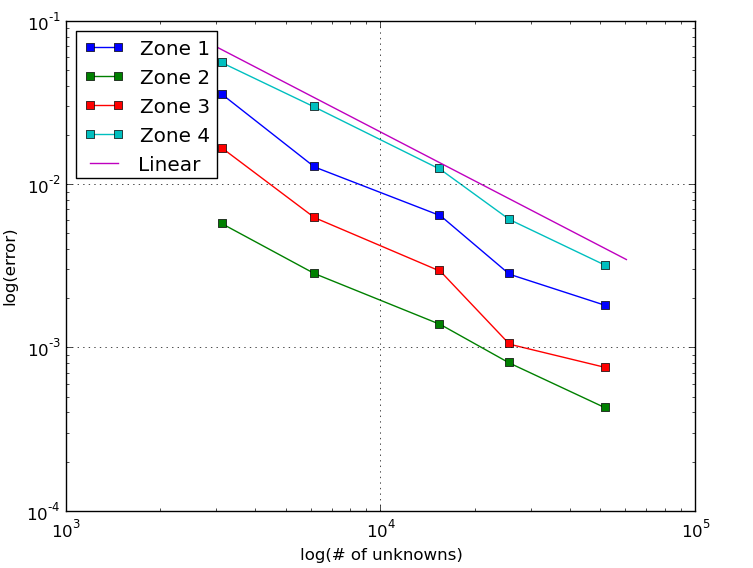
\includegraphics[width=0.5\textwidth]
  {./Janus/glc_conv_pwld}\label{glc_pwld}}
  \caption{Convergence of BLD and PWLD}
\end{figure}
We can see that the curves in all the zones have the right slope, i.e.,
the right order of convergence.



\section{Conclusions} \label{sec_conc}
We have adapted the MIP-DSA to PieceWise Linear Discontinuous finite elements
and proposed a simple way to compute the penalty coefficient which allows the
use of MIP on arbitrary polygonal meshes. The advantage being the potential reduction 
of the numbers of unknowns and the possibility to use adaptive mesh refinement 
without having hanging nodes. We have performed two Fourier analysis of the
new MIP-DSA on rectangular cell and shown that MIP is always stable when the
scattering is isotropic. On three different examples, we tested MIP on highly
unstructured meshed composed of different types of cells. We noticed that the
efficiency of MIP does not seem to be degraded on these meshes. We have also
compared different preconditioners for CG to solve MIP. Algebraic multigrid
methods were found to be the best preconditioner, AGMG being up to 20 times
faster than CG without preconditioning which itself was faster than CG
preconditioned by SSOR.



% bibliography
\addcontentsline{toc}{part}{REFERENCES}
\renewcommand{\bibname}{{\normalsize\rm REFERENCES}}
\bibliographystyle{plain}
\bibliography{biblio}


% appendix
\titleformat{\chapter}{\centering\normalsize}{APPENDIX \thechapter.}{1em}{}
\begin{appendices}
\renewcommand{\appendixname}{\uppercase{Appendix}}
%\renewcommand{\appendixtitle}{\uppercase{Appendix}}

\chapter[ ]{\uppercase{ML options}}

Some of the available coarsening schemes in ML \cite{ml_guide}:
\begin{description}
  \item[Uncoupled:] Attempt to construct aggregates of optimal size ($3^d$
    nodes in $d$ dimensions). Each process works independently and aggregates
    cannot span processes.
  \item[MIS:] Uses maximal independent set techniques to define aggregates.
    Aggregates can span processes. May provide better quality aggregates than
    {\bf Uncoupled}, but computationally more expensive because it requires
    matrix-matrix product.
\end{description}
Some of the smoothers:
\begin{description}
  \item[Jacobi]
  \item[Symmetric Gauss-Seidel]
\end{description}
Some of the coarse solvers:
\begin{description}
  \item[Jacobi]
  \item[Symmetric Gauss-Seidel]
  \item[Amesos-KLU:] Use {\bf KLU} through {\bf Amesos}. Coarse grid problem
    is shipped to processor 0, solved, and solution is broadcast.
  \item[Amesos-UMFPACK:] Use {\bf UMFPACK} through {\bf Amesos}. Coarse grid
    problem is shipped to processor 0, solved, and solution is broadcast.
  \item[Amesos-MUMPS:] Use double precision version of {\bf MUMPS} through
    {\bf Amesos}.
\end{description}
The MultiLevelPreconditioner class provide default values for five different
preconditioner types:
\begin{itemize}
  \item Classical smoothed aggregation for symmetric and positive definite or
    nearly symmetric and definite systems (used here)
  \item Classical smoothed aggregation-based two-level domain decomposition.
  \item Three-level algebraic domain decomposition.
  \item Eddy current formulation of Maxwell's equation.
  \item Energy-based minimizing smoothed aggregation suitable for highly
    convective nonsymmetric fluid flow problems.
\end{itemize}
The options used in this work are:
\begin{description}
  \item[option name:] SA
  \item[max levels:] 10
  \item[prec type:] $V-$cycle
  \item[aggregation type:] uncoupled-MIS
  \item[aggregation damping factor:] 4/3
  \item[eigen-analysis type:] cg
  \item[eigen-analysis iterations:] 10
  \item[smoother sweeps:] 2
  \item[smoother damping factor:] 1.0
  \item[smoother pre or post:] both
  \item[smoother type:] symmetric Gauss-Seidel
  \item[coarse type:] Amesos-KLU
  \item[coarse max size:] 128
\end{description}


\end{appendices}
\pagebreak{}


\end{document}

